%% This is file `example.tex',

%% generated with the docstrip utility.
%%
%% The original source files were:
%%
%% coppe.dtx  (with options: `example')
%% 
%% This is a sample monograph which illustrates the use of `coppe' document
%% class and `coppe-unsrt' BibTeX style.
%% 
%% \CheckSum{1620}
%% \CharacterTable
%%  {Upper-case    \A\B\C\D\E\F\G\H\I\J\K\L\M\N\O\P\Q\R\S\T\U\V\W\X\Y\Z
%%   Lower-case    \a\b\c\d\e\f\g\h\i\j\k\l\m\n\o\p\q\r\s\t\u\v\w\x\y\z
%%   Digits        \0\1\2\3\4\5\6\7\8\9
%%   Exclamation   \!     Double quote  \"     Hash (number) \#
%%   Dollar        \$     Percent       \%     Ampersand     \&
%%   Acute accent  \'     Left paren    \(     Right paren   \)
%%   Asterisk      \*     Plus          \+     Comma         \,
%%   Minus         \-     Point         \.     Solidus       \/
%%   Colon         \:     Semicolon     \;     Less than     \<
%%   Equals        \=     Greater than  \>     Question mark \?
%%   Commercial at \@     Left bracket  \[     Backslash     \\
%%   Right bracket \]     Circumflex    \^     Underscore    \_
%%   Grave accent  \`     Left brace    \{     Vertical bar  \|
%%   Right brace   \}     Tilde         \~}
%%
\documentclass[dsc,english]{coppe}
\usepackage{natbib}
\usepackage{amsmath,amssymb}
\usepackage{hyperref}
\usepackage{amssymb}
\usepackage{tikz}
\usepackage{multirow}
\usepackage{amsmath}
\usepackage{booktabs} 
\usepackage{subcaption}
\usepackage{amsthm}
\usepackage{url}
\usepackage{lineno}
\usepackage{enumerate}

\newtheorem{definition}{Definition}
\newtheorem{theorem}{Theorem}
\newtheorem{hypothesis}{Hypothesis}
\DeclareMathOperator*{\argmin}{arg\,min}
\DeclareMathOperator{\FTL}{FTL}



\linenumbers % Enable line numbering
\modulolinenumbers[5] % Set line numbering interval


\makelosymbols
\makeloabbreviations

\begin{document}
  \title{Função de custo e penalização robustas para aprendizado de máquina justo}
  \foreigntitle{Robust loss and penalty to fair machine learning}
  \author{Ygor}{de Mello Canalli}
  \advisor{Prof.}{Geraldo}{Zimbrão da Silva}{D.Sc.}
  \advisor{Prof.}{Filipe}{Braida do Carmo}{D.Sc.}

  \examiner{Prof.}{Geraldo Zimbrão da Silva}{D.Sc.}
  \examiner{Prof.}{Filipe Braida do Carmo}{D.Sc.}
  \examiner{Prof.}{Geraldo Bonorino Xexéo}{D.Sc.}
  \examiner{Prof.}{Daniel Sadoc Menasché}{Ph.D}
  \examiner{Prof.}{Carlos Eduardo Ribeiro de Mello}{Ph.D.}
  \department{PESC}
  \date{08}{2024}

  \keyword{Fair machine learning}
  \keyword{Label noise robustness}
  \keyword{Multi-objective optimization}
  \keyword{Redlining effect}

  \maketitle

  \frontmatter
  \dedication{A algu\'em cujo valor \'e digno desta dedicat\'oria.}

  \chapter*{Agradecimentos}

  Gostaria de agradecer a todos.

  \begin{abstract}

A ampla adoção de aprendizado de máquina em decisões de impacto social expandiu sistematicamente a aplicação de padrões discriminatórios já existentes. Assim, técnicas de aprendizado de máquina justas tornaram-se uma fronteira para pesquisadores e profissionais de IA. Abordar a equidade é complexo, não se pode depender apenas dos dados usados para treinar modelos ou das métricas que os avaliam, pois esses dados frequentemente são a principal fonte de viés, similar a dados ruidosos. Exploramos a convergência entre equidade e ruído no aprendizado de máquina, destacando semelhanças e diferenças. Apresentamos “Fair Transition Loss”, um novo método para classificação justa inspirado em técnicas de robustez contra ruído de rótulo. Funções de custo convencionais ignoram a distribuição dos dados sensíveis e seu impacto nas previsões. Nossa abordagem utiliza matrizes de transição para ajustar as previsões utilizando estes dados ignorados. Nossa avaliação empírica usando o teste de significância de ordem quase-estocástica indica que esse método supera muitas abordagens clássicas e de ponta na maioria dos conjuntos de dados de referência e objetivos de otimização. Além disso, a abordagem proposta se mostrou a única a manter resultados competitivos em todos os cenários.

Além disso, apresentamos uma abordagem de regularização inovadora denominada “Redlining Penalty Regularization”, que penaliza proporcionalmente a dependência do modelo de preditores indiretos dos atributos sensíveis de acordo com suas correlações. Nossos resultados experimentais demonstram que a técnica proposta melhora os resultados tanto em redes neurais convencionais quanto naquelas treinadas usando o “Fair Transition Loss” em uma variedade de conjuntos de dados e objetivos de otimização para classificação justa.

  \end{abstract}

  \begin{foreignabstract}

The Machine learning widespread adoption has inadvertently led to the amplification of societal biases and discrimination, with many consequential decisions now influenced by data-driven systems. In this scenario, fair machine learning techniques has become a frontier for AI researchers and practitioners. Addressing fairness is intricate; one cannot solely rely on the data used to train models or the metrics that assess them, as this data is often the primary source of bias — akin to noisy data. This work delves into the convergence of these two research domains, highlighting the similarities and differences between fairness and noise in machine learning. We introduce the Fair Transition Loss, a novel method for fair classification inspired by label noise robustness techniques. Traditional loss functions tend to ignore distributions of sensitive features and their impact on outcomes. Our approach uses transition matrices to adjust predicted label probabilities based on this ignored data. The empirical evaluation using Almost Stochastic Order significance test indicates that this method outperforms many classical and state-of-art approaches in most of benchmarked datasets and optimization objectives to fair classification. Additionally, the proposed approach remains as the only to keep competitive results on all compared scenarios.

Also, we present the Redlining Penalty Regularization, a novel regularization approach that proportionately penalizes model’s dependency on sensitive feature proxies according their correlations. Our experimental results demonstrates that this proposed technique improves both results on standard neural networks and those trained using Fair Transition Loss on a variety of datasets and optimization objectives to fair classification.

  \end{foreignabstract}

  \tableofcontents
  \listoffigures
  \listoftables
  \printlosymbols
  \printloabbreviations

  \mainmatter
  
  \chapter{Introduction}

The issue of fairness in machine learning has recently risen to prominence due to its implications in real-world decision-making systems~\citep{Mehrabi2019,Hutchinson2019}. Addressing biases and discrimination is a relevant frontier in decision-making systems, as equitable outcomes across various demographic groups is both an ethical imperative and often a legal requirement. Though fairness is a multifaceted concept, it has been deeply examined within the context of machine learning. The literature presents a variety of fairness definitions, drawing concepts from political philosophy and computational techniques~\citep{caton2023, Hutchinson2019}. Choosing an equitable machine learning model requires the selection of a fitting definition of fairness, tailored to the specific problem at hand. Many such definitions can be precisely articulated, allowing models to be evaluated based on their predictions.

One inherent challenge in fair machine learning is the balance between fairness and accuracy. Efforts to mitigate unfairness often compromise the model's predictive performance, a trade-off that has been well documented~\citep{Mehrabi2019, caton2023}. Predictors that are less biased against marginalized groups may deviate from the true class, resulting in sub-optimal performance. Also, introducing fairness considerations adds constraints to the model, further complicating the optimization process~\citep{Zafar2017b}. 

In light of these challenges, we introduce the Fair Transition Loss, a novel approach to fair classification. This method estimates the influence of historical and societal biases on outcome probabilities for distinct groups within dataset. For instance, individuals from marginalized groups might have lower chances of favorable outcomes compared to their counterparts from privileged groups. Such disparate probabilities can be represented by transition matrices. Drawing inspiration from label noise robustness, we incorporate these transition matrices information into the loss function to promote fairness. The proposed method has some hyperarameters, chosen by a Multi-Objective Optimization approach combining both fairness and model performance with a linear smooth objective. This objective is defined in such a way that it is possible to use this approach to optimize a variety of fairness and performance metrics.

The primary contribution of this study is the conceptualization of the Fair Transition Loss, a novel loss function influenced by label noise methodologies. In benchmark tests across common fair classification tasks, our empirical results demonstrate that this method consistently outperforms many leading in-processing fair classification techniques in a variety of scenarios. The novelty of this work lies in applying label noise techniques directly within the model to mitigate unfairness. As far as we know, this is the first time that label noise techniques are directly used to address fairness in machine learning.

%The remainder of this paper is structured as follows: Section~\ref{sec:related} delineates related works encompassing fairness definitions, metrics and methods, multi-objective optimization in fair machine learning, and classifications in the presence of label noise. We also spotlight studies bridging fairness and label noise. In Section~\ref{sec:proposal}, we describe the Fair Transition Loss and its underlying principles. Section~\ref{sec:experimental} details our experimental methodology and Section~\ref{sec:results} discuss results for common fair classification tasks. In Section~\ref{sec:conclusions} we present conclusions drawn from our study and insights to research directions.


\section{Contextualization}

\section{Objectives}

\section{Contributions}

\section{Results summary}

\section{Thesis structure}

  
\chapter{Fair Machine Learning Review}

The field of Machine Learning (ML) has experienced significant growth and is increasingly applied in various societal domains such as healthcare, finance, and criminal justice. This growth raises important ethical and operational concerns, particularly regarding the principles of Fairness, Accountability, and Transparency (FAT) \citep{Memarian2023}. As ML algorithms increasingly influence a wide array of societal domains, including criminal justice, healthcare, finance, and employment, the requirement to ensure these systems are designed and implemented responsibly has become paramount. This section aims to delineate the significance, scope, and prevailing challenges associated with integrating FAT principles into ML, providing a foundation for the subsequent discussion.

Fairness in ML concerns the equitable and just treatment of all individuals, particularly those from historically marginalized or disadvantaged groups \citep{Mehrabi2019, caton2023}. It seeks to ensure that ML algorithms do not perpetuate existing biases or create new forms of discrimination. However, the multifaceted nature of fairness, encompassing various definitions and metrics, poses substantial challenges in operationalizing it within algorithmic frameworks. Further in this section we will explore these complexities, examining different conceptions of fairness and the inherent trade-offs they entail.

Accountability in ML pertains to the obligation of designers, developers, and deployers of ML systems to be answerable for the outcomes of these systems \citep{Hutchinson2021}. It involves establishing mechanisms that allow for the tracing of decisions back to the entities responsible for the deployment of the ML algorithms. Accountability also encompasses the adherence to ethical standards, legal requirements, and societal norms. This discussion frequently involves mechanisms and practices that can promote accountability in ML, like auditing, documentation, and regulatory compliance.

Transparency, the third pillar, refers to the clarity and openness with which ML systems operate \citep{Burkart2021}. It involves the ability of stakeholders, including end-users, regulators, and the broader public, to understand how ML systems make decisions. Transparency is mandatory property of any automated decision making system to achieve trustworthyness, facilitating informed consent, and enabling the scrutiny necessary to identify and rectify biases. However, achieving transparency, particularly with complex models, presents its own set of technical and ethical challenges. This research topic includes isses as the trade-off between explainability and model performance, and discussing emerging approaches to tackle interpretability without sacrificing effectiveness.

The triad of Fairness, Accountability, and Transparency (FAT) alongwith data privacy forms the cornerstone of Trustworty Artificial Intelligence (TwAI). These principles are pivotal in ensuring that AI systems are developed and deployed in a manner that respects human rights, promotes social well-being, and maintains public trust. While accountability ensures that entities behind AI systems can be held responsible for their outcomes, transparency allows stakeholders to produce and maintain environments where AI systems can be scrutinized, understood, and corrected, thereby aligning their functionality with societal norms and values.

In this context of Trustworty AI the European Union's High-Level Expert Group on Artificial Intelligence has outlined seven key principles that aim to ensure that AI systems are designed and used in a way that is ethically sound and trustworthy~\citep{TwAI_Europe}. These principles are fundamental for developing and maintaing decision making systems that are beneficial and avoid unintended harm. The seven principles are as follows:

\begin{description}
    \item[Human agency and oversight] AI systems should empower human beings, allowing them to make informed decisions and fostering their fundamental rights. At the same time, proper oversight mechanisms need to be ensured, which can be achieved through human-in-the-loop, human-on-the-loop, and human-in-command approaches
    \item[Technical Robustness and safety] AI systems need to be resilient and secure. They need to be safe, ensuring a fall back plan in case something goes wrong, as well as being accurate, reliable and rep roducible. That is the only way to ensure that also unintentional harm can be minimized and prevented.
    \item[Privacy and data governance] besides ensuring full respect for privacy and data protection, adequate data governance mechanisms must also be ensured, taking into account the quality and integrity of the data, and ensuring legitimised access to data.
    \item[Transparency] the data, system and AI business models should be transparent. Traceability mechanisms can help achieving this. Moreover, AI systems and their decisions should be explained in a manner adapted to the stakeholder concerned. Humans need to be aware that they are interacting with an AI system, and must be informed of the system’s capabilities and limitations.
    \item[Diversity, non-discrimination and fairness] Unfair bias must be avoided, as it could have multiple negative implications, from the marginalization of vulnerable groups, to the exacerbation of prejudice and discrimination. Fostering diversity, AI systems should be accessible to all, regardless of any disability, and involve relevant stakeholders throughout their entire life circle.
    \item[Societal and environmental well-being] AI systems should benefit all human beings, including future generations. It must hence be ensured that they are sustainable and environmentally friendly. Moreover, they should take into account the environment, including other living beings, and their social and societal impact should be carefully considered. 
    \item[Accountability] Mechanisms should be put in place to ensure responsibility and accountability for AI systems and their outcomes. Auditability, which enables the assessment of algorithms, data and design processes plays a key role therein, especially in critical applications. Moreover, adequate an accessible redress should be ensured.
\end{description}


Although there are many aspects to consider to an ethical automated decision system with social impacts, the present text will concentrate predominantly on the aspect of fairness and negative social bias. Fairness is not only desirable for the development of just and equitable technological solutions but an obligation for maintaining the trustworthyness and acceptability of AI systems in diverse societal contexts.

\section{Sources and types of algorithmic unfairness}

The comprehensive survey conducted by \citet{Mehrabi2019} elucidates the multitude of biases that can pervade artificial intelligence applications, potentially leading to unfair outcomes. This analysis categorizes the various sources of bias, illustrating the multifaceted ways in which such biases can infiltrate different stages of machine learning processes, ranging from the initial data collection phase to the final algorithmic processing. The following exposition provides a short delineation of these sources of bias. To a rich discussion on this topic - including references, examples and real cases where each source of bias can emerge - we recommend the reading of the original work. The discussion here is with the purpose of proper describing the complexity and multifaceted nature of unfairness in machine learning models.


\begin{description}
    \item[Historical Bias] This is the existing societal bias that reflects past and present inequalities and prejudices. Historical bias is present in the data even before any machine learning model has interacted with it, due to inherent social and cultural inequalities;
    
    \item[Representation Bias] Occurs when the data sample does not accurately represent the entire population or certain subgroups within it. This can lead to machine learning models that perform well on majority groups but poorly on underrepresented groups;

    \item[Measurement Bias] Arises when the data collected does not accurately measure the real-world constructs it purports to measure. This type of bias can occur due to flawed data collection instruments or processes that systematically misrepresent certain groups;
    
    \item[Evaluation Bias] This type of bias occurs during the performance evaluation of machine learning models, where the evaluation criteria or methods may favor one group over others, leading to biased assessments of model performance;

    \item[Aggregation Bias] Happens when incorrect assumptions are made about the homogeneity of groups within the data. Aggregation bias can lead to misleading conclusions if the differences within and between groups or subgroups are not properly accounted for;
    
    \item[Population Bias] Similar to representation bias, population bias occurs when statistics, demographics, representatives, and user characteristics are different in the user population represented in the dataset, leading to models that are not generalizable across different demographic groups;

    \item[Simpson’s Paradox] This is a statistical phenomenon where a trend appears in several different groups of data but disappears or reverses when these groups are combined;

    \item[Longitudinal Data Fallacy] Occurs when cross-sectional data is treated as longitudinal, leading to incorrect conclusions about data trends over time;

    \item[Sampling Bias] Introduced by non-random sampling procedures, where certain members of the intended population are less likely to be included in the sample than others, leading to skewed data that does not accurately represent the entire population;
    
    \item[Behavioral Bias] Arises from variations in user behavior that differ across different platforms or contexts, affecting the data's representation of real-world phenomena;

    \item[Content Production Bias] Results from differences in how content is generated by different groups, with structural, lexical, semantic, and syntactic differences, influencing the data available for machine learning models; 

    \item[Linking Bias] Occurs in networked data, where the connections between nodes can misrepresent the true attributes or behavior of the nodes;

    \item[Temporal Bias] Reflects changes in data characteristics over time, due changes in representation or behaviors, which may not be accounted for in static machine learning models;
    
    \item[Popularity Bias] Occurs when popular items are more likely to be recommended or rated highly, not necessarily because of their quality but simply because of their initial, higher visibility and these popularity metrics are subject of mapinupation;

    \item[Algorithmic Bias] Introduced by the algorithms themselves, when they add bias that was not present in the input data:

    \item[User Interaction Bias] Results from the way system design influences user behavior in biased ways. This source of bias can be influenced by other types or subtypes, such as Presentation and Ranking Biasese:
    \begin{description}
        \item[Presentation Bias] This bias occurs when the way information is presented influences the outcomes. In machine learning, this can manifest through the design of user interfaces or the manner in which data is displayed, affecting user decisions and interactions;

        \item[Ranking Bias] Arises when algorithms prioritize certain data points over others in ranked lists or search results, which can distort visibility and perpetuate certain preferences or discriminations;
    \end{description}
    
    \item[Social Bias] Social biases are the preconceived notions and stereotypes held by societies, where individual actions or contents are socially influenced. These biases often find their way into data through collective social behaviors and decisions, influencing the training data used for machine learning models;

    \item[Emergent Bias] Emerges during the operation of a system, particularly as a result of changes in population, cultural values, or societal knowledge in the data over time. This type of bias is dynamic and can occur even if the initial model was unbiased, due to changes in the underlying data or context;

    \item[Self-Selection Bias] Occurs when the individuals selected for a study or dataset have self-selected in some way, producing a sample that is not representative of the general population. This can skew results and make the data less generalizable;

    \item[Omitted Variable Bias] Happens when a model overlooks certain relevant variables that are correlated with both the independent and dependent variables. Omitting these variables can lead to incorrect inferences about correlations and effects;

    \item[Cause-Effect Bias] This bias is a misunderstanding in the determination of causation; it can occur when correlations are mistaken for causal relationships without proper justification through causal inference techniques;

    \item[Observer Bias] Introduced by the expectations or preconceptions of those collecting or processing data, which can influence the outcomes subconsciously.;
    
    \item[Funding Bias] Refers to the influence that the source of funding can have on the conduct of research or development of algorithms. This type of bias can lead to results that favor the interests of the funding source, consciously or unconsciously.
\end{description}

These biases can pervade various stages of machine learning, from data collection to model evaluation and deployment, highlighting the importance of understanding and mitigating bias to achieve fairness in AI systems. Furthermore, the presence of biases can lead to feedback loops that exacerbate these inequalities over time. When biased data influence the decisions made by an AI system, these decisions can then be used to generate more data, which, if used to retrain the model, may reinforce and even amplify the existing biases. This cycle can create a self-perpetuating loop, making initial biases more entrenched and difficult to correct. Addressing feedback loops is critical, as they can progressively deteriorate the fairness of the system, leading to increasingly skewed outcomes that are harder to rectify. Effective strategies to break these loops include rigorous monitoring of model decisions, regular updates to training datasets to ensure diversity and representativeness, and the implementation of mechanisms that can detect and correct for emerging biases

Having outlined the various sources of unfairness in machine learning, \citet{Mehrabi2019} also explores different types of discrimination that arise from these biases. Understanding these types of discrimination is pivotal as they elucidate how biases, whether direct, indirect, systemic, statistical, explainable, or unexplainable, can culminate in unfair outcomes. Each type of discrimination demonstrates a distinct pathway through which biases embedded in data or algorithms manifest in practices and decisions, thus potentially perpetuating unfairness in AI systems. This comprehensive analysis helps in identifying targeted strategies to mitigate these discriminatory effects and underscores the importance of developing automated decision systems that are both just and equitable.


\begin{description}
    \item[Direct Discrimination] occurs when outcomes are directly affected by sensitive attributes such as race, gender, or age. This type of discrimination happens explicitly and is frequently legally prohibited;
    
    \item[Indirect Discrimination] manifests when proxy attributes indirectly linked to sensitive attributes influence outcomes. For example, using zip codes in decision-making processes might inadvertently reflect racial biases because residential areas often correlate with racial demographics. This phenomena is also refered as redlining effect~\citep{Pedreschi2008};
    
    \item[Systemic Discrimination] involves policies or practices entrenched within an organization that perpetuate disadvantage for certain groups. This can stem from cultural biases embedded in the decision-making processes, often reflecting the preferences or biases of dominant groups;
    
    \item[Statistical Discrimination] refers to the use of general statistics on a group to make inferences about individuals from that group. This type of discrimination might arise when decision-makers use visible characteristics as proxies for other traits, leading to biased assessments;
    
    \item[Explainable Discrimination] is considered legally permissible if the differences in treatment or outcomes can be justified through legitimate and relevant attributes. For instance, differences in pay might be justified by the number of hours worked if this factor significantly influences earnings;
    
    \item[Unexplainable Discrimination] occurs when there is no justifiable reason for the disparate treatment or outcomes, making it illegal and ethically unacceptable. This type of discrimination requires interventions to ensure fairness and equality in decision-making processes.
\end{description}


\section{Fairness definitions and metrics}

This section aims to present some widely used definitions and metrics of fairness, as described by \cite{Verma2018} and summarized by \cite{Mehrabi2019} and \cite{caton2023}, providing a comprehensive overview for understanding and navigating the multifaceted dimensions of fairness in ML systems. Initially, we explore general considerations and intuitive aspects of fairness, setting the stage for a deeper understanding. This preliminary discussion lays the groundwork for understaining the nuanced nature of fairness notions within the context of ML. Following this, we will transition into formal definitions, where we will dissect and explain those metrics and concepts.

Even before this discussion, we emphasizes that no single fairness definition universally applies to all scenarios. The choice of a particular fairness definition and metric should be informed by ethical considerations grounded in the social context in which the model would be deployed~\citep{AlerTubella2022}. Selecting a fairness definition is not a purely technical matter, as it inevitably requires ethical and social considerations that should not be neglected~\citep{Alves2023}. Building fair machine learning models requires an interdisciplinary approach that engages all stakeholders, including specially those who are typically marginalized or underrepresented~\citep{Weinberg2022}.

A prevalent taxonomy within fairness literature differentiates fairness notions into group metrics and individual metrics. Group Fairness Metrics hinge on the principle that statistical measures — such as error rates, precision, and recall — ought to be equitably distributed across groups demarcated by sensitive attributes like race, gender, or age. The core premise of these metrics is that fairness is actualized when an algorithm exhibits consistent performance across diverse demographic segments.

Demographic Parity, for example, mandates uniformity in the rate of positive algorithmic outcomes across different groups, a standard that remains agnostic to the underlying base rates within each population segment. On the other hand, Equal Opportunity and Equalized Odds introduce a nuance to this conversation by tethering fairness to the true condition of outcomes. This refinement delineates a central differentiation within fairness metrics: some are predicated solely on predicted values (such as Demographic Parity), while others derive from the scope of the confusion matrix (Table~\ref{tab:confusion_matrix_definition}), also incorporating true value conditions (as seen in Equal Opportunity and Equalized Odds).

Individual Fairness Metrics, in contrast, introduce a more granular perspective to fairness, advocating that similar individuals should be treated similarly by the ML system. This approach diverges from group-level considerations, focusing instead on ensuring that the algorithm’s treatment is consistent for individuals who are alike in relevant aspects, barring their membership in different demographic categories. Individual fairness seeks to ensure a personalized sense of justice, where the algorithmic outcomes are solely reflective of pertinent attributes rather than biased by irrelevant factors associated with sensitive attributes. This concept champions the notion that fairness extends beyond group identities to recognize and respect the uniqueness of individual experiences and qualifications.

To establish the foundation for discussing fairness definitions and metrics, we commence with an examination of the confusion matrix, which is an essential instrument in machine learning to assessing the performance of classification algorithms. It constitutes a tabular visualization that delineates the correspondence between the true labels and the predicted outcomes generated by a model. For binary classification tasks, the confusion matrix is structured into four principal components: True Positives (TP), True Negatives (TN), False Positives (FP), and False Negatives (FN), as outlined in Table~\ref{tab:confusion_matrix_definition}. By providing a clear breakdown of these outcomes, the confusion matrix allows to calculate many key performance metrics such as accuracy, precision, recall, and the F1 score, providing comprehensive insights into the strengths and weaknesses of the classification model. Also, the computation of those metrics forms the basis for evaluating fairness across distinct demographic groups.

\begin{table}[h]
    \centering
    \caption{Confusion matrix of binary classification outcomes} \label{tab:confusion_matrix_definition}
    \begin{tabular}{cc|c|c|}
    \cline{3-4}
     & & \multicolumn{2}{c|}{\textbf{Predicted}} \\ \cline{3-4}
     & & Positive & Negative \\ \hline
    \multicolumn{1}{|c|}{\multirow{2}{*}{\textbf{Actual}}} & Positive & TP & FN \\ \cline{2-4}
    \multicolumn{1}{|c|}{} & Negative & FP & TN \\ \hline
    \end{tabular}
\end{table}


True Positives (TP) can be defined as the probability that the predictor correctly identifies a positive outcome when the true condition is positive. Using the conditional probability notation, it is expressed as $P(\hat{Y}=1|Y=1)$, indicating the probability that the predicted class $\hat{Y}$ is positive given that the actual class $Y$ is positive.

False Positives (FP) represent the probability that the predictor incorrectly identifies a positive outcome when the true class is negative. It is denoted as $P(\hat{Y}=1|Y=0)$, reflecting the probability that the predicted class $\hat{Y}$ is positive when the actual class $Y$ is negative.

False Negatives (FN) are defined as the probability that the predictor incorrectly identifies a negative outcome when the true class is positive. This is given by $P(\hat{Y}=0|Y=1)$, the probability that the predicted class $\hat{Y}$ is negative given that the actual class $Y$ is positive.

True Negatives (TN) correspond to the probability that the predictor correctly identifies a negative outcome when the true condition is negative. In conditional probability terms, it is $P(\hat{Y}=0|Y=0)$, indicating the probability that the predicted class $\hat{Y}$ is negative given that the actual class $Y$ is negative.

Now we proceed to more complex metrics that provides complementary insights into the performance of the classifier. These derived metrics, such as Positive Predictive Value (PPV), False Discovery Rate (FDR), and others, constitutes the basic elements of the confusion matrix to quantify the reliability of the predictions in various ways. By expressing these metrics in terms of conditional probabilities and confusion matrix components, we facilitate a comprehensive analysis of the classifier's behavior, providing resources to a proper evaluation of its fairness across different demographic groups.

\begin{definition}[Positive Predictive Value (PPV)]\label{def:ppv}
PPV, or precision, measures the proportion of correctly identified positive outcomes among all predicted positives. It is defined as the probability that the true condition is positive given the predicted condition is positive, $P(Y=1|\hat{Y}=1)$. In terms of the confusion matrix, PPV is calculated as $\frac{TP}{TP + FP}$, the ratio of true positives to the sum of true positives and false positives.
\end{definition}

\begin{definition}[False Discovery Rate (FDR)]\label{def:fdr}
FDR quantifies the rate of incorrect positive predictions. It is the probability that the true condition is negative when the predicted condition is positive, $P(Y=0|\hat{Y}=1)$. From the confusion matrix, FDR is computed as $\frac{FP}{TP + FP}$, indicating the proportion of false positives out of all predicted positives.
\end{definition}

\begin{definition}[Negative Predictive Value (NPV)]\label{def:npv}
NPV assesses the accuracy of negative predictions, representing the probability that the true condition is negative given the predicted condition is negative, $P(Y=0|\hat{Y}=0)$. NPV is derived from the confusion matrix as $\frac{TN}{TN + FN}$, the number of true negatives over the sum of true negatives and false negatives.
\end{definition}

\begin{definition}[False Omission Rate (FOR)]\label{def:for}
FOR indicates the likelihood of a false negative prediction. It corresponds to the probability that the true condition is positive when the predicted condition is negative, $P(Y=1|\hat{Y}=0)$. In the confusion matrix context, FOR is $\frac{FN}{TN + FN}$, representing the number of false negatives relative to all predicted negatives.
\end{definition}

\begin{definition}[True Positive Rate (TPR)]\label{def:tpr}
TPR, or recall, measures the proportion of actual positives that are correctly predicted. It is the probability that the predicted condition is positive given the true condition is positive, $P(\hat{Y}=1|Y=1)$. TPR is calculated as $\frac{TP}{TP + FN}$ in the confusion matrix, the ratio of true positives to the sum of true positives and false negatives.
\end{definition}

\begin{definition}[False Negative Rate (FNR)]\label{def:fnr}
FNR quantifies the rate of missed positive predictions. It is defined as the probability that the predicted condition is negative when the true condition is positive, $P(\hat{Y}=0|Y=1)$. FNR is derived from the confusion matrix as $\frac{FN}{TP + FN}$, indicating the proportion of false negatives out of the actual positives.
\end{definition}

\begin{definition}[True Negative Rate (TNR)]\label{def:tnr}
TNR, or specificity, indicates the accuracy of negative predictions, representing the probability that the predicted condition is negative given the true condition is negative, $P(\hat{Y}=0|Y=0)$. From the confusion matrix, TNR is computed as $\frac{TN}{TN + FP}$, the number of true negatives to the sum of true negatives and false positives.
\end{definition}

\begin{definition}[False Positive Rate (FPR)]\label{def:fpr}
FPR assesses the likelihood of incorrect negative predictions, calculated as the probability that the predicted condition is positive when the true condition is negative, $P(\hat{Y}=1|Y=0)$. FPR is given by $\frac{FP}{TN + FP}$ in the confusion matrix, the ratio of false positives to the sum of true negatives and false positives.
\end{definition}

As we transition from foundational metrics that directly stem from the confusion matrix, such as PPV and TPR, we now discuss standard performance metrics that assess classification models in a more comprehensive manner. These metrics, such as Accuracy and F1 are distinguished by their reliance on both classes to provide a more holistic evaluation.

\begin{definition}[Accuracy (Acc.)]\label{def:acc}
Probably the most widely usaed performence metric to classification problems, Accuracy is the proportion of true results, both true positives and true negatives, among the total number of cases examined. In terms of conditional probabilities, accuracy reflects the probability that the predicted condition is correct, both as a positive and negative outcome, given the actual conditions, and can be 
expressed as 
\begin{align*}
    P(\hat{Y}=Y) &= P(\hat{Y}=1|Y=1) \cdot P(Y=1) \\
    &+ P(\hat{Y}=0|Y=0) \cdot P(Y=0).
\end{align*}
Using the confusion matrix, accuracy is computed as $$\frac{TP + TN}{TP + TN + FP + FN}.$$
\end{definition}
    
\begin{definition}[Balanced Accuracy (Bal. Acc.)]\label{def:ba}
Balanced accuracy is an average of the true positive rate (TPR) and the true negative rate (TNR), which compensates for class imbalance by treating both classes equally. Using conditional probabilities, it can be expressed as $$\frac{1}{2}\left[ P(\hat{Y}=1|Y=1) \; + \; P(\hat{Y}=0|Y=0)\right],$$ where each term represents the conditional probability of correctly predicting the respective class. In terms of the confusion matrix, balanced accuracy is calculated as $$\frac{1}{2}\left[\frac{TP}{TP + FN} + \frac{TN}{TN + FP}\right].$$
\end{definition}
    
\begin{definition}[F1 Score]\label{def:f1}
The F1 score is the harmonic mean of precision and recall, providing a balance between the PPV and TPR. It is calculated as $2 \cdot \frac{\text{PPV} \cdot \text{TPR}}{\text{PPV} + \text{TPR}}$. Using conditional probabilities and confusion matrix terms, the F1 score can be expressed as $$2 \cdot \frac{P(Y=1|\hat{Y}=1) \cdot P(\hat{Y}=1|Y=1)}{P(Y=1|\hat{Y}=1) + P(\hat{Y}=1|Y=1)},$$ and calculated using terms from confusion matrix as $$\frac{2 \cdot TP}{2 \cdot TP + FP + FN}.$$
\end{definition}

\begin{definition}[Matthews Correlation Coefficient (MCC)]\label{def:mcc}
MCC is a measure of the quality of binary classifications, producing a value between -1 and 1 where 1 is a perfect prediction, 0 no better than random prediction, and -1 indicates total disagreement between prediction and observation. The MCC is defined as $$\frac{TP \cdot TN - FP \cdot FN}{\sqrt{(TP+FP) \cdot (TP+FN) \cdot (TN+FP) \cdot (TN+FN)}}.$$ In terms of conditional probabilities, MCC considers all four quadrants of the confusion matrix, correlating the true and predicted conditions. It can be seen as a correlation coefficient between the observed and predicted binary classifications, providing a more informative measure than simple accuracy in the presence of class imbalance.
\end{definition}
    
Now we describe the most widely used group fairness definitions, including statistical parity, equal opportunity, predictive equality, and equalized odds. Demographic parity requires that the likelihood of a positive outcome is the same across different groups, irrespective of their sensitive attributes. Equal opportunity extends this concept to the true positive rate, ensuring that individuals from different groups have an equal chance of being correctly classified as positive. Predictive equality, on the other hand, focuses on the true negative rate, ensuring that individuals from different groups have an equal chance of being correctly classified as negative. Equalized odds combines the principles of equal opportunity and predictive equality, ensuring that both true positive and true negative rates are equal across different groups.

\begin{definition}[Statistical Parity]\label{def:demo_parity}
The likelihood of a positive, i.e. favorable, outcome should be the same in every group of the sensitive attribute~\citep{Dwork2011,Kusner2018}. A binary predictor $\hat{Y}$ satisfies Statistical Parity (a.k.a. Demographic Parity) if $P(\hat{Y}|A=0) = P(\hat{Y}|A=1)$, where $A$ is a protected attribute.
\end{definition}

For example, the credit approval probability should be the same for the male and female groups. Demographic Parity does not depend on true class $Y$, only on prediction $\hat{Y}$. We can measure Demographic Parity (Definition~\ref{def:demo_parity}) for a protected attribute $A$ as the absolute difference between $P(\hat{Y}|A=0)$ and $P(\hat{Y}|A=1)$, as seen in Equation~\ref{eq:demo_parity}. According Demographic Parity, the predictor is considered fairer when this metric is lower.

\begin{equation}\label{eq:demo_parity}
    |P(\hat{Y}|A=0)-P(\hat{Y}|A=1)|
\end{equation}
By analyzing the confusion matrix, we can determine the absolute difference between the rates of $(TP + FP)/(TP + FP + TN + FN)$ for both protected and unprotected groups.

\begin{definition}[Equal Opportunity]\label{def:eq_opp}
The probability of a person in a positive class being assigned to a positive, i.e. favorable, outcome should be the same in every group of the sensitive attribute~\citep{Hardt2016}. A binary predictor $\hat{Y}$ satisfies Equal Opportunity if $P(\hat{Y}|A=0,Y=1) = P(\hat{Y}|A=1,Y=1)$, where $Y$ is true class and $A$ is a protected attribute.
\end{definition}

Definition~\ref{def:eq_opp} claims that protected and unprotected, i.e. privileged, groups should have equal true positive rates. Mathematically, a classifier with equal true positive rates will also have equal false negative rates, so we can analyze the confusion matrix checking whether a predictor has equal $(TP)/(TP + FN)$ or $(FN)/(TP + FN)$ in each group of the sensitive attribute. Like in Demographic Parity, we can measure Equal Opportunity as an absolute difference between protected and privileged groups, as defined in Equation~\ref{eq:eq_opp}.
\begin{equation}\label{eq:eq_opp}
    |P(\hat{Y}|A=0,Y=1)\; - \; P(\hat{Y}|A=1,Y=1)|
\end{equation}

\begin{definition}[Predictive Equality]\label{def:pred_eq}
The probability of a person in a negative class being assigned to a negative outcome should be the same in every group of the sensitive attribute. A binary predictor $\hat{Y}$ satisfies Predictive Equality if $P(\hat{Y}|A=0,Y=0) = P(\hat{Y}|A=1,Y=0)$, where $Y$ is true class and $A$ is a protected attribute.
\end{definition}

Definition~\ref{def:pred_eq} establishes that that both the protected and privileged groups should have the same true negative rates, which consequently results in equal false positive rates. Using a confusion matrix definition, we check the absolute difference of $(TN)/(TN + FP)$ or $(FP)/(TN + FP)$ between the groups. So, we can measure Predictive Equality according Equation~\ref{eq:pred_eq}.
\begin{equation}\label{eq:pred_eq}
    |P(\hat{Y}|A=0,Y=0) \; - \; P(\hat{Y}|A=1,Y=0)|
\end{equation}

\begin{definition}[Equalized Odds]\label{def:eq_odds}
Both probabilities of the person in a positive class being assigned to a positive outcome and of a person in a negative class being assigned to a negative outcome should be the same in every group of the sensitive attribute~\citep{Hardt2016}. A binary predictor $\hat{Y}$ satisfies Equalized Odds (a.k.a. Average Odds Difference) if $P(\hat{Y}|A=0,Y) = P(\hat{Y}|A=1,Y)$, where $Y$ is true class and $A$ is a protected attribute.
\end{definition}

Equalized Odds is a combination of the principles from Definition~\ref{def:eq_opp} and Definition~\ref{def:pred_eq}, i.e., protected and unprotected groups should have equal true positive and true negative rates, therefore equal false positive and false negative rates. Using a confusion matrix definition, we check the absolute difference between $(TP)/(TP + FN)$ and $(TN)/(TN + FP)$ of predictor in protected and unprotected groups. Equation~\ref{eq:eq_odds} describes how to measure Equalized Odds as the average between Equal Opportunity and Predictive Equality. According to Definition~\ref{def:eq_odds}, the predictor is considered fairer when this metric is lower.
\begin{equation}\label{eq:eq_odds}
    \frac{1}{2}\left[\;
    \begin{aligned}
    |P(\hat{Y}|A=0,Y=1)\;-\;&P(\hat{Y}|A=1,Y=1)| \, +\\
    |P(\hat{Y}|A=0,Y=0)\;-\;&P(\hat{Y}|A=1,Y=0)|
    \end{aligned}
    \;\right]
\end{equation}

Using the same logic, it is possible to define group fairness metrics based derived from any binary classification metric from confusion matrix. The procedure is the same, asessing the absolute difference from those metrics between protected and unprotected groups.

While individual fairness metrics strive to ensure equitable treatment of individuals based on their specific attributes and circumstances, they may not always capture broader systemic inequalities that affect entire groups. As we pivot our discussion towards group fairness, we examine the potential drawbacks and complications that can arise when pursuing fairness metrics across different demographic groups.

In this context a key challenge is the Simpson's Paradox~\citep{Simpson}, where trends apparent in separate groups disappear or reverse when these groups are combined. This can lead to misleading conclusions in aggregated data, potentially obscuring significant disparities within subgroups that are averaged out in the analysis. Furthermore, group fairness metrics may inadvertently mask discrimination within protected groups. For instance, a model could satisfy group fairness criteria overall while still discriminating against specific subgroups within a protected class due to the heterogeneity within larger groups that isn't captured by broader fairness assessments.

Additionally, implementing group fairness often involves trade-offs~\cite{Goh2016,Komiyama2018,Petrovic2021,Cruz2021,Liu2022} that can impact the overall performance of the predictive model. Balancing fairness with accuracy can lead to difficult choices, especially in high-stakes applications such as healthcare or criminal justice, where the cost of errors is significant. For example, efforts to reduce false positive rates in one group might inadvertently increase false negatives in another, adversely affecting the model's overall predictive utility. Another issue arises from the conflict between different fairness definitions, where improving fairness according to one metric might worsen it according to another. Achieving demographic parity, which calls for equal outcomes across groups, might conflict with ensuring equal opportunity, which demands equal true positive rates across groups. Such conflicts necessitate careful consideration to determine which fairness criteria are most appropriate for specific applications.

Lastly, standard group fairness metrics often overlook intersectionality—the complex, cumulative way in which multiple forms of discrimination, such as race, gender, and class, intersect and affect individuals~\citep{Kearns2017,Kearns2018}. Ignoring this aspect can result in policies and models that do not fully address the nuanced ways in which bias manifests. This oversight underscores the importance of individual fairness, a principle that seeks to ensure equitable treatment by focusing on the uniqueness of each individual rather than merely categorizing them into groups. Individual fairness advocates for algorithms to treat similar individuals similarly, regardless of their group membership~\cite{Mehrabi2019}, thus acknowledging and addressing the multifaceted nature of discrimination and ensuring that each person is considered on their own merits. By integrating individual fairness into our models, it is possible to better capture and mitigate the intersecting and often overlapping biases that group fairness metrics might miss, providing a more comprehensive approach to fairness in AI systems

Fairness Through Awareness~\citep{Dwork2011} is a concept which focuses on treating similar individuals similarly. It emphasizes the importance of fairness at the individual level by defining a metric of similarity between individuals based on relevant characteristics, and ensuring that the algorithm's decisions are consistent for individuals deemed similar by this metric. This approach is rooted in the idea that fairness can be achieved by explicitly considering the sensitive attributes through a carefully defined similarity function, ensuring that decisions are justifiable and tailored to individual circumstances.


\begin{definition}[Fairness Through Awareness]\label{def:fta}
A predictor $\hat{Y}$ satisfies Fairness Through Awareness if for any two individuals $x, x' \in X$, where $X$ is the domain of individuals, the distance metric $d(x, x')$ under which the individuals are considered similar enforces that $|\hat{Y}(x) - \hat{Y}(x')| \leq d(x, x')$. Here, $d$ is a task-specific metric that measures similarity relevant to the decision-making process, incorporating sensitive attributes where necessary.
\end{definition}

This definition implies that the algorithm must incorporate a nuanced understanding of what it means for two individuals to be similar, which goes beyond merely ignoring sensitive attributes. Instead, it considers these attributes in a way that respects individual differences and upholds fairness.

Fairness Through Unawareness~\cite{Corbett-Davies2018}, on the other hand, is a more straightforward approach where an algorithm is considered fair if it does not explicitly use sensitive attributes (such as race, gender, etc.) in the decision-making process. This method assumes that the exclusion of sensitive attributes will prevent discriminatory practices. However, this approach can be naive as it fails to consider that biases can be encoded in other, non-sensitive attributes that are correlated with the sensitive ones~\cite{Mehrabi2019,caton2023,Hort2023}.

\begin{definition}[Fairness Through Unawareness]\label{def:ftu}
A predictor $\hat{Y}$ satisfies Fairness Through Unawareness if the decision function $\hat{Y}$ does not explicitly include any sensitive attribute $A$ as part of the input. In other words, $\hat{Y}$ is constructed without direct knowledge of $A$.
\end{definition}

Another example of Individual Fairness Metric is the notion of Counterfactual Fairness~\citep{Kusner2018}, which introduce a causal reasoning framework into the fairness discourse. These metrics are based on the concept that a decision is fair towards an individual if the same decision would have been made in a counterfactual world where the individual belonged to a different demographic group but all other characteristics remained constant. This approach hinges on causal models that specify how sensitive attributes affect other features and the outcome. Counterfactual fairness aims to address the individual-level biases that group fairness metrics might overlook, providing a nuanced approach that considers the hypothetical scenarios of individuals belonging to different demographic categories. By employing counterfactual analysis, one can assess whether the disparities in ML predictions stem from legitimate factors or unjust biases. Relevant works approaching this notion include~\citet{Wu2022}, \citet{Yuchen2023}, and~\citet{GrariLD23}.

\begin{definition}[Counterfactual Fairness]\label{def:counterfactual_fairness}
A predictor $\hat{Y}$ is counterfactually fair with respect to a protected attribute $A$ if, under any context $X = x$ and $A = a$, the distribution of $\hat{Y}$ is the same in the actual world and a counterfactual world where $A$ is set to any permissible value. That is,
$$
P(\hat{Y}_{A \leftarrow a}(U) = y \mid X = x, A = a) = P(\hat{Y}_{A \leftarrow a'}(U) = y \mid X = x, A = a),
$$
for all $y$ and any value $a'$ of $A$, where $X$ are the features not causally dependent on $A$, and $U$ denotes the background variables.
\end{definition}

This definition roots itself in the idea that fairness should be preserved across hypothetical alterations of the sensitive attribute, reflecting a robust stance against biases that might otherwise emerge due to such attributes.

Implementing counterfactual fairness involves constructing a causal model that maps how inputs (features including sensitive attributes) influence the outputs (predictions). One must identify which attributes are causally independent of the sensitive attribute and ensure that the predictions are invariant when the sensitive attribute's values are modified hypothetically.

This approach is particularly pertinent when decisions have substantial impacts on individuals, such as in hiring, loan approval, or healthcare settings. By ensuring that predictions remain consistent regardless of changes to sensitive attributes, models can be designed to mitigate unfair discriminatory practices that could otherwise affect outcomes based on irrelevant attributes.

While the concept of counterfactual fairness is intuitive and persuasive, its implementation poses significant challenges~\cite{Kasirzadeh2021}. Building models that reflect the true causal relationships in the data is non-trivial and requires deep domain knowledge. Also, access to good quality data that sufficiently captures the causal dependencies is necessary, which can be a limiting factor in many practical scenarios. Finally, the complexity of calculating counterfactuals, especially in large datasets with many attributes, can be computationally demanding. Despite these challenges, counterfactual fairness pushes the boundaries of fairness in machine learning by providing a framework that directly tackles the underlying causal mechanisms leading to biased decisions.

In the context of fairness definitions and metrics there is a relevant problem to be considered, the Impossibility Theorem. As elucidated simultaneously by \cite{Kleinberg2017} and \cite{Chouldechova2017} with further contributions by \cite{Saravanakumar2020}, \cite{Bell2023} and \cite{Beigang2023}, articulates a fundamental challenge in the domain of algorithmic fairness: the concurrent satisfaction of distinct fairness metrics is inherently unfeasible under certain conditions. This theorem , also referred to as the Incompatibility of Fairness Criteria, delineates the intrinsic conflicts arising amongst prevalent fairness constructs.

The Impossibility Theorem in the context of algorithmic fairness articulates a fundamental challenge: it is not feasible to simultaneously satisfy multiple fairness criteria in certain realistic settings. This theorem highlights the inherent conflict that arises when attempting to meet several well-intentioned fairness metrics such as counterfactual fairness, equalized odds, and predictive parity at the same time.

According to the theorem, if a predictive model is designed to achieve counterfactual fairness, it will likely conflict with the criteria of equalized odds or predictive parity. Counterfactual fairness demands that the model's prediction for an individual would remain unchanged in hypothetical scenarios where the individual's protected characteristics (such as race or gender) are altered but all other variables are held constant. In contrast, equalized odds require that error rates across different groups are similar, while predictive parity necessitates comparable predictive values across these groups. When protected characteristics are causally relevant to the predicted outcomes, aligning the model with one fairness metric may inadvertently breach another.

This theorem thus underscores the practical dilemmas in fair machine learning models. Achieving comprehensive fairness in ML systems often requires navigating complex trade-offs, necessitating a thoughtful prioritization of fairness criteria tailored to the specific context and ethical considerations of each use case. The Impossibility Theorem serves as a critical reminder of the limitations and careful considerations required in the pursuit of fair decision making systems, highlighting the importance of making informed, contextually sensitive decisions when implementing fairness metrics.

\section{Fair classification}

In this section, we review pertinent literature on fair machine learning, placing a particular emphasis on in-processing techniques. Fairness intervention methods can be classified into three categories based on the stage at which they occur, as proposed by \cite{Mehrabi2019} and \cite{AlerTubella2022}:

\begin{description}
    \item[Pre-processing] intervene before learning, modifying the data to reduce existing biases;
    \item[In-processing] intervene during learning by modifying the objective functions or imposing constraints to the model in order to mitigate discriminatory effects;
    \item[Post-processing] affects predictions produced by the model after learning to change possibly unfair outcomes. 
\end{description}

One notable pre-processing method is the reweighting approach proposed by \citet{Kamiran2012}, which adjusts the weights of different samples in the training data to ensure that underrepresented groups are fairly represented during training. Another significant pre-processing technique is the Fair Representation Learning by \citet{Zemel2013}, which learns a latent representation of the data that obfuscates sensitive attributes while retaining the information necessary for accurate predictions. An example of a post-processing method is the Reject Option Classification by \citet{Kamiran2012b}, which changes the decisions of the classifier for individuals near the decision boundary. Another example is Equalized Odds and Equal Opportunity post-processing technique by \citet{Hardt2016}, which adjusts the classifier's predictions to equalize the true positive and false positive rates across different demographic groups.

In this work, we incorporate information about disparities among social groups in the dataset into our model by modifying the loss function through the use of a transition matrix. This fairness intervention is thus classified as an in-processing technique. Other relevant in-processing strategies for fair classification include Naive Bayes approaches for discrimination-free classification~\citep{Calders2010}, Fairness Through Awareness Framework~\citep{Dwork2011}, Fairness-Aware Classifier with Prejudice Remover Regularizer~\cite{Kamishima2012}, $\alpha$-discriminatory empirical risk minimizer~\citep{Woodworth2017}, Disparate Impact and Disparate Mistreatment frameworks for margin-based classifiers~\citep{Zafar2017a,Zafar2017b}, Weak Agnostic Learning to Auditing Subgroup Fairness~\citep{kearns18a,Kearns2018}, One-Network Adversarial Fairness~\citep{Adel2019}, FairGan$^{+}$ ~\citep{Xu2019}, Monte Carlo policy gradient method~\citep{Petrovic2021}, Fairness-accuracy Pareto~\citep{Wei2022}, and Pareto front stochastic multi-gradient~\citep{Liu2022} based in original stochastic multi-gradient~\citep{Mercier2018} to Multi-Objective Optimization and the hybrid Adaptive Priority Reweighing approach~\cite{HuXT23}.

In \cite{Kamishima2012} the authors proposes the Prejudice Remover (PR) which is a regularizer to logistic regression models. It introduces an additional term in the loss function to penalize the model for making decisions based on sensitive features. The objective function to be minimized is available on Equation~\ref{eq:prejudice_remover}, where $\Theta$ is the model parameters, $L(D;\Theta)$ the log-likelihood, $R(D, \Theta)$ the prejudice remover regularizer,$\eta$ a regularization parameter controlling the trade-off between fairness and accuracy, and $\lambda$ a parameter for the L2 regularizer.

\begin{equation} \label{eq:prejudice_remover}
    -L(D;\Theta) + \eta R(D, \Theta) + \frac{\lambda}{2} \|\Theta\|^2
\end{equation}

The regularizer \( R(D, \Theta) \) aims to minimize the mutual information between the predicted outcomes and the sensitive features, thereby reducing the model's reliance on sensitive information. The mutual information is approximated using sample means to make the computation feasible for large datasets.The authors compared the proposed method with Calders-Verwer 2-naïve-Bayes method~\citep{Calders2010}, showing that the PR effectively reduced bias, though sometimes at the cost of decreased accuracy. 

As an alternative to mitigating unwanted bias, \cite{Zhang2018} proposes an adversarial method for reducing bias in machine learning models, namely Adversarial Debiasing (AD). This technique involves training a neural network predictor to forecast an outcome variable from inputs while an adversary network simultaneously attempts to predict a sensitive attribute, which should not influence the outcome. 

The method utilizes an adversarial network architecture where the main predictor's task is complemented by an adversarial model that tries to learn the sensitive attribute. By integrating the adversarial model’s feedback into the training process, the predictor learns to make decisions that are increasingly independent of the sensitive attribute. This setup allows the model to attain to fairness constraints like Statistical Parity (Definition~\ref{def:demo_parity}), Equal Opportunity (Definition~\ref{def:eq_opp}), and Equalized Odds (Definition~\ref{def:eq_odds}).

In a similar vein, \cite{kearns18a} propose a framework for ensuring subgroup fairness, addressing the issue of fairness gerrymandering. Below, a toy example given by the authors ilustrating a scenario where the refered fairness gerrymandering occurs.

\begin{quote}\textit{
Imagine a setting with two binary features, corresponding to race (say black and white) and gender (say male and female), both ofwhich are distributed independently and uniformly at random in a population. Consider a classifier that labels an example positive if and only if it corresponds to a black man, or a white woman. Then the classifier will appear to be equitable when one considers either protected attribute alone, in the sense that it labels both men and women as positive $50\%$ of the time, and labels both black and white individuals as positive $50\%$ of the time. But ifone looks at any conjunction of the two attributes (such as black women), then it is apparent that the classifier maximally violates the statistical parity fairness constraint. Similarly, if examples have a binary label that is also distributed uniformly at random, and independently from the features, the classifier will satisfy equal opportunity fairness with respect to either protected attribute alone, even though it maximally violates it with respect to conjunctions oftwo attributes.}
\end{quote}


Their approach involves defining fairness for exponentially or infinitely many subgroups defined by a structured class of functions over the protected attributes, not only for a small number of pre-defined groups as considered in hegemonic fair classification approaches. This framework is formalized as a two-player zero-sum game between a Learner (the primal player) and an Auditor (the dual player), where the Learner aims to minimize classification error while the Auditor seeks to identify and penalize fairness violations. The computational challenges of this approach are mitigated by connecting it to weak agnostic learning, which allows the use of practical machine learning heuristics for effective auditing and learning in real-world applications.

The algorithms derived from this framework provably converge to the best fair distribution over classifiers, given access to oracles capable of optimally solving the agnostic learning problem. These algorithms include a variant based on the no-regret Follow the Perturbed Leader algorithm and another using Fictitious Play, both of which have been implemented and evaluated on real datasets, demonstrating their efficacy in achieving subgroup fairness.


The Adaptive Priority Reweighing~\cite{HuXT23} method introduces a systematic approach to increase fairness and generalizability of classifiers by dynamically adjusting sample weights based on their proximity to the decision boundary. Initially, the training samples are divided into subgroups according to their sensitive attributes and classifier predictions. Each sample's distance to the decision boundary is then computed and updated iteratively. During each iteration, subgroup weights are recalibrated by comparing the observed probability of the positive prediction rate within each subgroup to the expected probability under statistical independence. This comparison helps to assign higher weights to samples closer to the decision boundary, thereby prioritizing them in the training process. The weighted loss function is optimized using a stochastic gradient descent algorithm, which iteratively adjusts the classifier to reduce bias while maintaining accuracy. By continuously updating the weights and distances, the Adaptive Priority Reweighing method ensures that the classifier learns to make fairer decisions that generalize well to unseen data, addressing the limitations of traditional reweighing methods that often fail to generalize beyond the training set.

The method is evaluated on benchmark datasets, outperforming many state-of-art pre-processing, in-processing and post-processing fair classification techniques, promoting fairness on both finetuned pre-trained models and newly traisned models. This technique can be classified as an hybrid approach, performing the traditional pre-processing instance reweighing through an adaptive training algorithm.

Recently, special attention has been given in fair machine learning research topics like addressing multiple sensitive attributes or multiple classes \cite{DAloisio2023,Liu_Wang_Wang_Wang_Su_Gao_2023}, loss balancing techniques~\cite{KIM2023231,KhaliliZA23}, where the objective is to balance the loss across different groups instead of predictive metrics, adversarial approaches~\cite{Liang2023,ZhangZLZY23,GrariLD23,MousaviMD23,Zeming2023,Yuchen2023} and the privacy concerns involving fairness under federated learning settings~\cite{ChenZZZY24,VucinichZ23}. Another relevant research topic in fair machine learning is learning under censored data~\cite{WZhang2022,WZhang2023_a,WZhang2023_b,WZhang2023_c}, which we will discuss in section~\ref{sec:fairness_noise}.


\section{Fairness and multi-objective optimization}

Here we discuss multi-objective optimization within the context of fair machine learning. A model that substantially decreases model performance to reduce unfairness may not be a viable option, as low performance could harm all groups affected by the model's decisions, including protected groups. Similarly, a model projected to be a fair alternative that keeps performance almost intact, but with little or even no gain in fairness, is not practically relevant. It is possible that fine-tuning this trade-off could result in a fairer solution that achieves better performance than traditional methods, but this is not the case for most practical problems. Achieving this balance is one of the most challenging tasks in fair machine learning.

In this context, an interesting approach is to deal with fair machine learning as a Multi-Objective Optimization (MOO) problem, where predictive performance and fairness metric are the objectives, which could be defined according Equation~\ref{def:moo}, where $\lambda$ is a parameter configuration in the space $\Lambda$, $\rho: \Lambda \mapsto [0,1]$ is a model performance metric and $\varphi: \Lambda \mapsto [0,1]$ a fairness metric. The set of all optimal solutions is called Pareto front, where one objective cannot be improved without sacrificing another. In this setting there is no single $\lambda^*$ optimal solution, but a set of solutions forming a Pareto front~\citep{pareto1906manuale}.

\begin{align}\label{def:moo}
\max &\hspace{1ex} (\rho(\lambda), \varphi(\lambda)) \\
\text{subject to} &\hspace{1ex} \lambda\in\Lambda \nonumber
\end{align}

One of the most frequent approach to deal with MOO problems like these is to combine the multiple function outputs to a single scalar, which is called scalarization. Therefore, we could describe a general scalarization setup to Equation~\ref{def:moo} according Equation~\ref{def:scalarized_moo}. The effectiveness of this approach is that is also possible to use single objective optimization techniques to tackle the MOO optimization problem. In this scenario a relevant issue is to select a scalarization setup capable of promote a proper trade-off of all the objectives thorough the optimization process given the optimization method.

\begin{equation}\label{def:scalarized_moo}
\arg\max\limits_{\lambda\in\Lambda} G(\lambda) = (\rho(\lambda), \varphi(\lambda))
\end{equation}

The fairness-accuracy Pareto front is formally described in \cite{Wei2022}, which demonstrate that many existing fairness methods are performing a linear scalarization scheme and argues that it has several limitations in recovering Pareto optimal solutions. Instead, authors proposes a Chebyshev scalarization scheme, that is theoretically superior than linear scheme. A characterization of the accuracy-fairness trade-off as a Pareto front can be found in \cite{Liu2022}. Also, \cite{Mercier2018} proposes a stochastic multi-gradient based in original stochastic multi-gradient to Multi-Objective Optimization.

Another remarkable use of MOO in Fair Machine Learning is to perform a Fair Hyperparameter Optimization, which provides a model agnostic approach with flexibility to apply in multiple machine learning pipelines. A time-efficient Baysian Optimization approach can be found in \cite{Schmucker2020}, combining scalarization techniques with the bandit-inspired Hyperband \citep{Li2016} algorithm to Hyperparameter Optimization in context of fairness.

A general objective function to be used with some popular off-the-shelf hyperparameters optimization techniques combining model performance and fairness in a flexible setting can be found in \cite{Cruz2021}. The authors argues that in fairness context the Pareto front is most often convex, thus proposes a simple scalarizing function that could be applied to reduce $G$ to a single scalar with weighed $l_p$-norm. Also, they argue that \cite{GIAGKIOZIS2015338} demonstrate the the  use  of $l_p$-norms with a high $p$ value leads to slower convergence. Thus, the optimization metric $g(\lambda) = ||G(\lambda)||_1$ is optimized according Equation~\ref{eq:moo_smoothed_2}, where $\alpha$ is the relative importance of predictive performance and fairness and $\lambda$ is a parameter configuration in the space $\Lambda$. In experiments, $\alpha$ is fixed at $0.5$, giving same importance to both objectives.

\begin{equation} \label{eq:moo_smoothed_2}
    G(\lambda) = \alpha \cdot \rho(\lambda) + (1-\alpha) \cdot \varphi(\lambda)
\end{equation}

A Multi-objective SVMOptimizer with Dataset Constraints is proposed by \cite{Goh2016}, where the objective is to minimize multiple objectives on real-world datasets, such as misclassification error and positive prediction at specific rate to some population. A custom reinforcement learning algorithm directly modeling performance and fairness as objectives is proposed by \cite{Petrovic2021}. Authors proposes using as reward function the difference between model performance (Area Under the ROC Curve) and three different fairness metrics (Statistical Parity, Equal Opportunity and Equalized Odds), each one with its respective importance coefficient. In experimental setups only one of those coefficient are different from zero. Thus, the optimized metric could be written as $G(\lambda) = \rho(\lambda) - \alpha \cdot \varphi(\lambda)$, where $\alpha$ is the relative importance of fairness.


  \chapter{Fair Transition Loss}

In this chapter we propose a novel loss function inspired by label noise robustness methods to fair classification problems. The core of this proposal consists in using transition matrices as parameters to a proper loss correction~\cite{Patrini2017}, with matrices values as factors to redistribute unbalanced bias across different groups within the sensitive feature.

\section{Preliminaries}

The presence of noise in data can substantially decrease model performance in classification problems. Noise can be defined as non systematic errors that obscures the relationship between features of an instance and its class~\citep{Frenay2014,Hickey1996,Quinlan1986}. Two types of noise are found in literature, in features (or attributes) and in labels (or classes). Feature noise affects observed values, e.g. by adding a small Gaussian noise on each feature during measurement. Likewise, label noise change the observed label assigned to an instance, e.g. by randomly inverting labels in a binary classification problem. Although feature noise could affect model performance, label noise is potentially more harmful, since we frequently have many features and only one label. Note that in label noise only the observed label of an instance is affected, its true class remains the same.

The label noise taxonomy considers three types of noise: Noisy Completely at Random, Noisy at Random, and Noisy Not at Random~\citep{Frenay2014}. Figure~\ref{fig:taxonomia} presents the statistical dependency between features $X$, class $Y$, observed label $\tilde{Y}$ and the occurrence of error E, i.e. $E=1$ when $Y \neq \tilde{Y}$. The simplest type is Noisy Completely at Random, where the occurrence of error $E$ not depend on $X$ and $Y$, e.g. randomly flipping labels on a binary classification problem. In Noisy at Random, the occurrence of error $E$ depends only on $Y$, e.g. randomly flipping labels on binary classification with different rates for positives and negatives classes. Noisy Not at Random considers the occurrence of error $E$ depending on both $Y$ and $X$, e.g. flipping labels on binary classification with different rates for each group of instances of a certain feature.


 \begin{figure}[!htb]
 \centering
\caption{Noise taxonomy from a statistical perspective. (a) completely random noise (NCAR), (b) random noise (NAR) and (c) non-random noise (NNAR). The arrows correspond to the statistical dependencies. For clarity, the dependency between $X$ and $Y$ was placed as a dashed arrow.}
 \label{fig:taxonomia}
 \scalebox{1.0}{%
    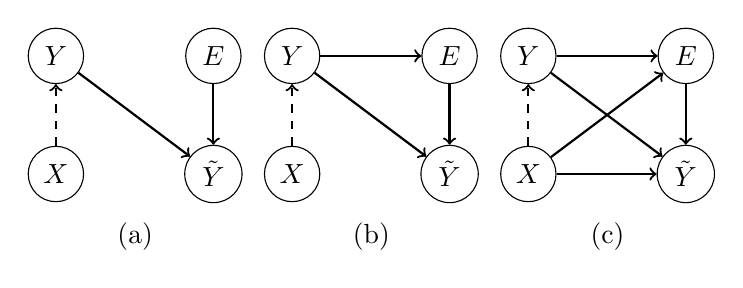
\begin{tikzpicture}[main_node/.style={circle,draw,minimum size=2em,inner sep=3pt]}]

     \node[main_node] (1) at (-1, 0) {$Y$};
     \node[main_node] (2) at (-1, -1.5)  {$X$};
     \node[main_node] (3) at (1, -1.5) {$\tilde{Y}$};
     \node[main_node] (4) at (1, 0) {$E$};
     \path[->,draw,thick]
     (1) edge node {} (3)
     (4) edge node {} (3)
     ;

     \path[->,dashed,thick]
     (2) edge node {} (1)
     ;

     \node[below=2cm] at (current bounding box.base) {(a)};

     \begin{scope}[xshift=3cm,grow=right,baseline]

     \node[main_node] (1) at (-1, 0) {$Y$};
     \node[main_node] (2) at (-1, -1.5)  {$X$};
     \node[main_node] (3) at (1, -1.5) {$\tilde{Y}$};
     \node[main_node] (4) at (1, 0) {$E$};

     \path[->,draw,thick]
     (1) edge node {} (3)
     (4) edge node {} (3)
     (1) edge node {} (4)
     ;

     \path[->,dashed,thick]
     (2) edge node {} (1)
     ;

     \node[below=2cm,xshift=1.5cm] at (current bounding box.base) {(b)};

     \end{scope}

     \begin{scope}[xshift=6cm,grow=right,baseline]
     \node[main_node] (1) at (-1, 0) {$Y$};
     \node[main_node] (2) at (-1, -1.5)  {$X$};
     \node[main_node] (3) at (1, -1.5) {$\tilde{Y}$};
     \node[main_node] (4) at (1, 0) {$E$};

     \path[->, draw,thick]
     (1) edge node {} (3)
     (4) edge node {} (3)
     (1) edge node {} (4)
     (2) edge node {} (3)
     (2) edge node {} (4)
     ;

     \path[->,dashed,thick]
     (2) edge node {} (1)
     ;

     \node[below=2cm,xshift=3cm] at (current bounding box.base) {(c)};

     \end{scope}
 \end{tikzpicture}
 }
 \end{figure}

Many label noise robustness methods can be found on literature, in this work we highlight the \textit{backward} and \textit{forward} loss corrections, proposed by \cite{Patrini2017} using concepts of loss factorization~\citep{Patrini2016}. Those loss correction techniques considers a NAR label noise, which is described by a transition matrix $T$ such as
\begin{equation}
    T_{i,j} = P(\tilde{Y} = y_j|Y = y_i),
\end{equation}
where $\mathcal{Y} = \{y_1, y_2, \ldots, y_c\}$ is the set of all possible class labels. Transition matrix includes corruption probabilities for every possible label combination, each value represents the probability of one label be corrupted onto another. This matrix is row-stochastic and not necessarily symmetric across the classes.
\begin{equation} \label{eq:backward}
    \ell^{\leftarrow}(P(\tilde{Y}|X)) = T^{-1} \ell(P(\tilde{Y}|X))
\end{equation}

The backward loss correction is defined by Equation~\ref{eq:backward} to an arbitrary loss function $\ell$ and a transition matrix $T$. The backward loss correction involves a linear combination of the loss values for each observed label, using coefficients that depends on the probability that each observed label reflects the true class. Intuitively, we are reweighting the loss according to the noise probabilities of each label using the inverse of T and thus somehow going one step back, reverting the noise effects. This corrected loss is unbiased and can be minimized with any conventional back-propagation algorithm, making it flexible to include within different training techniques and data pipelines.
\begin{equation} \label{eq:forward}
    \ell^{\rightarrow}(P(\tilde{Y}|X)) = \ell(T^{\top} P(\tilde{Y}|X))
\end{equation}

However, backward correction requires matrix inversion, which may not exist or may lead to numerical instabilities if the transition matrix T is ill-conditioned. Although there is possible solutions to a bad condition number of T, one should consider using the forward correction, a backward variation proposed by \cite{Patrini2017} to avoid this issue, as defined in Equation~\ref{eq:forward}. While backward acts on the loss itself, forward corrects model predictions. Forward correction does not have the same theoretical guarantees as backward, but offers a label noise robustness, ensuring that the learned model is the minimize over the clean distribution without the need of matrix inversion.

Now we discuss classification methodologies that operate in the presence of label noise. While our research does not directly tackle fairness problems in the presence of label noise, we highlight relevant works that, akin to ours, bridge the domains of fairness and noise in machine learning research.

Some recent works deal with fairness problems in the presence of noise. For example, the sensitive attribute available could be noisy, which could distort the effects of fairness intervention. In this context, \cite{Lamy2019} uses noise-rate estimators from the label noise literature to change a fairness model. Also, \cite{Fogliato2020} proposes a framework for assessing how assumptions on the noise across groups affect the predictive bias properties in risk assessment models. Furthermore, \cite{Wang2020} considers the consequences of naively relying on noisy protected group labels while proposing two new optimization approaches with sensitive attribute noise robustness. A denoised version of the selection problem to deal with noisy sensitive attributes is proposed in \cite{Mehrotra2021}. Lastly, \cite{Celis2021} proposes an optimization framework for classification in the presence of noisy protected attributes.

There is also the perspective of dealing with the proxy features divergence or covariance. A theoretical approach to this issue identifying potential sources of errors can be found in \cite{Prost2021}. The problem of measuring group fairness in ranking based on divergence with proxy features is investigated by \cite{Ghazimatin2022}. A framework of fair semi-supervised learning in the pre-processing phase can be found in \cite{Zhang2022}, which includes predicting labels for unlabeled data, a resampling method, and ensemble learning to improve accuracy and decrease discrimination.

Another research direction is considering how fair models perform in the presence of NNAR label noise, where error rates of corruption depend both on the label class and the membership of a protected subgroup. In this scenario \cite{Wang2021} addresses the problem of fair classification and \cite{Wu2022} provides a general framework for rewriting the classification risk and the fairness metric in terms of noisy data and thereby building robust classifiers. In \cite{Ghosh2023} a study about the presence of noise in the protected attribute can be found.

Furthermore, many recent works deals with fairness under semi-supervised settings considering censored data, that is, for some individuals the class label is not available due censorship~\cite{WZhang2022,WZhang2023_a,WZhang2023_b,WZhang2023_c}. In this scenario, the main approach is to use some technique to estimate the missing data instead of removing the instance from training data. This is closely related to the previous problems of fair learning under noisy data. In censored fairness problems noise can be interpreted as a kind of censorship, as the original data affected by noise is not available.

Bias and noise are two related phenomena, both corrupt data affecting models trained with this data. For example, if noise disproportionately affects different groups this potentially produces unfairness in models that uses this data in training~\citep{Wang2021}. For example, we could have positive true class ($Y = 1$) flipped into negative labels ($\tilde{Y} =0$) more frequently in the protected group ($A = 1$) than in privileged group ($A = 0$). Simultaneously, the negative class ($Y = 0$) could be more frequently flipped into positives observed labels ($\tilde{Y} = 1$) within privileged/unprotected group ($A = 0$). This scenario could lead to a undetected higher false negative rate to protected group and higher false positive rate to privileged group. In this case the Noisy Not at Random data would be a source of negative social bias.

As refered before, in \cite{Mehrabi2019} a non-exhaustive list of bias types was presented. In the scenario described above, the incorrect measurement of the true class resulted in a different observed label ($Y \neq \tilde{Y}$), which could be classified as a \textit{Measurement Bias}. Similarly, a Noisy Not at Random data could lead to a \textit{Population Bias}, where the characteristics of the population represented in the data differ from those of the original target population.

It can be challenging to distinguish between label noise and bias in certain scenarios, specially when noise disproportionately affects different social groups. Although there is some overlapping, they are distinct phenomena. Label noise is a stochastic process that is considered independent and unintentional~\citep{Frenay2014}, whereas bias is rooted in historical and social issues and could be intentional. Furthermore, even noise-free data, correctly represented by observed features and labels, may be unfair since the social phenomena that produce this data could be biased against some groups.

Previous studies on fair machine learning have largely concentrated on understanding how noisy or censored data affects fair learning and on mitigating these effects. Thus, the objective of this work is not to theoretically deal with fair machine learning as a label noise problem or incorporate noisy classes or attributes in fairness problems. In contrast, our approach is inspired by label noise techniques, but with a distinct goal: not merely to analyze or mitigate the impact of noise or censorship, but to directly address and reduce unfairness itself.

\section{Proposal} \label{sec:proposal}

We propose a novel fair classification method inspired by techniques used for classification in the presence of label noise. By using some features of label noise methods that redistribute probabilities for unbalanced noise across classes, our approach re-weights prediction probabilities to reduce disparities in favorable and unfavorable outcomes across social groups.

Whereas forward loss correction~\citep{Patrini2017} uses a transition matrix with corruption probabilities for every label combination in the case of NAR, fair classification problems are more related to NNAR. While forward loss correction uses a transition matrix with corruption probabilities for each label combination, as in the case of NAR, fair classification problems align more with NNAR scenarios. In NNAR, the probability of corruption depends not only on the true class but also on features, analogous to how bias in fairness problems is directed against certain groups. Here our correction does not revert a random label corruption from the true class, but a potentially unfair prediction. While noise label techniques, like forward~\citep{Patrini2017}, aims to correct the prediction targeting a unknown true class using the available noisy label, analogously the proposed technique focus on correcting predictions chasing the unknown fair class using the available unfair label. Despite those are distinct phenomena, the corrections works the same way, adjusting the probabilities of predictions produced by a machine learning model during the training. 

Thus, our proposal is a prediction probability loss reweighting technique that accounts different rates to each group of the sensitive feature, instead of using the same correction to every individual. A correction method that incorporates different probabilities for protected and unprotected groups could be more effective in mitigating bias during the learning phase. Specifically, we want a forward-based correction that takes into account a different matrix to each group of sensitive features, not only one transition matrix as used in label noise techniques. In this scenario, each group of sensitive feature have its own correction, with its own rates for each class combination. Ideally, if we can find an appropriate transition matrix that describes the bias to each group in a specific problem, we can apply a correction that attenuates those negative effects by reweighting model's predictions in the learning process.

Next, we formally present Fair Transition Loss. For purpose of clarity we follow the same structure available at \citep{Patrini2017}, with the pertinent changes to our scope. The Fairness Transition Matrix $T_a$ is defined with some abuse of notation to the group $A=a$ of the sensitive feature as 
\begin{equation}
    T_{a,i,j} = P(\tilde{Y} = y_j|Y = y_i, A=a),
\end{equation}
where label space $\mathcal{Y} = \{y_1, y_2, \ldots, y_c\}$, $c$ the number of classes, $Y=y_i$ is the unknown fair class and $\tilde{Y}=y_j$ is the available and 
possibly unfair label. Here, $T_{a,i,j}$ is the probability of the fair class $Y=y_i$ being unfairly labeled as $\tilde{Y}=y_j$ to an individual of the group $A=a$ due negative social bias. Therefore, suppose that there is an inversible link function $\psi : \Delta^{c-1} \rightarrow \mathbb{R}^c$, where $\Delta^{c-1} \subset [0,1]^c$ is the $c$-simplex, the simplex in a $c$-dimensional space. Thus, a composite loss function, denoted by $\ell_{\psi} : \mathcal{Y} \times \mathbb{R}^c \rightarrow \mathbb{R}$ if it can be written as a decomposition of $\psi^{-1}$, that is,

\begin{equation}
    \ell_{\psi}(Y, h(X)) = \ell(Y, \psi^{-1}(h(X)), 
\end{equation}
where $h:\mathcal{X} \rightarrow \mathbb{R}^c$ is a standard artificial neural network with multiple layers using activation functions, and $h(X)$ is the output o this neural network to a given input $X$. For example, to cross entropy loss function the softmax is the inverse link function. Proper loss functions are those that can be directly used to estimate class probabilities. The minimizer of a proper composite loss has the particular form of the link function applied to the conditional class probabilities $P(Y|X)$. Adding a new conditioning to this formulation, to an individual from group $A=a$ we have

\begin{equation} \label{eq:argmin_ftl}
    \argmin\limits_{h}\mathbb{E}_{X,Y}\ell_{\psi}(Y, h(X|A=a)) = \psi(P(Y|X,A=a)).
\end{equation}

Fair Transition Loss consists in correcting model's predictions with the same technique as forward, but taking into account the sensitive attribute value when choosing the transition matrix. In Theorem~\ref{theorem:ftl} the Fair Transition Loss is formally defined, with a guarantee about its minimizers.

\begin{theorem}\label{theorem:ftl}
    Suppose that the Fairness Transition Matrix $T_a$ for a given sensitive attribute $A=a$ is non-singular. Given a proper composite loss $\ell_{\psi}$, define the Fair Transition Loss as
    \[\FTL_{\psi}(h(X|A=a)) = \ell(T^{\top}_a \psi^{-1}(h(X|A=a))).\]
    Then, the minimizer of the corrected loss under the unfair distribution is the same as the minimizer of the original loss under the fair distribution:
    \[  \argmin\limits_{h}\mathbb{E}_{X,\tilde{Y}}\FTL{\psi}(Y, h(X|A=a)) = \argmin\limits_{h}\mathbb{E}_{X,Y}\ell_{\psi}(Y, h(X|A=a)).\]
\end{theorem}
\begin{proof}
    First notice that:
    \begin{align} \label{eq:proof_ftl}
        \FTL_{\psi}(Y, h(X|A=a)) &= \ell(Y, T^{\top}_a \psi^{-1}(h(X|A=a))) \nonumber \\
        &= \ell_{\phi}(Y, h(X|A=a)),
    \end{align}
    where we denote $\phi^{-1} = \psi^{-1} \circ T_a^{\top}$. Equivalently, $\phi = (T_a^{-1})^{\top} \circ \psi$ is invertible by composition of invertible functions, its domain is $\Delta^{c-1}$ as of $\psi$ and its codomain is $\mathbb{R}^{c}$. The last loss in Equation~\ref{eq:proof_ftl} is proper composite with link $\phi$. Finally, from Equation~\ref{eq:argmin_ftl}, the loss minimizer over the unfair distribution is
    \begin{align}
        \argmin\limits_{h}\mathbb{E}_{X,\tilde{Y}}\ell_{\phi}(Y, h(X|A=a)) &= \phi(P(\tilde{Y}|X,A=a)) \\
        &= \psi((T_a^{-1})^{\top}) P(\tilde{Y}|X,A=a) \\
        &= \psi(P(Y|X,A=a)),
    \end{align}
    that proves the Theorem by Equation~\ref{eq:argmin_ftl} once again.
\end{proof}

Considering a common scenario with only two groups in sensitive attributes (protected and privileged), we can correct the model's predictions using two different fair transition matrices. One with rates applied while learning instances from the protected group, and the other with rates applied while learning instances from the privileged group. Formally, to the sensitive feature $A \in \{0,1\}$, let $T_0$ the transition matrix associated with privileged/unprotected group ($A = 0$) and $T_1$ with the protected group ($A = 1$), $\FTL$ can be computed as

\begin{equation}
    \FTL(P(\tilde{Y}|X)) = (1-A) \cdot \ell(T^{\top}_0 P(\tilde{Y}|X)) + A \cdot \ell(T^{\top}_1 P(\tilde{Y}|X)),
\end{equation}
which in a standard batch learning, consists in alternating the transition matrix applied according instance's sensitive attribute.

Furthermore, to a common binary classification problem, where there is a positive (favorable) class and a negative (unfavorable) class, and two groups from sensitive feature (protected and privileged), we have two $2\times2$ transition matrices. Intuitively we are choosing rates to increase or decrease the probability of each group to be classified with the positive or negative prediction. We name those rates associated with increasing the probability to achieve the positive outcome as \textit{promotion} rate, and those associated with increasing the probability to receive the negative outcome as \textit{demotion} rate. As the transition matrix is row-stochastic, we can describe $T_0$ and $T_1$ as
\begin{equation} \label{eq:transition_matrices}
    T_0 = \left[\begin{array}{cc}
        1-d_0 & d_0\\
        p_0 & 1-p_0\\
    \end{array}\right],\;
    T_1 = \left[\begin{array}{cc}
        1-d_1 & d_1\\
        p_1 & 1-p_1\\
    \end{array}\right],
\end{equation}
where $d_0$ is the privileged demotion rate, $p_0$ the privileged promotion rate, the $d_1$ protected demotion rate, and $p_1$ the protected promotion rate. With an appropriate combination of $d_0$, $p_0$, $d_1$, $p_1$ we can define a transition matrix pair that should be able to reweight model's predictions with $FTL$ to achieve fairer results with a reasonable model performance. The central problem in our methodology thus relies in choosing these rates, which can be seen as an hyperparameter optimization problem.

Our hyperparameter optimization problem consists in finding an optimal trade-off between fairness and performance, which can be described as a MOO problem, as defined in Equation~\ref{def:moo}. Here, the hyperparameter configuration is $\lambda = (d_0, p_0, d_1, p_1)$. Since the transition matrix is row stochastic these parameters are sufficient to define $T_0$ and $T_1$. We want to maximize model performance $\rho(\lambda)$ and minimize fairness metric $\varphi(\lambda)$. 

\begin{equation} \label{eq:obj_fn}
    G(\lambda) = \rho(\lambda) - \varphi(\lambda).
\end{equation}

Following some MOO approaches to fair machine learning, we will use a linear scalarization setup to define the optimization metric~\citep{Schmucker2020,Petrovic2021}. As we yet have four hyperparameter to fine-tune, and in \cite{Cruz2021} the relative importance $\alpha$ is fixed at $0.5$, we choose a simple and intuitive objective function in Equation~\ref{eq:obj_fn} to maximize without the parameter $\alpha$, i.e., giving same importance to fairness and performance. In Equation~\ref{eq:obj_fn} we establish a simple objective to optimize, but one might need to consider a different formulation depending on the specific problem at hand.


\section{Experimental setup} \label{sec:experimental}

In this section, we detail the experimental setup employed to benchmark our model against relevant in-processing fair classification models found in standard fairness toolkits, namely, Prejudice Remover~\citep{Kamishima2012}, Adversarial Debiasing~\citep{Zhang2018}, and Gerry Fair Classifier~\citep{kearns18a}. We use the implementation of these methods from AI Fairness 360 toolkit~\citep{aif360-oct-2018}. The baseline is a Standard MLP using two hidden layers with $100$ hidden units each, $ReLU$ activation function, batch size of $64$, $50$ epochs early stopped at $3$ epochs without improvement~\citep{Li2020} and softmax in output, trained with ADAM optimizer~\citep{KingmaB14} with learning rate at $3\mathrm{e}{-4}$. The only difference between baseline MLP and Fair Transition Loss MLP is that baseline uses standard Binary Cross Entropy Loss. The Gerry Fair Classifier implementation uses the False Negative Rate as its fairness definition and in Adversarial Debiasing classifier the hidden size is $100$ units. Additionally, we compare the Fair Transition Loss within the Adaptive Priority Reweighting~\cite{HuXT23}, a promising fairness promoting technique focused on improving generalization, which outperformed many recent methods such as \cite{jiang2020identifying}, \cite{mroueh2021fair}, and \cite{roh2020fairbatch}.

Our methodology consists of two phases: hyperparameter tuning and testing. In the hyperparameter tuning phase we perform a Bandit-Based pruning approach using HyperBand~\citep{Li2018} with Tree-structured Parzen Estimator Sampler (TPE)~\citep{bergstra2011} over 100 trials. Those techniques achieves better solutions to multi-objective hyperparameter optimization in the same number of trials than conventional approaches like Grid Search and Random Search~\citep{Morales-Hernandez2023}. At each trial fitness function is evaluated by performing a complete training and validation, where both model performance and fairness metrics are assessed. The fitness function is computed based on the objective defined in Equation~\ref{eq:obj_fn}. This same experimental procedure can be adapted to utilize other hyperparameter tuning algorithms such as FairRandom Search, Fair TPE, and Fairband~\citep{Cruz2021}.

Once the best hyperparameters are selected, we proceed to the testing phase, where a new training is conducted using those optimal hyperparameters. After this training, we evaluate the model's performance on a separate test set that was not used during the hyperparameter tuning phase, which are reported. This complete tuning-training-testing described is repeated $15$ times with dataset re-sampling then we proceed to comparison. Here the re-sampling consists in shuffling the whole dataset before splitting, which is better described further in this section.

As the objective defined in Equation~\ref{eq:obj_fn} can be achieved with different performance and fairness metrics, we compare the proposed method with other relevant in-processing techniques from literature in different optimization scenarios. In addition to Accuracy (Acc.) as performance metric, we also evaluate the Mathews Correlation Coefficient (MCC), which has advantages over F1 score and Accuracy in binary classification evaluation~\citep{chicco2020advantages}. To this performance metric, $1$ means a perfect prediction according true class, $-1$ a complete inversion and $0$ an average random outcome. As fairness metric we consider Statistical Parity (Stat. Parity, Definition~\ref{def:demo_parity}), Equal Opportunity (Eq. Opp., Definition~\ref{def:eq_opp}) and Equalized Odds (Eq. Odds, Definition~\ref{def:eq_odds}). Thus we have the following optimization scenarios: MCC and Statistical Parity; MCC and Equal Opportunity; MCC and Equalized Odds; Accuracy and Statistical Parity; Accuracy and Equal Opportunity; Accuracy and Equalized Odds.

\begin{table}[ht]
\centering
\caption{Hyperparameters search ranges or options of each method.}\label{tab:hyperparameters}
{\footnotesize
\begin{tabular}{lll}
\toprule
Method & Parameter & Range/options \\ \midrule
 Standard MLP (baseline) & dropout & $[0.0,\,0.2]$  \vspace{1ex} \\
 Prejudice Remover~\citep{Kamishima2012} & $\eta$ & $[0.0,\,50.0]$ \vspace{1ex} \\
 Adversarial Debasing~\citep{Zhang2018}& $\alpha$ & $[0.0,\,1.0]$  \vspace{1ex} \\
 Gerry Fair Classifier~\citep{kearns18a} & $C$ & $[0.0,\,20.0]$ \\
 &  $\gamma$ & $\{0.1,\,0.01,\,0.001\}$ \vspace{1ex} \\
 Adaptive Priority Reweighting~~\citep{HuXT23} & $\alpha$ & $[0.0,\,10000.0]$ \\
 &  $\eta$ & $[0.5, 3.0]$ \vspace{1ex} \\
 Fair Transition Loss & $d_0,p_0,d_1,p_1$ & $[0.0,\,1.0]$ \\
 &  dropout & $[0.0,\,0.2]$ \\
\bottomrule
\end{tabular}
}
\end{table}

Table~\ref{tab:hyperparameters} presents the methods hyperparameters along with their corresponding search ranges or options. While each method may possess a varying number of hyperparameters and range sizes, all are optimized under the same conditions and number of configurations to guarantee a balanced comparison. In Figure~\ref{fig:fitness_sensibility} we present a brief sensibility analysis on the fitness functions with different fairness and performance values over those six optimization scenarios listed before. Here we perform a complete hyperparameter tuning with HyperBand and TPE over $100$ trials using the baseline model (Standard MLP) with the Adult Income dataset optimizing the hyperparamers reported on Table~\ref{tab:hyperparameters}. This sensibility analysis aims better present the linear objective function behavior within performance and fairness metrics evaluated in this study.

\begin{figure}[!ht]
\centering
\caption{Sensibility analysis on optimized fitness functions within different performance and fairness metrics. Results from complete hyperparameter tuning through $100$ trials with baseline model over the Adult Income dataset.}
    \label{fig:fitness_sensibility}
    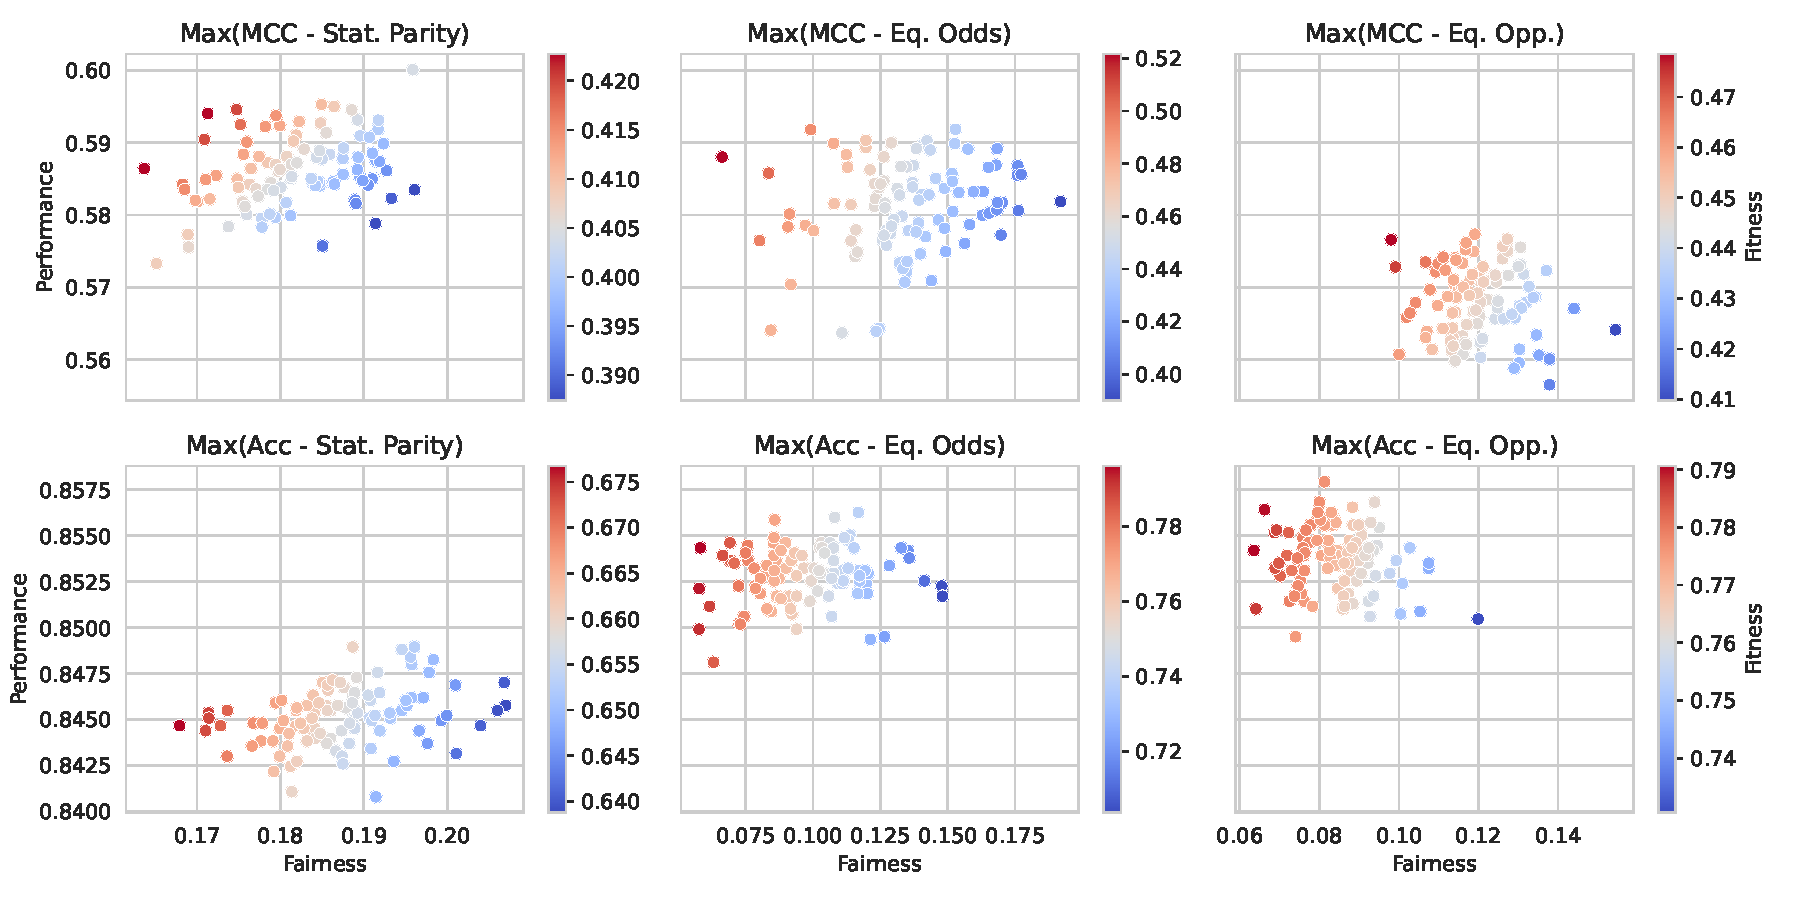
\includegraphics[width=1\linewidth]{images/fitness_sensibility.pdf}
\end{figure}

Each plot in Figure~\ref{fig:fitness_sensibility} illustrates the fitness value corresponding to specific performance and fairness metrics. The color scheme in the plots represents the fitness values, with higher values in red and lower values in blue. On the $x$-axis, we have the fairness metric, where a lower value is preferable. The $y$-axis represents the performance metric, with higher values being preferred. The color gradient in these plots demonstrates the linear relationship between fitness and variations in the corresponding performance and fairness metrics. It is important to note that the scale of the fairness metric is significantly smaller than that of the performance metric. However, it is sufficiently to act as a penalization. The general fitness function in the scenarios described is capable of producing results with reduced bias while maintaining similar performance levels. Although each metric combination has different scales, each hyperparameter tuning experiment uses only one metric combination at a time, ensuring consistency in the optimization process.

On these plots we used the fitness and performance levels obtained through the TPE sampler with HyperBand pruning during the hyperparameter tuning phase using the baseline model, as previously described. In this setting, the solution (i.e., the combination of hyperparameters) that yields the best fitness value is selected for a new complete training phase. This involves assessing metrics on test data not used in the previous phase. To ensure robust evaluation, the dataset is reshuffled, re-split into train, validation and test segments, and this entire process is repeated over 15 iterations.

To properly compare this set of $15$ results of each method, we conduct an Almost Stochastic Order (ASO) test \citep{dror2019deep}, which is a significance test suitable for comparing complex machine learning models with various hyperparameters. The ASO test involves evaluating a set of metrics through multiple samplings of a Collection of Statistics (in this case assessed in test phase using random resampling) to compare one method against another. The $ASO(A, B)$ function yields a value in the range $[0, 1]$, given two methods $A$ and $B$. If $ASO(A, B)$ is lesser than $0.5$, we can reject the null hypothesis and conclude that method $A$ outperforms method $B$ in the given task. That is, method $A$ produces stochastically larger values than method $B$ for a given metric. The lower the $ASO(A, B)$ value, the stronger the evidence that $A$ is superior to $B$ in that particular task, which can be interpreted as a confidence interval. Therefore, we perform pairwise comparisons between all methods for each optimization scenario outlined previously and for each dataset.

%\subsection{Datasets description}\label{sec:datasets}

Our experiments uses common datasets used in Fair Classification problems, namely \textit{Adult Income}~\citep{misc_adult_2}, \textit{German Credit}~\citep{misc_statlog_(german_credit_data)_144}, \textit{Bank Marketing}~\citep{misc_bank_marketing_222}, and \textit{COMPAS Recidivism}~\citep{misc_compas}. We use the dataset readers available in the AI Fairness 360 toolkit~\citep{aif360-oct-2018} with its standard configurations. Instances with missing data are removed.

\begin{table}[ht]
    \centering
    \caption{Dataset details used in this work, including performance and fairness metrics assessed to a standard classifier without tuning, and the maximum correlation between sensitive feature and the other features.}\label{tab:datasets}
    {\footnotesize
    \begin{tabular}{lrrrr}
        \toprule
        \multirow{2}{*}{\shortstack[l]{Dataset}} & \multirow{2}{*}{\footnotesize\shortstack[l]{Adult\\ Income}} & \multirow{2}{*}{\footnotesize\shortstack[l]{Bank\\ Marketing}} & \multirow{2}{*}{\footnotesize\shortstack[l]{COMPAS\\ Recidivsm}} & \multirow{2}{*}{\footnotesize\shortstack[l]{German\\ Credit}} \\ \\
        \midrule
\# Features & 102 & 57 & 401 & 58 \\
\# Instances & 45222 & 30488 & 6167 & 1000 \\
Sensitive Attribute & sex & age & race & sex \\
Positives & 24.78\% & 12.66\% & 54.45\% & 70.00\% \\
Negatives & 75.22\% & 87.34\% & 45.55\% & 30.00\% \\
Privileged & 67.50\% & 97.17\% & 34.05\% & 69.00\% \\
Unprivileged & 32.50\% & 2.83\% & 65.95\% & 31.00\% \\
Accuracy & 0.846 & 0.906 & 0.358 & 0.685 \\
MCC & 0.572 & 0.553 & -0.275 & 0.000 \\
Stat. Parity. & 0.192 & 0.106 & 0.172 & 0.074 \\
Equal Opportunity & 0.094 & 0.145 & 0.120 & 0.043 \\
Equalized Odds & 0.092 & 0.094 & 0.163 & 0.122 \\
Maximum Correlation & 0.527 & 0.364 & 0.826 & 0.593 \\
        \bottomrule
    \end{tabular}
    }
\end{table}


Table~\ref{tab:datasets} present dataset details used in this work, including the number of features before pre-processing, the count of valid instances, the proportion of positive and negative labels, the sensitive feature considered in experiments, the proportion of privileged and unprivileged groups within the corresponding sensitive feature, reference performance and fairness metrics using a standard Random Forest Classifier with $1000$ classifiers without tuning, and the maximum correlation coefficient between the sensitive feature and the other features. The maximum correlation is useful to assess whether it is possible to use another feature as proxy to the sensitive feature, which is commonly referred as redlining effect~\citep{Pedreschi2008}.

The \textit{Adult Income} dataset presents a classification task to predict whether an individual earns more than $50,000$ per year. This dataset consists of $48,842$ instances sourced from the U.S. 1994 Census database. The sensitive attribute used in this task is sex, with the male group considered privileged and the female group protected (unprivileged). In the \textit{German Credit} dataset, the task consists of classifying $1,000$ individuals described by a set of attributes as good or bad credit risks. Similar to the \textit{Adult Income} dataset, here we use sex as the sensitive attribute, with the male group considered privileged and the female group protected. The \textit{Bank Marketing} classification task aims to predict whether $45,211$ clients will subscribe to a term deposit after direct marketing campaigns (phone calls) by a Portuguese banking institution. In this case, the sensitive feature is age, where individuals under the age of $25$ are considered unprivileged, while those aged $25$ and older are considered privileged. The \textit{COMPAS} dataset presents around $80,000$ criminal records from the Broward County Clerk’s Office. The task here is to predict whether a defendant will recidivate in the next two years. The sensitive feature in this case is race, with Caucasians as the privileged group and non-Caucasians (Black and Hispanic) as unprivileged.

For all datasets, the data preparation process is the same, one-hot encoding for categorical features and standardize the numerical features. We perform a random split, with $80\%$ allocated for the hyperparameter tuning phase and the remaining $20\%$ reserved for evaluating metrics in the test phase. Within the hyperparameter tuning phase, this corresponding fraction of data is further randomly split, with $80\%$ assigned to training and $20\%$ to validation. The validation set allows us to assess metrics and compute the fitness function for each hyperparameter configuration. In datasets where there is originally some kind of split (e.g., train set and test set in separate files), all available data is merged and then shuffled to produce new splits at each run.

\section{Results and discussion} \label{sec:results}

This section summarizes our results, comparing Fair Transition Loss (FTL) with the baseline Standard MLP (MLP) and some relevant fair in-processing methods: Adversarial Debiasing (AD), Prejudice Remover (PR), Gerry Fair Classifier (GFC) and Adaptive Priority Reweighting (APW).

\begin{table}[ht]
    \centering
    \caption{Almost Stochastic Order test comparing Fair Transition Loss fitness. Values under $0.5$ (in bold) mean that FTL outperforms corresponding method in such optimization scenario.} \label{tab:aso_compare}
    {\footnotesize
    \begin{tabular}{llccccc}
    \toprule
     \multirow{2}{*}{\shortstack[l]{Fairness/Performance\\Metric}} & Dataset & MLP & AD & PR & GFC & APW \\ \\
\midrule
\multirow{4}{*}{\shortstack[l]{Statistical Parity\\MCC}} & Adult Income & \textbf{0.00} & \textbf{0.15} & 1.00 & \textbf{0.00} & 1.00 \\
 & Bank Marketing & \textbf{0.01} & \textbf{0.00} & \textbf{0.00} & \textbf{0.00} & \textbf{0.00} \\
 & Compas Recidivism & \textbf{0.01} & \textbf{0.25} & \textbf{0.00} & \textbf{0.02} & \textbf{0.00} \\
 & German Credit & \textbf{0.28} & \textbf{0.30} & \textbf{0.39} & \textbf{0.21} & \textbf{0.28} \vspace{1ex}\\

\multirow{4}{*}{\shortstack[l]{Equal Opportunity\\MCC}}  & Adult Income & \textbf{0.01} & \textbf{0.00} & \textbf{0.05} & \textbf{0.00} & 0.93 \\
 & Bank Marketing & 0.81 & \textbf{0.18} & \textbf{0.24} & \textbf{0.09} & 0.77 \\
 & Compas Recidivism & \textbf{0.00} & 1.00 & \textbf{0.00} & 0.66 & 1.00 \\
 & German Credit & 1.00 & \textbf{0.23} & 0.84 & 0.78 & 0.76 \vspace{1ex}\\

\multirow{4}{*}{\shortstack[l]{Equalized Odds\\MCC}}  & Adult Income & \textbf{0.03} & \textbf{0.28} & \textbf{0.42} & \textbf{0.00} & \textbf{0.00} \\
 & Bank Marketing & \textbf{0.46} & \textbf{0.18} & \textbf{0.12} & \textbf{0.02} & \textbf{0.18} \\
 & Compas Recidivism & \textbf{0.01} & 0.58 & \textbf{0.00} & \textbf{0.07} & \textbf{0.00} \\
 & German Credit & 1.00 & \textbf{0.07} & 1.00 & \textbf{0.31} & 1.00 \\
\midrule
\multirow{4}{*}{\shortstack[l]{Statistical Parity\\Accuracy}}  & Adult Income & \textbf{0.01} & \textbf{0.26} & \textbf{0.32} & \textbf{0.00} & 0.53 \\
 & Bank Marketing & \textbf{0.25} & 1.00 & 1.00 & 0.76 & 0.82 \\
 & Compas Recidivism & \textbf{0.00} & 1.00 & \textbf{0.10} & 1.00 & \textbf{0.00} \\
 & German Credit & 1.00 & \textbf{0.26} & 1.00 & 1.00 & 1.00 \vspace{1ex}\\

\multirow{4}{*}{\shortstack[l]{Equal Opportunity\\Accuracy}} & Adult Income & 0.89 & 0.97 & 1.00 & \textbf{0.23} & 0.98 \\
 & Bank Marketing & 1.00 & \textbf{0.39} & 0.81 & 1.00 & 1.00 \\
 & Compas Recidivism & \textbf{0.01} & 0.78 & \textbf{0.00} & \textbf{0.10} & 1.00 \\
 & German Credit & 1.00 & 0.64 & 1.00 & 1.00 & 1.00 \vspace{1ex}\\

\multirow{4}{*}{\shortstack[l]{Equalized Odds\\Accuracy}} & Adult Income & \textbf{0.01} & \textbf{0.21} & \textbf{0.19} & \textbf{0.00} & 1.00 \\
 & Bank Marketing & 0.76 & \textbf{0.40} & 0.82 & 1.00 & 1.00 \\
 & Compas Recidivism & \textbf{0.01} & \textbf{0.45} & \textbf{0.00} & \textbf{0.01} & \textbf{0.00} \\
 & German Credit & 1.00 & \textbf{0.12} & 1.00 & 1.00 & 1.00 \\

\bottomrule
\end{tabular}


    }
\end{table}

As we have multiple optimization scenarios with different objective functions and datasets, and to each of them multiple runs, we present in Table~\ref{tab:aso_compare} the results of the ASO test described before, which allow us to properly compare each method to FTL. Values under $0.5$ (in bold) mean that we can reject the null hypothesis, i.e., FTL produces stochastically larger fitness than method in respective column for a objective and dataset. Lower values indicate stronger evidence. The complete results with mean and standard deviation of fitness, performance and fairness can be found in tables~\ref{tab:complete_mcc_parity} to ~\ref{tab:complete_acc_odds} to a fairness-performance trade-off analysis.

In $69$ of $120$ comparison scenarios from Almost Stochastic Order test (Table~\ref{tab:aso_compare}), it is possible to claim that FTL outperforms its competitor, i.e., FTL produces stochastically higher fitness values. Despite these positive results, one can argue that the proposed technique only adds extra hyperparameters that increase models flexibility to achieve higher fitness values. In other words, are we effectively describing bias in datasets by transition matrices as claimed before? To address this, we showcase various FTL hyperparameter combinations selected during the tuning phase described in Section~\ref{sec:experimental}, comparing with corresponding dataset information available at Table~\ref{tab:datasets}. We perform this analysis using \textit{Adult Income} dataset. The corresponding hyperparameters can be found in Table~\ref{tab:found_hyperparameters}. Here, high values mean that FTL alters the corresponding probabilities, while values close to zero indicate minimal interference by the method.

\begin{table}[ht]
    \centering
    \caption{Fair Transition Loss hyperparameters chosen by optimizing different metrics in \textit{Adult Income} dataset.} \label{tab:found_hyperparameters}
    {\footnotesize
    \begin{tabular}{lcccc}
        \toprule
        \multirow{2}{*}{\shortstack[l]{Objective}} & \multirow{2}{*}{\footnotesize\shortstack[c]{$d_0$\\Priv. Dem.}} & \multirow{2}{*}{\footnotesize\shortstack[c]{$p_0$\\Priv. Prom.}} & \multirow{1}{*}{\footnotesize\shortstack[c]{$d_1$\\Prot. Dem.}} & \multirow{2}{*}{\footnotesize\shortstack[c]{$p_1$\\Prot. Prom.}} \\ \\
        \midrule
        MCC and Stat. Parity & 0.056 & 0.076 & 0.043 & 0.878 \\
        MCC and Eq. Opp. & 0.292 & 0.455 & 0.329 & 0.575 \\
        MCC and Eq. Odds & 0.037 & 0.165 & 0.005 & 0.432 \\
        Acc. and Stat. Parity & 0.470 & 0.110 & 0.023 & 0.446 \\
        Acc. and Eq. Opp. & 0.389 & 0.326 & 0.311 & 0.530 \\
        Acc. and Eq. Odds & 0.497 & 0.286 & 0.228 & 0.094 \\
        \bottomrule
    \end{tabular}}
\end{table}


When optimizing for MCC and Statistical Parity, there's a notable high value for protected promotion. This value is compatible with the high corresponding fairness metric for this dataset, approximately $0.19$ without correction. This increases the likelihood that an unprivileged instance receives a favorable outcome. Since statistical parity only compare the probability of a positive outcome across groups (ignoring true class) this is enough. The other hyperparameters presents low values. In contrast to the previous case, optimizing Equal Opportunity requires compatible false negative rates. Optimizing this fairness metric within MCC produces the effect of promoting both privileged and protected, although protected with higher values. This produces the effect of reducing false negatives at all, since the method enhances the probability of a positive outcome. This effect is counterbalanced with intermediate demotion rates to both groups through a finetuning to keep MCC. Note that Equal Opportunity values without correction to this dataset is not as high as Statistical Parity. To optimize Equalized Odds within MCC it is necessary to keep both false negatives and false positives comparable across groups, which lead to a less intense intervention when compared to Equal Opportunity. Here remains the high values to protected promotion to achieve fairness.

There is a remarkable difference between hyperparameters found through optimizing Accuracy and MCC. While MCC handles unbalanced classes effectively, Accuracy only measures the probability of correctly predicting an instance. If the dataset is unbalanced it is possible to achieve high Accuracy only by predicting the label of the more frequent class. In this dataset, only about a quarter of the instances are positives, which can lead to more frequent negative outcomes to achieve higher Accuracy. Results optimizing for Accuracy show significantly higher demotion rates compared to those from MCC optimization, both to privileged and protected groups. From this analysis, it's evident that the proposed methodology effectively describes and mitigates bias in a dataset according to a given fairness definition and while keeping targeted performance metric at a reasonable level.

Now we discuss the results to each objective, starting with MCC and Statistical Parity. To this objective Fair Transition Loss consistently outperforms all methods at all classification tasks, except Prejudice Remover (PR) and Adaptive Priority Reweighting (APW) in \textit{Adult Income}. Figure~\ref{fig:boxplot_mcc_parity} presents a box-plot comparison, where we can see that FTL, PR and APW are effectively drawn. While FTL and APW has little bit higher values, PR presents smaller variance. AS PR is a regularized logistic regression, it is a smaller model than FTL, which can explain the also smaller variance.

\begin{figure}[!ht]
\centering
\caption{Fitness values optimizing MCC and multiple fairness metrics.}
\begin{subfigure}{.32\linewidth}
    \caption{Statistical Parity}
    \label{fig:boxplot_mcc_parity}
    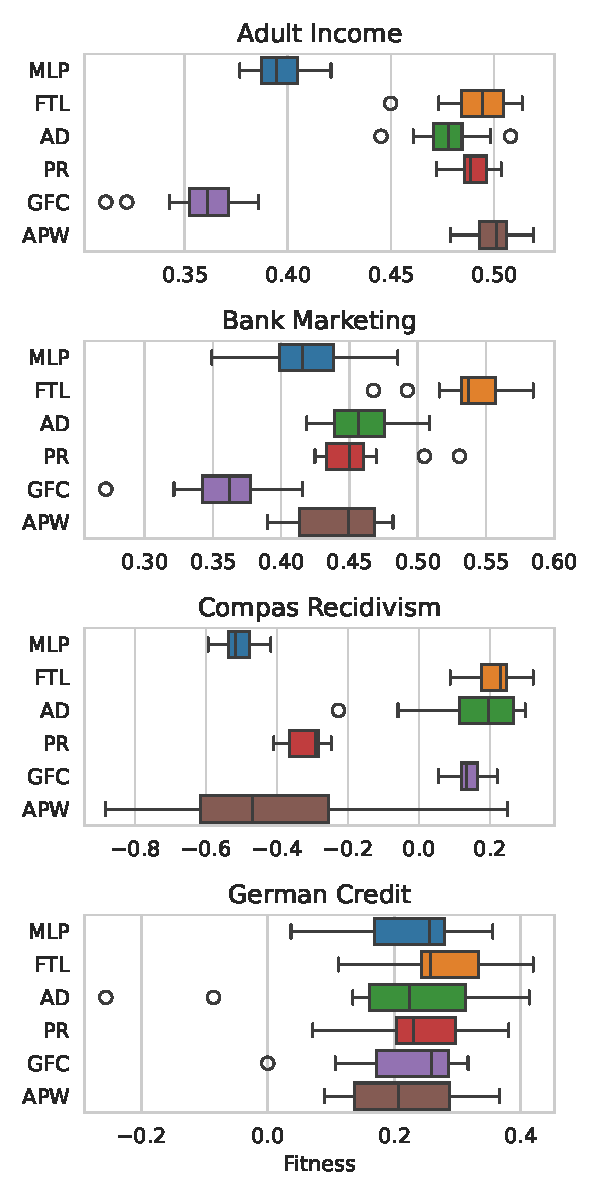
\includegraphics[width=1\linewidth]{images/boxplot_mcc_parity.pdf}
\end{subfigure}
\begin{subfigure}{.32\linewidth}
    \caption{Equal Opportunity}
    \label{fig:boxplot_mcc_opp}
    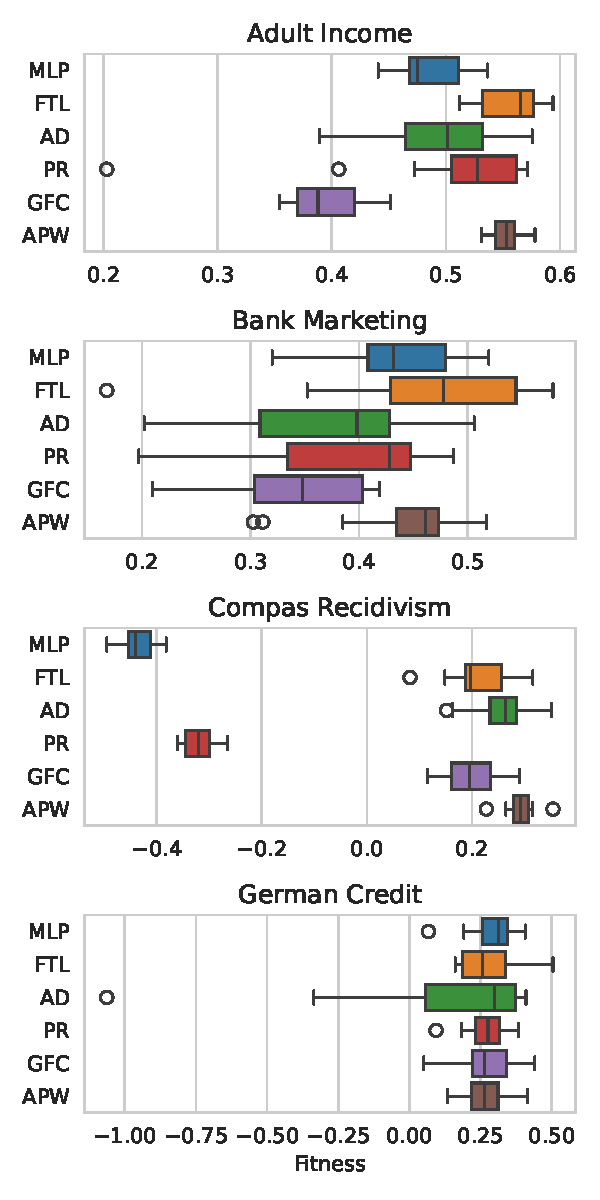
\includegraphics[width=1\linewidth]{images/boxplot_mcc_opportunity.pdf}
\end{subfigure}
\begin{subfigure}{.32\linewidth}
    \caption{Equalized Odds}
    \label{fig:boxplot_mcc_odds}
    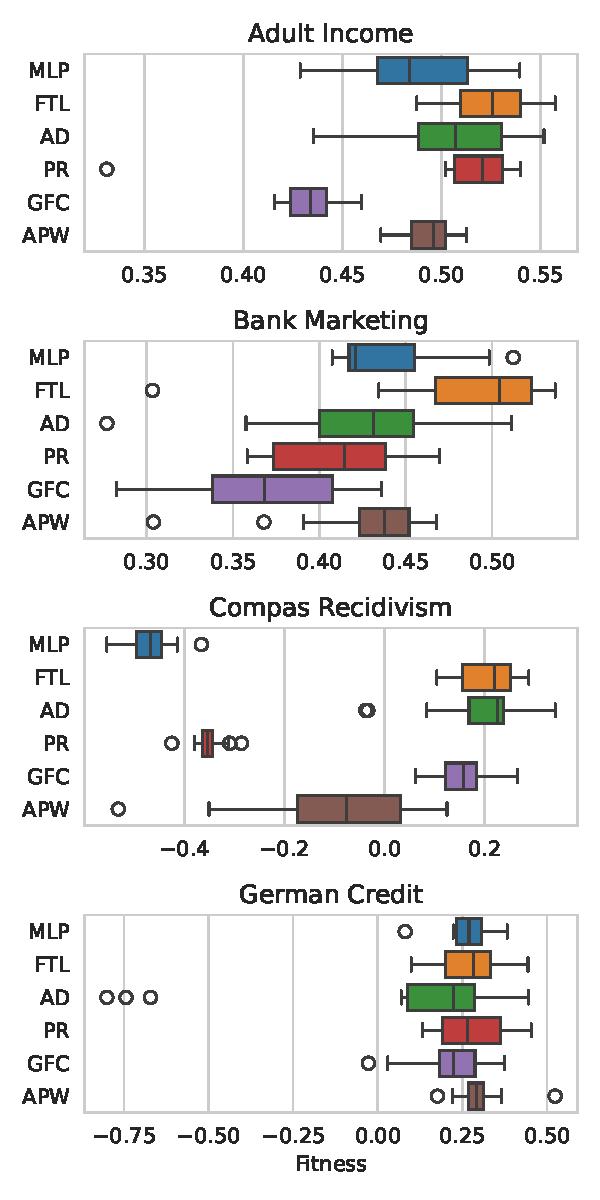
\includegraphics[width=1\linewidth]{images/boxplot_mcc_odds.pdf}
\end{subfigure}
\end{figure}

When comparing the optimization results for MCC and Equal Opportunity, FTL consistently outperforms its counterparts in most scenarios. Here we have only one discrepancy, as APW presents slightly advantage over FTL on \text{COMPAS} dataset. Also, on German Credit dataset all methods achieved similar results. Given the small size of this dataset, we theorize that all methods, barring AD, have reached the Pareto front — meaning, any further improvements in fairness would necessitate a proportional sacrifice in performance. This equilibrium between baseline (MLP), FTL, PR, GFC and APW is evident in Figure~\ref{fig:boxplot_mcc_opp}.

The sub-optimal results of AD can likely be attributed to the dataset's limited size; with merely $1000$ instances, this dataset might be too small for the an adversarial model like AD train effectively. This pattern of AD underperforming persists across subsequent classification tasks involving this dataset. Interestingly, also with the exception of AD, we notice that the variance in results for most optimization scenarios is smaller than in other classification tasks. This observation further underscores our Pareto front hypothesis and suggests that the classification task's simplicity may contribute to the reduced variability in outcomes.

When optimizing for MCC and Equalized Odds, we find that the results are consistent, with FTL outperforming its counterparts in most scenarios. Notably, within the \textit{German Credit} dataset, FTL surpasses not just AD but also GFC. Since GFC primarily relies on the False Negative Rate for its fairness definition, it has a natural advantage when optimizing for Equal Opportunity compared to Equalized Odds, which requires maintaining equitable False Positive and False Negative Rates. As observed in the previous comparisons, Figure~\ref{fig:boxplot_mcc_odds} underscores that the baseline, FTL, PR and APW seem to hit the Pareto front for this dataset.

Upon examining FTL's results when optimizing for MCC across all the fairness metrics evaluated, it's evident that FTL consistently  superior results compared to its counterparts. Specifically, FTL achieves stochastically higher fitness values in $44$ out of the $60$ scenarios evaluated. Given the inherent challenges associated with optimizing MCC compared to Accuracy, we attribute FTL's dominance in the MCC optimization to its capability of effectively capturing the bias idiosyncrasies of the dataset and the specified performance and fairness metrics trough transition matrices.

Furthermore, it's noteworthy that both the baseline and PR models substantially underperform across all optimization scenarios in the \textit{COMPAS Recidivism} classification task. This dataset, characterized by its complexity with $401$ features, might be at the heart of these subpar results. We theorize that the this lack of performance could be due to an insufficiently large model to navigate such a high-dimensional space, especially when we observe, as indicated in Table~\ref{tab:datasets}, that the standard performance on this dataset is relatively low.

When turning our attention to results obtained by optimizing Accuracy, we must first reiterate its inherent simplicity as a performance metric compared to MCC. Given its nature, it allows models to attain high values simply by predicting the label of the predominant class. In such circumstances, it is comparatively easier to reach the Pareto front. Even under these conditions, FTL displays commendable competitiveness. Although it achieves stochastically higher fitness values in $25$ of the $60$ scenarios, this rate is notably less than what we observed when optimizing for MCC. By juxtaposing Figures~\ref{fig:boxplot_acc_parity},~\ref{fig:boxplot_acc_opp},~and~\ref{fig:boxplot_acc_odds} with Table~\ref{tab:aso_compare}, we discern that in scenarios where FTL does not have the upper hand, it still competes closely with its counterparts. This very close results are primarily attributed to multiple methods simultaneously approaching the Pareto front. Likely when optimizing for MCC using Equal Opportunity as fairness metric, APW presents slightly advantage over FTL on \text{COMPAS} dataset.

A particularly straightforward fair classification task emerges when optimizing for Accuracy and Statistical Parity within the \emph{Adult Income} dataset. With this pronounced class imbalance, models can lean into over-predicting the majority class, thereby aligning the probabilities of positive predictions across the groups. This strategy results in a exceptionally low variance across all methodologies. A similar, albeit reduced, effect can be observed within the \textit{German Credit} dataset, as previously highlighted.

\begin{figure}[!ht]
\centering
\caption{Fitness values optimizing Accuracy and multiple fairness metrics.}
\begin{subfigure}{.32\linewidth}
    \caption{Statistical Parity}
    \label{fig:boxplot_acc_parity}
    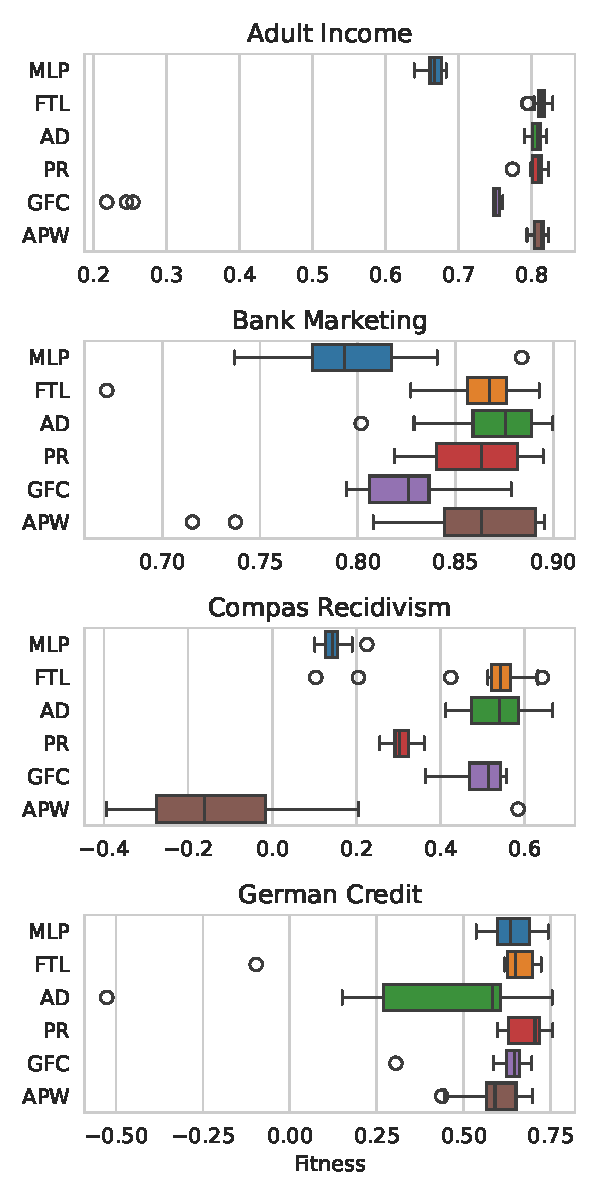
\includegraphics[width=1\linewidth]{images/boxplot_acc_parity.pdf}
\end{subfigure}
\begin{subfigure}{.32\linewidth}
    \caption{Equal Opportunity}
    \label{fig:boxplot_acc_opp}
    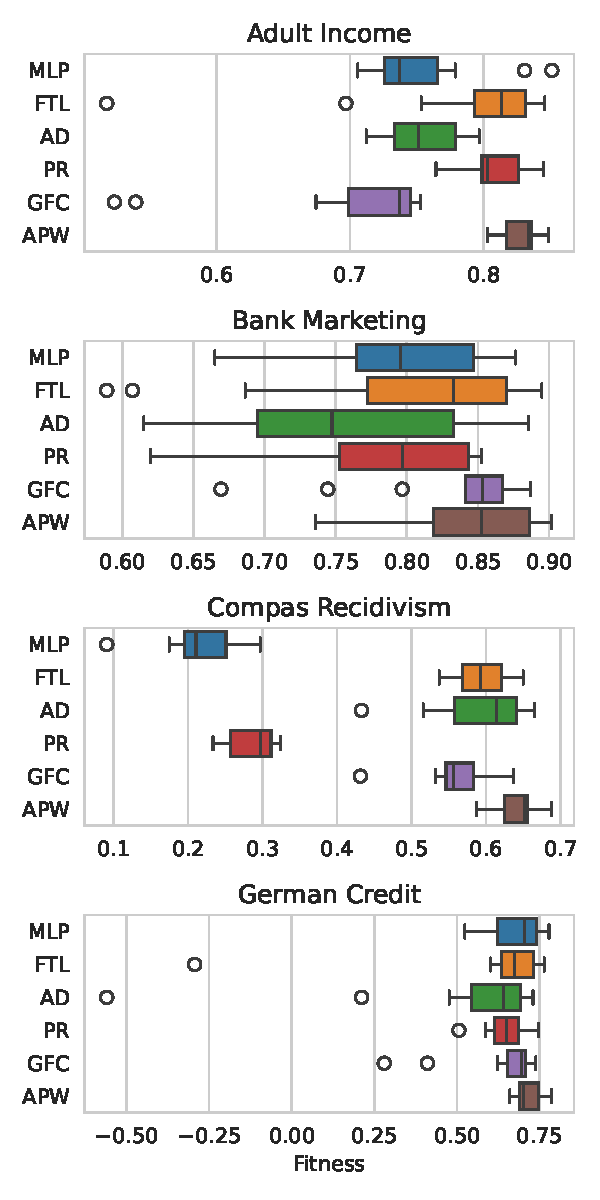
\includegraphics[width=1\linewidth]{images/boxplot_acc_opportunity.pdf}
\end{subfigure}
\begin{subfigure}{.32\linewidth}
    \caption{Equalized Odds}
    \label{fig:boxplot_acc_odds}
    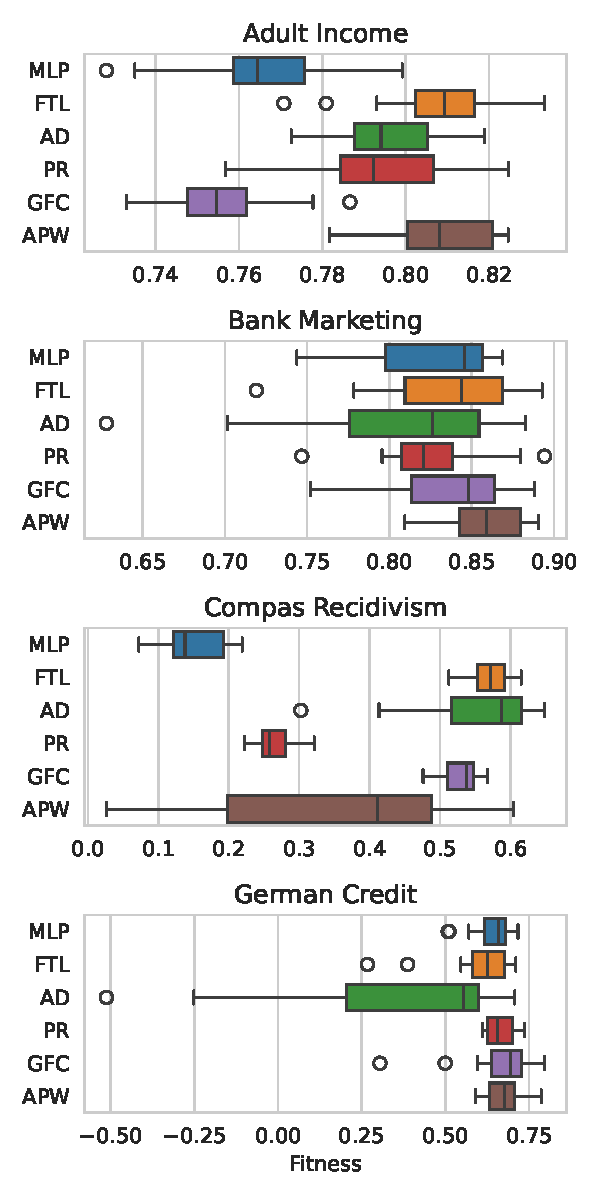
\includegraphics[width=1\linewidth]{images/boxplot_acc_odds.pdf}
\end{subfigure}
\end{figure}

Fair Transition Loss consistently demonstrates effective bias mitigation, it does so by absorbing the nuances of the dataset and the fairness metric through its transition matrices, resulting in stochastically superior fitness values in a significant number of scenarios. Additionally, the method has the capacity to effectively handle datasets with unbalanced classes when optimizing for metrics like MCC. However, it's important to recognize that Fair Transition Loss requires fine-tuning multiple hyperparameters. We thus consider that this technique is especially beneficial in setups where hyperparameter optimization is an inherent part of the prediction pipeline.

A key concern is about the potential for fairness-promoting techniques to inadvertently shift the burden onto the very group they aim to protect. This arises from the possibility that by imposing additional constraints, the method might unintentionally learn alternative ways to reproduce and even reinforce the negative social biases present in the data, thus harming the individuals it intends to safeguard.

\begin{figure}[!ht]
\centering
\caption{Results of false negatives and false positives within groups on protected promotion ($p_1$) parameter at increasing levels.}
    \label{fig:ftl_sensibility_test}
    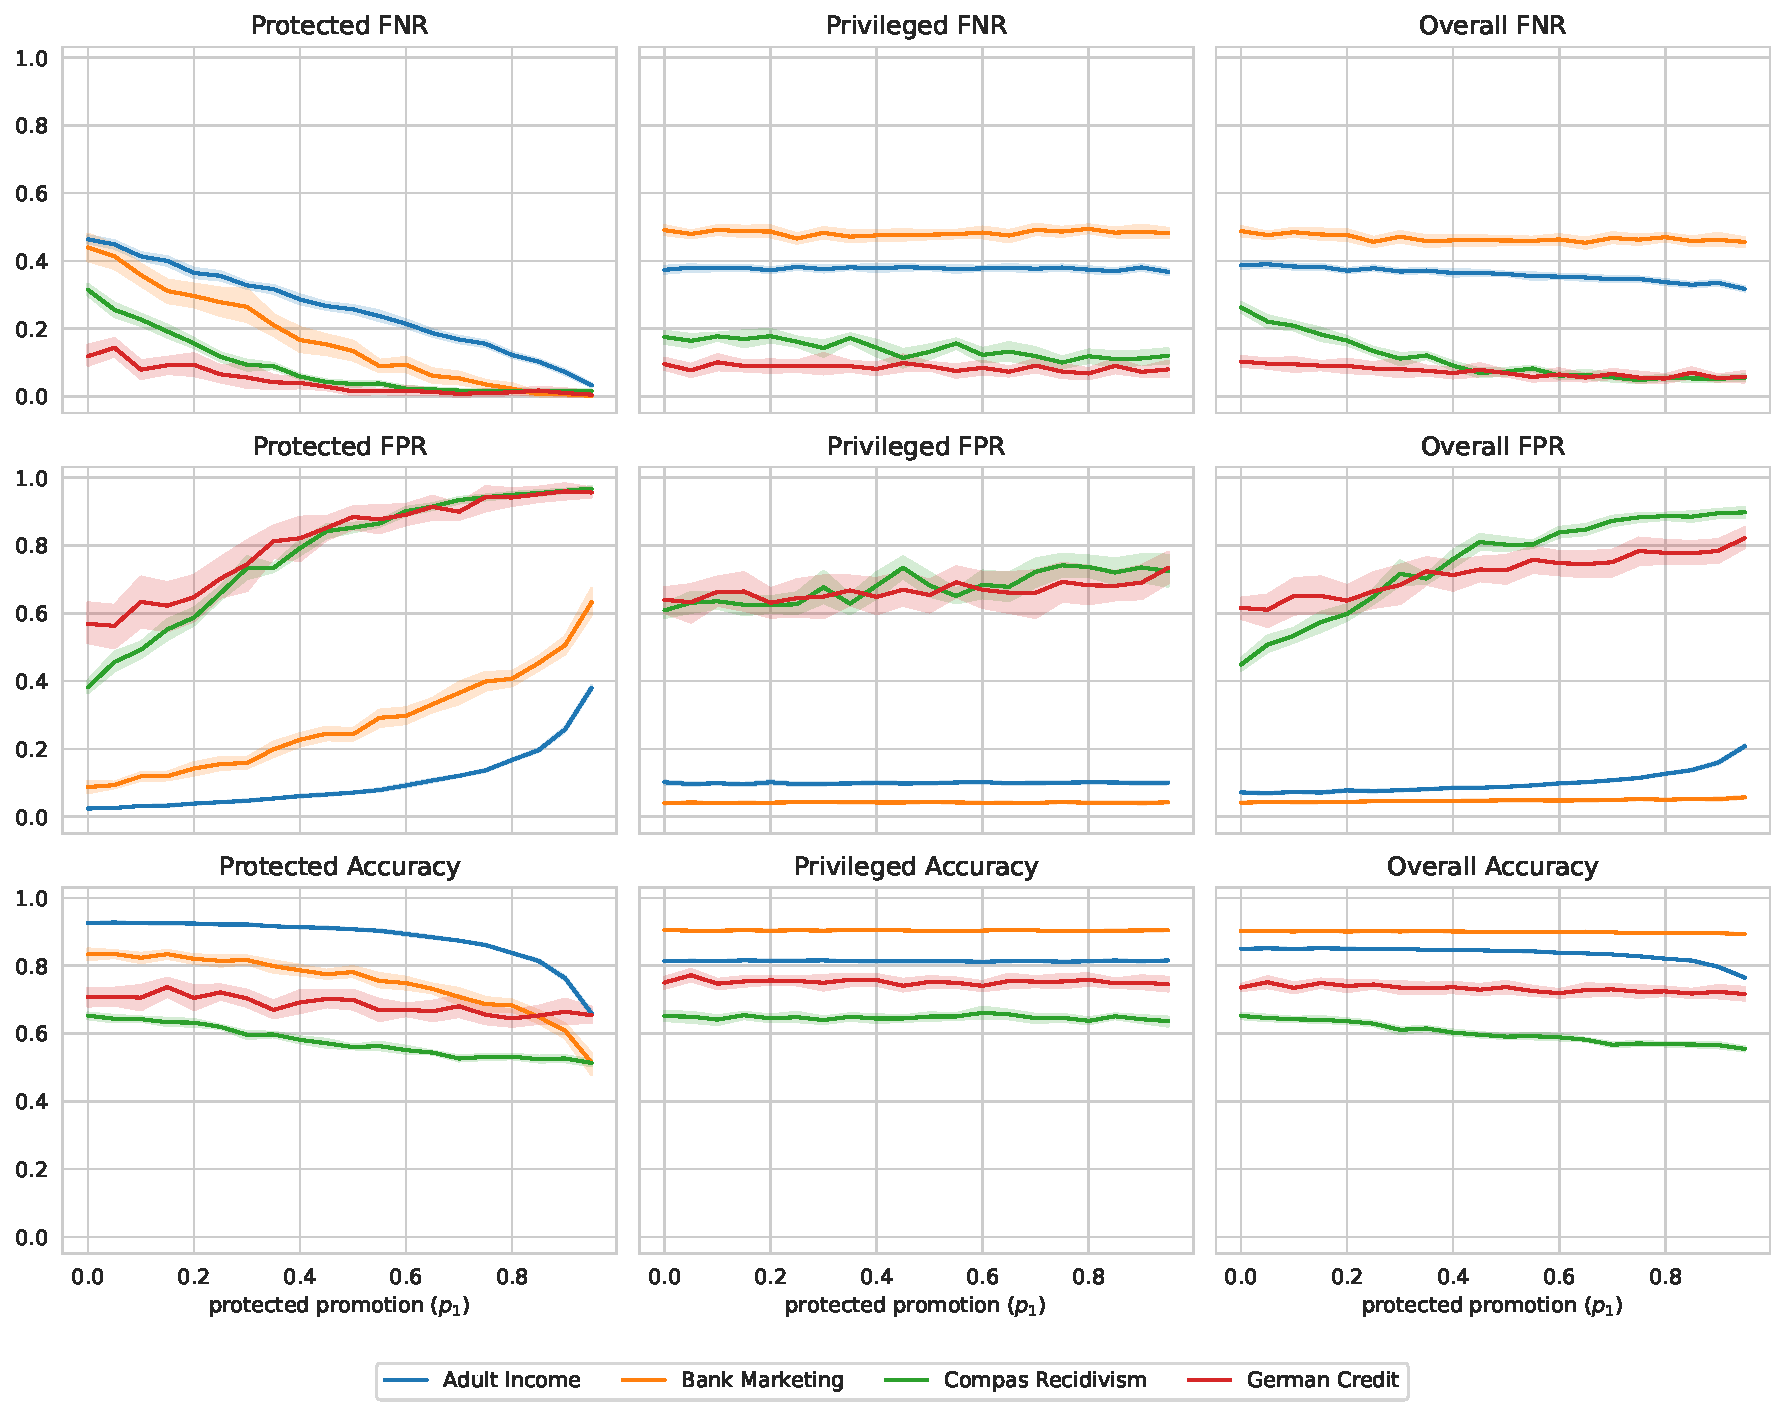
\includegraphics[width=1\linewidth]{images/ftl_sensibility_results.pdf}
\end{figure}

To evaluate the capability of FTL to address this risk, we present another experiment, where we adjusted only the protected promotion hyperparameter ($p_1$,  Equation~\ref{eq:transition_matrices}) during the FTL training, keeping all other FTL hyperparameters at zero and dropout at $0.2$. Here we follow the same re-sampling procedure, each experiment is performed over $15$ repetitions, shuffling the dataset before splitting. This experiment was conducted using the four datasets previously analyzed, and we reported the following metrics assessed over the training set: protected false negative rate, protected false positive rate, protected accuracy, privileged false negative rate, privileged false positive rate, privileged accuracy, overall false negative rate, overall false positive rate and overall accuracy.

The results, presented in Figure~\ref{fig:ftl_sensibility_test}, show that increasing the protected promotion hyperparameter value leads to a decreased false negative rate for the protected group. Meanwhile, most other monitored metrics tended towards stability to reasonable hyperparameter levels ($p_1$ under $0.95$) . An exception is the false positive rate, specially to protected group, which increased as the false negative rate decreased to keep accuracy. This pattern was consistent across all evaluated datasets. The primary aim of this experiment was to demonstrate that our proposed technique does not inadvertently penalize the protected group. Rather, the overall impact of increasing the aforementioned parameter is to effectively promote fairness for the protected group without detriment to either the privileged or protected groups. The behavior of the remaining FTL parameters is analogous, necessitating proper fine-tuning to achieve a balanced outcome. This underscores the efficacy of our method in achieving its intended purpose of reducing bias and promoting fairness in the model.

Here we present complete results with mean and standard deviation values to fitness (Equation~\ref{eq:obj_fn}), performance and fairness across multiple resampling, to a proper trade-off comparison. To each objective function and dataset methods results are ordered from higher to lower fitness mean, with corresponding standard deviation presented between parenthesis. Results corresponding each optimization scenario can be found on tables \ref{tab:complete_mcc_parity}, \ref{tab:complete_mcc_opportunity}, \ref{tab:complete_mcc_odds}, \ref{tab:complete_acc_parity}, \ref{tab:complete_acc_opportunity}, and \ref{tab:complete_acc_odds}.


\begin{table}
    \centering
    \caption{Mean and standard deviation metric values optimizing MCC and Statistical Parity in comparison with Fair Transition Loss.}\label{tab:complete_mcc_parity}
    {\footnotesize\begin{tabular}{llrrr}
    \toprule
    Dataset & Method & Fitness & MCC & Stat. Parity \\
    \midrule

    \multirow{5}{*}{\shortstack[l]{Adult\\ Income}}
& Adaptive Priority Reweighting & $0.499 (\pm0.01)$ & $0.510 (\pm0.01)$ & $0.011 (\pm0.01)$ \\
& Fair Transition Loss & $0.492 (\pm0.02)$ & $0.512 (\pm0.01)$ & $0.020 (\pm0.01)$ \\
& Prejudice Remover & $0.491 (\pm0.01)$ & $0.500 (\pm0.01)$ & $0.009 (\pm0.01)$ \\
& Adversarial Debiasing & $0.478 (\pm0.01)$ & $0.501 (\pm0.02)$ & $0.024 (\pm0.02)$ \\
& Standard MLP (baseline) & $0.395 (\pm0.01)$ & $0.581 (\pm0.01)$ & $0.185 (\pm0.01)$ \\
& Gerry Fair Classifier & $0.357 (\pm0.02)$ & $0.512 (\pm0.02)$ & $0.154 (\pm0.03)$ \\
\midrule

    \multirow{5}{*}{\shortstack[l]{Bank\\ Marketing}}
& Fair Transition Loss & $0.539 (\pm0.03)$ & $0.579 (\pm0.01)$ & $0.040 (\pm0.03)$ \\
& Adversarial Debiasing & $0.459 (\pm0.03)$ & $0.505 (\pm0.02)$ & $0.046 (\pm0.02)$ \\
& Prejudice Remover & $0.454 (\pm0.03)$ & $0.487 (\pm0.02)$ & $0.033 (\pm0.02)$ \\
& Adaptive Priority Reweighting & $0.441 (\pm0.03)$ & $0.482 (\pm0.02)$ & $0.041 (\pm0.04)$ \\
& Standard MLP (baseline) & $0.419 (\pm0.04)$ & $0.522 (\pm0.02)$ & $0.102 (\pm0.03)$ \\
& Gerry Fair Classifier & $0.358 (\pm0.04)$ & $0.428 (\pm0.02)$ & $0.070 (\pm0.03)$ \\
\midrule

    \multirow{5}{*}{\shortstack[l]{COMPAS\\ Recidivism}}
& Fair Transition Loss & $0.220 (\pm0.06)$ & $0.276 (\pm0.03)$ & $0.057 (\pm0.05)$ \\
& Adversarial Debiasing & $0.157 (\pm0.14)$ & $0.322 (\pm0.02)$ & $0.165 (\pm0.14)$ \\
& Gerry Fair Classifier & $0.141 (\pm0.04)$ & $0.289 (\pm0.06)$ & $0.148 (\pm0.06)$ \\
& Prejudice Remover & $-0.318 (\pm0.05)$ & $-0.276 (\pm0.03)$ & $0.042 (\pm0.03)$ \\
& Adaptive Priority Reweighting & $-0.412 (\pm0.35)$ & $0.194 (\pm0.07)$ & $0.606 (\pm0.29)$ \\
& Standard MLP (baseline) & $-0.511 (\pm0.05)$ & $-0.299 (\pm0.03)$ & $0.212 (\pm0.04)$ \\
\midrule

    \multirow{5}{*}{\shortstack[l]{German\\ Credit}}
& Fair Transition Loss & $0.272 (\pm0.08)$ & $0.354 (\pm0.07)$ & $0.083 (\pm0.04)$ \\
& Prejudice Remover & $0.234 (\pm0.09)$ & $0.329 (\pm0.05)$ & $0.095 (\pm0.06)$ \\
& Standard MLP (baseline) & $0.223 (\pm0.10)$ & $0.330 (\pm0.07)$ & $0.107 (\pm0.07)$ \\
& Gerry Fair Classifier & $0.221 (\pm0.09)$ & $0.291 (\pm0.11)$ & $0.071 (\pm0.06)$ \\
& Adaptive Priority Reweighting & $0.217 (\pm0.09)$ & $0.321 (\pm0.05)$ & $0.105 (\pm0.06)$ \\
& Adversarial Debiasing & $0.200 (\pm0.17)$ & $0.368 (\pm0.06)$ & $0.168 (\pm0.15)$ \\
     \bottomrule
\end{tabular}}
\end{table}

 \begin{table}
    \centering
    \caption{Mean and standard deviation metric values optimizing MCC and Equal Opportunity in comparison with Fair Transition Loss.}\label{tab:complete_mcc_opportunity}
    {\footnotesize\begin{tabular}{llrrr}
    \toprule
    Dataset & Method & Fitness & MCC & Eq. Opp. \\
    \midrule

    \multirow{5}{*}{\shortstack[l]{Adult\\ Income}}
& Fair Transition Loss & $0.523 (\pm0.02)$ & $0.576 (\pm0.02)$ & $0.052 (\pm0.02)$ \\
& Prejudice Remover & $0.509 (\pm0.05)$ & $0.558 (\pm0.02)$ & $0.049 (\pm0.03)$ \\
& Adversarial Debiasing & $0.509 (\pm0.03)$ & $0.565 (\pm0.02)$ & $0.056 (\pm0.02)$ \\
& Adaptive Priority Reweighting & $0.493 (\pm0.01)$ & $0.523 (\pm0.01)$ & $0.030 (\pm0.01)$ \\
& Standard MLP (baseline) & $0.489 (\pm0.03)$ & $0.576 (\pm0.01)$ & $0.087 (\pm0.03)$ \\
& Gerry Fair Classifier & $0.434 (\pm0.01)$ & $0.523 (\pm0.01)$ & $0.089 (\pm0.01)$ \\
\midrule

    \multirow{5}{*}{\shortstack[l]{Bank\\ Marketing}}
& Fair Transition Loss & $0.485 (\pm0.06)$ & $0.569 (\pm0.01)$ & $0.084 (\pm0.06)$ \\
& Standard MLP (baseline) & $0.439 (\pm0.03)$ & $0.514 (\pm0.02)$ & $0.075 (\pm0.03)$ \\
& Adversarial Debiasing & $0.426 (\pm0.06)$ & $0.512 (\pm0.02)$ & $0.086 (\pm0.05)$ \\
& Adaptive Priority Reweighting & $0.424 (\pm0.04)$ & $0.474 (\pm0.02)$ & $0.050 (\pm0.04)$ \\
& Prejudice Remover & $0.413 (\pm0.04)$ & $0.485 (\pm0.02)$ & $0.072 (\pm0.04)$ \\
& Gerry Fair Classifier & $0.371 (\pm0.04)$ & $0.423 (\pm0.02)$ & $0.052 (\pm0.03)$ \\
\midrule

    \multirow{5}{*}{\shortstack[l]{COMPAS\\ Recidivism}}
& Fair Transition Loss & $0.208 (\pm0.06)$ & $0.283 (\pm0.02)$ & $0.074 (\pm0.05)$ \\
& Adversarial Debiasing & $0.191 (\pm0.11)$ & $0.324 (\pm0.03)$ & $0.133 (\pm0.10)$ \\
& Gerry Fair Classifier & $0.155 (\pm0.05)$ & $0.274 (\pm0.06)$ & $0.120 (\pm0.04)$ \\
& Adaptive Priority Reweighting & $-0.111 (\pm0.18)$ & $0.260 (\pm0.04)$ & $0.371 (\pm0.17)$ \\
& Prejudice Remover & $-0.352 (\pm0.03)$ & $-0.278 (\pm0.02)$ & $0.073 (\pm0.03)$ \\
& Standard MLP (baseline) & $-0.471 (\pm0.05)$ & $-0.294 (\pm0.02)$ & $0.176 (\pm0.04)$ \\
\midrule

    \multirow{5}{*}{\shortstack[l]{German\\ Credit}}
& Adaptive Priority Reweighting & $0.299 (\pm0.08)$ & $0.373 (\pm0.06)$ & $0.075 (\pm0.05)$ \\
& Prejudice Remover & $0.283 (\pm0.10)$ & $0.391 (\pm0.07)$ & $0.107 (\pm0.06)$ \\
& Fair Transition Loss & $0.273 (\pm0.10)$ & $0.386 (\pm0.08)$ & $0.113 (\pm0.08)$ \\
& Standard MLP (baseline) & $0.270 (\pm0.07)$ & $0.352 (\pm0.05)$ & $0.082 (\pm0.04)$ \\
& Gerry Fair Classifier & $0.218 (\pm0.11)$ & $0.321 (\pm0.10)$ & $0.103 (\pm0.05)$ \\
& Adversarial Debiasing & $0.040 (\pm0.41)$ & $0.301 (\pm0.13)$ & $0.261 (\pm0.30)$ \\
     \bottomrule
\end{tabular}}
\end{table}
 \begin{table}
    \centering
    \caption{Mean and standard deviation metric values optimizing MCC and Equalized Odds in comparison with Fair Transition Loss.}\label{tab:complete_mcc_odds}
    {\footnotesize\begin{tabular}{llrrr}
    \toprule
    Dataset & Method & Fitness & MCC & Eq. Odds \\
    \midrule

    \multirow{5}{*}{\shortstack[l]{Adult\\ Income}}
& Fair Transition Loss & $0.556 (\pm0.03)$ & $0.584 (\pm0.01)$ & $0.029 (\pm0.03)$ \\
& Adaptive Priority Reweighting & $0.553 (\pm0.01)$ & $0.576 (\pm0.01)$ & $0.022 (\pm0.02)$ \\
& Prejudice Remover & $0.505 (\pm0.09)$ & $0.560 (\pm0.02)$ & $0.055 (\pm0.08)$ \\
& Adversarial Debiasing & $0.493 (\pm0.05)$ & $0.573 (\pm0.01)$ & $0.080 (\pm0.05)$ \\
& Standard MLP (baseline) & $0.489 (\pm0.03)$ & $0.580 (\pm0.01)$ & $0.091 (\pm0.03)$ \\
& Gerry Fair Classifier & $0.394 (\pm0.03)$ & $0.515 (\pm0.02)$ & $0.121 (\pm0.02)$ \\
\midrule

    \multirow{5}{*}{\shortstack[l]{Bank\\ Marketing}}
& Fair Transition Loss & $0.467 (\pm0.11)$ & $0.560 (\pm0.03)$ & $0.093 (\pm0.10)$ \\
& Adaptive Priority Reweighting & $0.441 (\pm0.06)$ & $0.500 (\pm0.01)$ & $0.059 (\pm0.06)$ \\
& Standard MLP (baseline) & $0.432 (\pm0.06)$ & $0.520 (\pm0.02)$ & $0.087 (\pm0.06)$ \\
& Prejudice Remover & $0.392 (\pm0.09)$ & $0.490 (\pm0.02)$ & $0.098 (\pm0.08)$ \\
& Adversarial Debiasing & $0.373 (\pm0.09)$ & $0.508 (\pm0.02)$ & $0.136 (\pm0.09)$ \\
& Gerry Fair Classifier & $0.344 (\pm0.07)$ & $0.422 (\pm0.02)$ & $0.078 (\pm0.06)$ \\
\midrule

    \multirow{5}{*}{\shortstack[l]{COMPAS\\ Recidivism}}
& Adaptive Priority Reweighting & $0.292 (\pm0.03)$ & $0.319 (\pm0.02)$ & $0.027 (\pm0.02)$ \\
& Adversarial Debiasing & $0.258 (\pm0.05)$ & $0.329 (\pm0.03)$ & $0.070 (\pm0.05)$ \\
& Fair Transition Loss & $0.213 (\pm0.06)$ & $0.264 (\pm0.06)$ & $0.050 (\pm0.03)$ \\
& Gerry Fair Classifier & $0.201 (\pm0.05)$ & $0.290 (\pm0.04)$ & $0.089 (\pm0.05)$ \\
& Prejudice Remover & $-0.319 (\pm0.03)$ & $-0.289 (\pm0.03)$ & $0.030 (\pm0.02)$ \\
& Standard MLP (baseline) & $-0.435 (\pm0.03)$ & $-0.292 (\pm0.02)$ & $0.143 (\pm0.03)$ \\
\midrule

    \multirow{5}{*}{\shortstack[l]{German\\ Credit}}
& Standard MLP (baseline) & $0.295 (\pm0.09)$ & $0.354 (\pm0.08)$ & $0.060 (\pm0.04)$ \\
& Fair Transition Loss & $0.274 (\pm0.10)$ & $0.361 (\pm0.08)$ & $0.087 (\pm0.05)$ \\
& Gerry Fair Classifier & $0.273 (\pm0.10)$ & $0.361 (\pm0.06)$ & $0.087 (\pm0.06)$ \\
& Prejudice Remover & $0.271 (\pm0.07)$ & $0.324 (\pm0.06)$ & $0.054 (\pm0.04)$ \\
& Adaptive Priority Reweighting & $0.261 (\pm0.08)$ & $0.326 (\pm0.06)$ & $0.065 (\pm0.05)$ \\
& Adversarial Debiasing & $0.116 (\pm0.40)$ & $0.311 (\pm0.14)$ & $0.195 (\pm0.28)$ \\
     \bottomrule
\end{tabular}}
\end{table}

 \begin{table}
    \centering
    \caption{Mean and standard deviation metric values optimizing Accuracy and Statistical Parity in comparison with Fair Transition Loss.}\label{tab:complete_acc_parity}
   {\footnotesize \begin{tabular}{llrrr}
    \toprule
    Dataset & Method & Fitness & Accuracy & Stat. Parity \\
    \midrule

    \multirow{5}{*}{\shortstack[l]{Adult\\ Income}}
& Fair Transition Loss & $0.814 (\pm0.01)$ & $0.828 (\pm0.01)$ & $0.014 (\pm0.01)$ \\
& Adaptive Priority Reweighting & $0.811 (\pm0.01)$ & $0.822 (\pm0.01)$ & $0.011 (\pm0.01)$ \\
& Adversarial Debiasing & $0.808 (\pm0.01)$ & $0.830 (\pm0.01)$ & $0.022 (\pm0.01)$ \\
& Prejudice Remover & $0.807 (\pm0.01)$ & $0.825 (\pm0.00)$ & $0.018 (\pm0.01)$ \\
& Standard MLP (baseline) & $0.666 (\pm0.01)$ & $0.851 (\pm0.00)$ & $0.184 (\pm0.01)$ \\
& Gerry Fair Classifier & $0.651 (\pm0.21)$ & $0.721 (\pm0.07)$ & $0.070 (\pm0.14)$ \\
\midrule

    \multirow{5}{*}{\shortstack[l]{Bank\\ Marketing}}
& Adversarial Debiasing & $0.869 (\pm0.03)$ & $0.901 (\pm0.00)$ & $0.031 (\pm0.02)$ \\
& Prejudice Remover & $0.860 (\pm0.02)$ & $0.898 (\pm0.00)$ & $0.038 (\pm0.02)$ \\
& Fair Transition Loss & $0.854 (\pm0.05)$ & $0.889 (\pm0.01)$ & $0.035 (\pm0.05)$ \\
& Adaptive Priority Reweighting & $0.851 (\pm0.06)$ & $0.900 (\pm0.00)$ & $0.049 (\pm0.06)$ \\
& Gerry Fair Classifier & $0.824 (\pm0.02)$ & $0.895 (\pm0.00)$ & $0.071 (\pm0.02)$ \\
& Standard MLP (baseline) & $0.799 (\pm0.04)$ & $0.902 (\pm0.00)$ & $0.103 (\pm0.03)$ \\
\midrule

    \multirow{5}{*}{\shortstack[l]{COMPAS\\ Recidivism}}
& Adversarial Debiasing & $0.538 (\pm0.07)$ & $0.670 (\pm0.02)$ & $0.132 (\pm0.08)$ \\
& Fair Transition Loss & $0.501 (\pm0.15)$ & $0.600 (\pm0.05)$ & $0.099 (\pm0.14)$ \\
& Gerry Fair Classifier & $0.501 (\pm0.05)$ & $0.614 (\pm0.05)$ & $0.113 (\pm0.07)$ \\
& Prejudice Remover & $0.308 (\pm0.03)$ & $0.359 (\pm0.01)$ & $0.052 (\pm0.02)$ \\
& Standard MLP (baseline) & $0.146 (\pm0.03)$ & $0.354 (\pm0.02)$ & $0.208 (\pm0.02)$ \\
& Adaptive Priority Reweighting & $-0.105 (\pm0.26)$ & $0.584 (\pm0.03)$ & $0.689 (\pm0.23)$ \\
\midrule

    \multirow{5}{*}{\shortstack[l]{German\\ Credit}}
& Prejudice Remover & $0.684 (\pm0.05)$ & $0.757 (\pm0.02)$ & $0.073 (\pm0.06)$ \\
& Standard MLP (baseline) & $0.639 (\pm0.06)$ & $0.752 (\pm0.02)$ & $0.113 (\pm0.06)$ \\
& Gerry Fair Classifier & $0.621 (\pm0.09)$ & $0.712 (\pm0.12)$ & $0.090 (\pm0.04)$ \\
& Fair Transition Loss & $0.616 (\pm0.20)$ & $0.715 (\pm0.06)$ & $0.098 (\pm0.17)$ \\
& Adaptive Priority Reweighting & $0.589 (\pm0.08)$ & $0.682 (\pm0.03)$ & $0.093 (\pm0.08)$ \\
& Adversarial Debiasing & $0.430 (\pm0.33)$ & $0.713 (\pm0.09)$ & $0.283 (\pm0.26)$ \\
     \bottomrule
\end{tabular}}
\end{table}


\begin{table}
    \centering
    \caption{Mean and standard deviation metric values optimizing Accuracy and Equal Opportunity in comparison with Fair Transition Loss.}\label{tab:complete_acc_opportunity}
    {\footnotesize \begin{tabular}{llrrr}
    \toprule
    Dataset & Method & Fitness & Accuracy & Eq. Opp. \\
    \midrule

    \multirow{5}{*}{\shortstack[l]{Adult\\ Income}}
& Adaptive Priority Reweighting & $0.808 (\pm0.01)$ & $0.837 (\pm0.00)$ & $0.029 (\pm0.01)$ \\
& Fair Transition Loss & $0.808 (\pm0.02)$ & $0.842 (\pm0.01)$ & $0.034 (\pm0.02)$ \\
& Adversarial Debiasing & $0.796 (\pm0.01)$ & $0.849 (\pm0.00)$ & $0.052 (\pm0.01)$ \\
& Prejudice Remover & $0.794 (\pm0.02)$ & $0.845 (\pm0.01)$ & $0.051 (\pm0.01)$ \\
& Standard MLP (baseline) & $0.765 (\pm0.02)$ & $0.850 (\pm0.00)$ & $0.084 (\pm0.02)$ \\
& Gerry Fair Classifier & $0.756 (\pm0.01)$ & $0.788 (\pm0.03)$ & $0.032 (\pm0.04)$ \\
\midrule

    \multirow{5}{*}{\shortstack[l]{Bank\\ Marketing}}
& Adaptive Priority Reweighting & $0.858 (\pm0.02)$ & $0.897 (\pm0.00)$ & $0.039 (\pm0.03)$ \\
& Gerry Fair Classifier & $0.837 (\pm0.04)$ & $0.895 (\pm0.00)$ & $0.058 (\pm0.04)$ \\
& Fair Transition Loss & $0.833 (\pm0.05)$ & $0.892 (\pm0.01)$ & $0.059 (\pm0.05)$ \\
& Prejudice Remover & $0.827 (\pm0.04)$ & $0.898 (\pm0.00)$ & $0.071 (\pm0.04)$ \\
& Standard MLP (baseline) & $0.826 (\pm0.04)$ & $0.901 (\pm0.00)$ & $0.075 (\pm0.04)$ \\
& Adversarial Debiasing & $0.807 (\pm0.07)$ & $0.902 (\pm0.00)$ & $0.095 (\pm0.07)$ \\
\midrule

    \multirow{5}{*}{\shortstack[l]{COMPAS\\ Recidivism}}
& Fair Transition Loss & $0.572 (\pm0.03)$ & $0.631 (\pm0.04)$ & $0.059 (\pm0.03)$ \\
& Adversarial Debiasing & $0.553 (\pm0.09)$ & $0.669 (\pm0.01)$ & $0.116 (\pm0.09)$ \\
& Gerry Fair Classifier & $0.530 (\pm0.03)$ & $0.637 (\pm0.04)$ & $0.107 (\pm0.05)$ \\
& Adaptive Priority Reweighting & $0.356 (\pm0.18)$ & $0.643 (\pm0.02)$ & $0.287 (\pm0.18)$ \\
& Prejudice Remover & $0.264 (\pm0.03)$ & $0.357 (\pm0.01)$ & $0.093 (\pm0.02)$ \\
& Standard MLP (baseline) & $0.155 (\pm0.04)$ & $0.350 (\pm0.02)$ & $0.195 (\pm0.04)$ \\
\midrule

    \multirow{5}{*}{\shortstack[l]{German\\ Credit}}
& Adaptive Priority Reweighting & $0.674 (\pm0.06)$ & $0.750 (\pm0.03)$ & $0.076 (\pm0.04)$ \\
& Prejudice Remover & $0.664 (\pm0.05)$ & $0.748 (\pm0.02)$ & $0.084 (\pm0.04)$ \\
& Gerry Fair Classifier & $0.662 (\pm0.12)$ & $0.719 (\pm0.12)$ & $0.057 (\pm0.07)$ \\
& Standard MLP (baseline) & $0.638 (\pm0.06)$ & $0.738 (\pm0.04)$ & $0.101 (\pm0.05)$ \\
& Fair Transition Loss & $0.599 (\pm0.12)$ & $0.711 (\pm0.05)$ & $0.112 (\pm0.11)$ \\
& Adversarial Debiasing & $0.368 (\pm0.38)$ & $0.685 (\pm0.10)$ & $0.317 (\pm0.30)$ \\
     \bottomrule
\end{tabular} }
\end{table}

 \begin{table}
    \centering
    \caption{Mean and standard deviation metric values optimizing Accuracy and Equalized Odds in comparison with Fair Transition Loss.}\label{tab:complete_acc_odds}
    {\footnotesize \begin{tabular}{llrrr}
    \toprule
    Dataset & Method & Fitness & Accuracy & Eq. Odds \\
    \midrule

    \multirow{5}{*}{\shortstack[l]{Adult\\ Income}}
& Adaptive Priority Reweighting & $0.829 (\pm0.01)$ & $0.847 (\pm0.00)$ & $0.018 (\pm0.01)$ \\
 & Prejudice Remover & $0.810 (\pm0.02)$ & $0.846 (\pm0.00)$ & $0.036 (\pm0.02)$ \\
 & Fair Transition Loss & $0.787 (\pm0.08)$ & $0.826 (\pm0.07)$ & $0.039 (\pm0.04)$ \\
 & Adversarial Debiasing & $0.756 (\pm0.03)$ & $0.848 (\pm0.00)$ & $0.092 (\pm0.03)$ \\
 & Standard MLP (baseline) & $0.752 (\pm0.04)$ & $0.849 (\pm0.00)$ & $0.097 (\pm0.04)$ \\
 & Gerry Fair Classifier & $0.705 (\pm0.07)$ & $0.751 (\pm0.09)$ & $0.046 (\pm0.05)$ \\
\midrule

    \multirow{5}{*}{\shortstack[l]{Bank\\ Marketing}}
& Adaptive Priority Reweighting & $0.846 (\pm0.05)$ & $0.901 (\pm0.00)$ & $0.055 (\pm0.05)$ \\
& Gerry Fair Classifier & $0.837 (\pm0.06)$ & $0.893 (\pm0.00)$ & $0.057 (\pm0.06)$ \\
& Standard MLP (baseline) & $0.800 (\pm0.06)$ & $0.902 (\pm0.00)$ & $0.102 (\pm0.06)$ \\
& Fair Transition Loss & $0.799 (\pm0.10)$ & $0.891 (\pm0.01)$ & $0.092 (\pm0.10)$ \\
& Prejudice Remover & $0.781 (\pm0.07)$ & $0.899 (\pm0.00)$ & $0.118 (\pm0.07)$ \\
& Adversarial Debiasing & $0.750 (\pm0.09)$ & $0.900 (\pm0.00)$ & $0.150 (\pm0.09)$ \\
\midrule

    \multirow{5}{*}{\shortstack[l]{COMPAS\\ Recidivism}}
& Adaptive Priority Reweighting & $0.642 (\pm0.03)$ & $0.669 (\pm0.01)$ & $0.027 (\pm0.02)$ \\
& Fair Transition Loss & $0.594 (\pm0.04)$ & $0.648 (\pm0.01)$ & $0.054 (\pm0.03)$ \\
& Adversarial Debiasing & $0.594 (\pm0.07)$ & $0.672 (\pm0.02)$ & $0.078 (\pm0.06)$ \\
& Gerry Fair Classifier & $0.558 (\pm0.05)$ & $0.647 (\pm0.02)$ & $0.088 (\pm0.04)$ \\
& Prejudice Remover & $0.287 (\pm0.03)$ & $0.342 (\pm0.01)$ & $0.055 (\pm0.03)$ \\
& Standard MLP (baseline) & $0.218 (\pm0.05)$ & $0.353 (\pm0.01)$ & $0.135 (\pm0.05)$ \\
\midrule

    \multirow{5}{*}{\shortstack[l]{German\\ Credit}}
& Adaptive Priority Reweighting & $0.716 (\pm0.04)$ & $0.750 (\pm0.02)$ & $0.034 (\pm0.03)$ \\
& Standard MLP (baseline) & $0.681 (\pm0.08)$ & $0.747 (\pm0.03)$ & $0.066 (\pm0.06)$ \\
& Prejudice Remover & $0.648 (\pm0.06)$ & $0.743 (\pm0.03)$ & $0.095 (\pm0.06)$ \\
& Gerry Fair Classifier & $0.643 (\pm0.13)$ & $0.707 (\pm0.13)$ & $0.063 (\pm0.04)$ \\
& Fair Transition Loss & $0.622 (\pm0.26)$ & $0.705 (\pm0.10)$ & $0.083 (\pm0.17)$ \\
& Adversarial Debiasing & $0.530 (\pm0.33)$ & $0.713 (\pm0.10)$ & $0.183 (\pm0.24)$ \\
     \bottomrule
\end{tabular}}
\end{table}
  \chapter{Correlation based penalty function}\label{chap:rpr}

In this chapter, we propose a novel regularization factor to penalize the use of features highly correlated with a protected attribute by a machine learning model, aiming to avoid the redlining effect~\citep{Pedreschi2008}. The proposed penalization factor is applied directly to the input weights of a Multi-Layer Perceptron, using a strategy that proportionately penalizes features use based on their correlation with the sensitive feature.

\section{Preliminaries} \label{sec:rpr_preliminaries}

The phenomena known as redlining effect~\citep{Pedreschi2008} consists in the unintended use of proxy variables to the sensitive feature by the model, which can lead model to produce indirect discrimination in their outcomes.  Thus, the insight here is to penalize the use of those proxy features by the model proportionally according its correlation with sensitive feature in order to avoid redlining effed. The proposed regularization approach uses the recently described Chatterjee's xi correlation coefficient~\cite{chatterjee2020new}, which robustly asses whether a random variable can be described as a function of another one, as a measure of the potential of given feature to be used by the model as a proxy to the sensitive feature. 

Before discussing this approach, we start defining some common correlation coefficients and providing a proper comparison within Chatterjee's correlation. For purpose of simplicity we describe only the most commonly used form, more complex formulations involving additional terms depending on available data should be considered to most of coefficients. Also, we present some related approaches, specially those ones that, like ours, use regularization and penalty factors to avoid indirect discrimination.

The Pearson correlation coefficient, denoted by $\rho$ and defined in Definition~\ref{def:pearson}, is a measure of the linear relationship between two random variables. The Pearson correlation coefficient ranges from $-1$ to $1$, where $1$ indicates a perfect positive linear relationship, $-1$ indicates a perfect negative linear relationship, and $0$ indicates no linear relationship.

\begin{definition}[Pearson correlation coefficient]\label{def:pearson}
Let  $X$ and $Y$\ random variables. The Pearson correlation coefficient $\rho$ between $X$ and $Y$ can be defined as  
\begin{equation}
\rho = \frac{\mathrm{Cov}(X, Y)}{\sigma_X \sigma_Y},
\end{equation}
where $\mathrm{Cov}(X, Y)$ is the covariance between $X$ and $Y$, while $\sigma_X$ and $\sigma_Y$ the standard deviations of $X$ and $Y$, respectively. 
\end{definition}

Spearman's rank correlation coefficient, denoted by $\rho_s$ and defined in Definition~\ref{def:spearman}, measures the strength and direction of the monotonic relationship between two ranked (ordered) variables.  As like Pearson correlation coefficient, Spearman's rank correlation coefficient ranges from $-1$ to $1$, where $1$ indicates a perfect positive relationship, $-1$ indicates a perfect negative relationship, and $0$ indicates no relationship.
 
\begin{definition}[Spearman's correlation coefficient]\label{def:spearman}
Let $X$ and $Y$\ random variables, $n$ the sample size and $X_i, \, Y_i$ the $i$-th observations to $i = 1 \ldots n$. Let $R_{X_i}, \, R_{Y_i}$ the rank of observations $X_i, \, Y_i$, i.e. the position of $X_i, \, Y_i$ by ordering the samples, respectively. The Spearman's rank correlation coefficient  $\rho_s$ between $X$ and $Y$ can be defined to non-repeated observation values as 
\begin{equation}\label{eq:spearman}
\rho_s = 1 - \frac{6 \sum\limits_{i=1}^{n}d_i^2}{n(n^2 - 1)},
\end{equation}
where $d_i = R_{X_i} - R_{Y_i}$.
\end{definition}

Kendall's rank correlation coefficient, denoted by $\tau$ and defined in Definition~\ref{def:kendall},  indicates the strength and direction of association between two variables. It is based on the relative ordering of pairs of observations rather than their actual values. Here we interpret the correlation values as like in Spearman's and Pearson's correlation coefficients, ranging from $-1$ to $1$, where $1$ indicates a perfect positive relationship, $-1$ a perfect negative relationship, and $0$  no linear relationship.

\begin{definition}[Kendall's correlation coefficient]\label{def:kendall}
Let two variables $X$ and $Y$ sampled with $n$ pairs of observations $(X_i, Y_i)$ for $i = 1, 2, \ldots, n$. A pair of observations $(X_i, Y_i)$ and $(X_j, Y_j)$ is \textbf{concordant} if the ranks (order) of both elements agree, i.e., to $i < j$ either $X_i > X_j$ and $Y_i > Y_j)$ or $X_i < X_j$ and $Y_i < Y_j$. Otherwise their are considered \textbf{discordant}, i.e., either $X_i > X_j$ and $Y_i < Y_j$ or $X_i < X_j$ and $Y_i > Y_j$. The Kendall's rank correlation coefficient $\tau$ between $X$ and $Y$ can be defined as 
\begin{equation}\label{eq:kendall}
\tau = \frac{2(N_c - N_d)}{n(n-1)},
\end{equation}
where $N_c$ is the number of concordant observation and $N_d$ the number of discordant observations.
\end{definition}

Chatterjee's rank correlation coefficient, denoted by $\xi$ and defined in Definition~\ref{def:chatterjee}, is designed to robustly measure the degree of dependence between two variables without assuming any specific type of relationship and capturing noise nuances.  The previously described correlation coefficients are not effective on detecting associations that are not monotonic, even in complete absence of noise.

This correlation coefficient asses whether a random variable can be described as a function of another one. Differently from correlation coefficients described before, this coefficient ranges from 0 to 1, where 0 indicates independence and 1 indicates a perfect functional relationship. Also this correlation is not symmetric, i.e., the correlation between $X$ and $Y$ may differ from between $Y$ and $X$. 

\begin{definition}[Chatterjee's correlation coefficient]\label{def:chatterjee}
Let two variables $X$ and $Y$ , where $Y$ is not a constant, sampled with $n$ pairs of observations $(X_i, Y_i)$ for $i = 1, 2, \ldots, n$. The Chatterjee's rank correlation coefficient $\tau$ between $X$ and $Y$ when there are no ties among $Y$ can be defined as 
\begin{equation}\label{eq:chatterjee}
\xi = 1 - \frac{3 \sum\limits_{i=1}^{n-1} |R_{i+1} - R_i|}{n^2 - 1},
\end{equation}
where $R_i$ is the rank of $Y_i$ in the ordered sequence of $Y$ values corresponding to the sorted $X$ values. 
\end{definition}

To illustrate some characteristics of Chatterjee's rank correlation coefficient we compare those results on Anscombe's quartet~\citep{anscombe1973} along with Pearson's, Spearman's and Kendall's correlation coefficients. The Anscombe's quartet (Table~\ref{tab:anscombe}) is a set of four different datasets that have nearly identical simple descriptive statistics, yet very different distribution, which is clear on Figure~\ref{fig:anscombe}. As an additional resource, a line representing a linear regression over the data is plotted within the points, enforcing that they present nearly identical simple descriptive statistics.

\begin{table}[ht]
\centering
\caption{Anscombe's quartet}
\label{tab:anscombe}
\begin{tabular}{rr|rr|rr|rr}
\toprule
\multicolumn{2}{c|}{I} & \multicolumn{2}{c|}{II} & \multicolumn{2}{c|}{III} & \multicolumn{2}{c}{IV} \\

\multicolumn{1}{c}{$x$} & \multicolumn{1}{c|}{$y$} & \multicolumn{1}{c}{$x$} & \multicolumn{1}{c|}{$y$} & \multicolumn{1}{c}{$x$} & \multicolumn{1}{c|}{$y$} & \multicolumn{1}{c}{$x$} & \multicolumn{1}{c}{$y$} \\
\midrule
10.0 & 8.04 & 10.0 & 9.14 & 10.0 & 7.46 & 8.0 & 6.58 \\
8.0 & 6.95 & 8.0 & 8.14 & 8.0 & 6.77 & 8.0 & 5.76 \\
13.0 & 7.58 & 13.0 & 8.74 & 13.0 & 12.74 & 8.0 & 7.71 \\
9.0 & 8.81 & 9.0 & 8.77 & 9.0 & 7.11 & 8.0 & 8.84 \\
11.0 & 8.33 & 11.0 & 9.26 & 11.0 & 7.81 & 8.0 & 8.47 \\
14.0 & 9.96 & 14.0 & 8.10 & 14.0 & 8.84 & 8.0 & 7.04 \\
6.0 & 7.24 & 6.0 & 6.13 & 6.0 & 6.08 & 8.0 & 5.25 \\
4.0 & 4.26 & 4.0 & 3.10 & 4.0 & 5.39 & 19.0 & 12.50 \\
12.0 & 10.84 & 12.0 & 9.13 & 12.0 & 8.15 & 8.0 & 5.56 \\
7.0 & 4.82 & 7.0 & 7.26 & 7.0 & 6.42 & 8.0 & 7.91 \\
5.0 & 5.68 & 5.0 & 4.74 & 5.0 & 5.73 & 8.0 & 6.89 \\
\bottomrule
\end{tabular}
\end{table}

Comparing correlation coefficients, it is evident that Pearson's $\rho$ does not properly capture the peculiarities of Anscombe's quartet. Although the four datasets present the same correlation coefficient, they exhibit very different distribution. Spearman's $\rho_s$ and Kendall's $\tau$ performs very similarly each other, properly capturing relevant characteristics, albeit Kendall's $\tau$ demonstrates to be more exigent on assigning high correlation values. Chatterjee's $\xi$ is even more exigent, pursuing the behavior of capturing functional relations between data, considering noise. For example, the first quartet presents a small $\xi$ as it contains relevant noise, despite the points are effectively linearly disposed. Albeit the second quartet demonstrate a non linear distribution, the data has lower noise influence, presenting a more functional relationship. Thus, to Chatterjee's correlation the second presents a higher coefficient than the first, which is not equivalently captured by Spearman's and Kendall's. 
\begin{figure}[!ht]
\centering
\caption{Multiple correlation coefficients on Anscombe's quartet.}\label{fig:anscombe}
    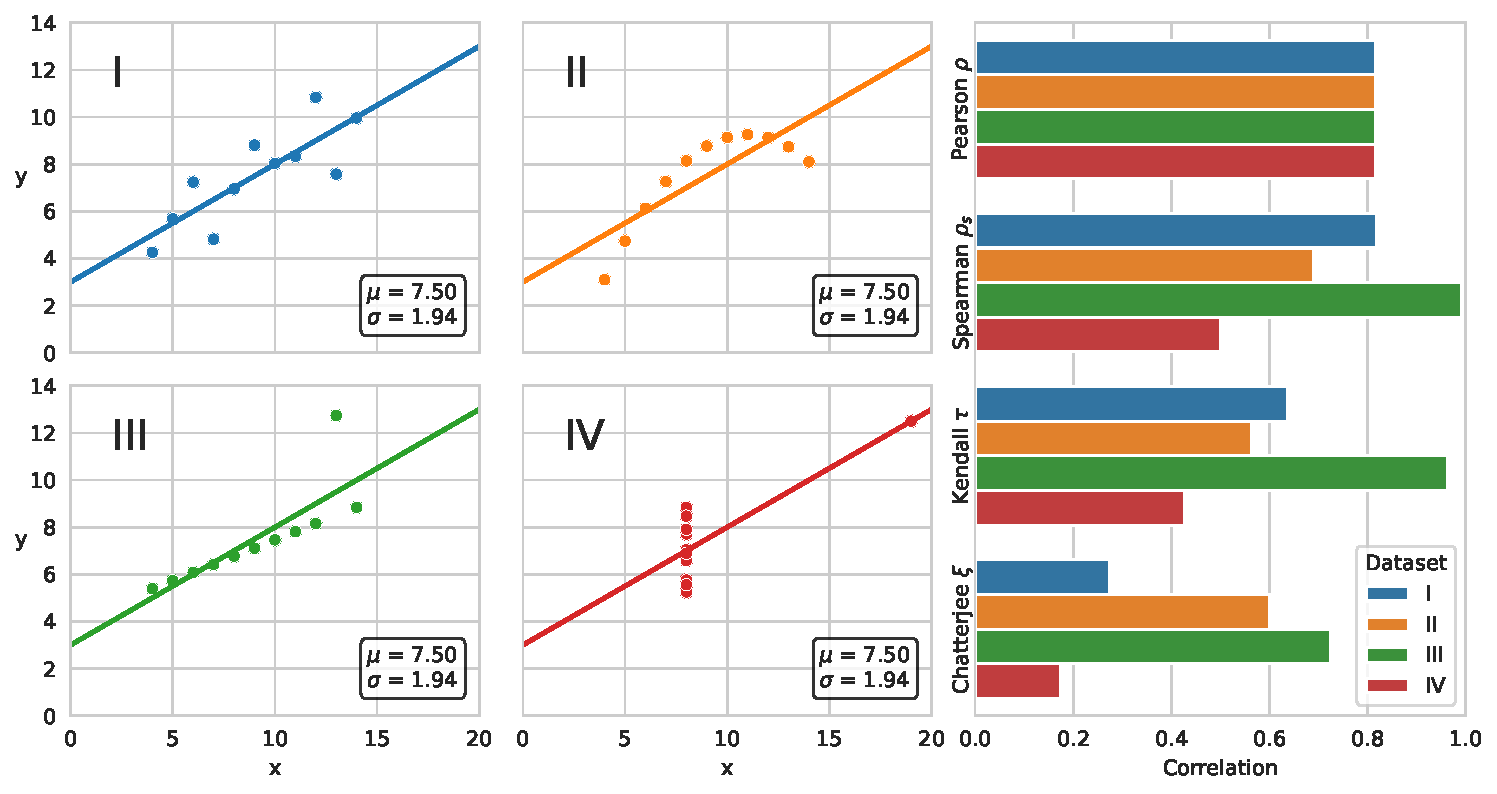
\includegraphics[width=1\linewidth]{images/anscombe_quartet.pdf}
\end{figure}



As a resource to defining the proposed redlining penalty method we describe the L2 regularization. This regularization term, a.k.a. weight decay, is a common technique used to prevent overfitting in machine learning models, including the Multi-Layer Perceptron (MLP). The L2 regularization adds a penalty term to the loss function that is proportional to the sum of the squares of the model parameters (weights). This encourages the model to keep the weights small, which can help improving generalization.

Let $\mathbf{W}^{(l)}$ represent the weight matrix for the $l$-th layer of the MLP, and let $\mathbf{b}^{(l)}$ denote the corresponding bias vector. The primary loss function of the network, $L_0$, could be any suitable loss function such as the mean squared error for regression or the cross-entropy loss for classification. The L2 regularization term for a single layer is given by
\begin{equation}
R(\mathbf{W}^{(l)}) = \frac{1}{2} \sum_{i=1}^{d_l} \sum_{j=1}^{h_l} \left( W^{(l)}_{ij} \right)^2,
\end{equation}
where $d_l$ and $h_l$ are the dimensions of the weight matrix $\mathbf{W}^{(l)}$, and $W^{(l)}_{ij}$ is the weight connecting the $i$-th input neuron to the $j$-th neuron in the $l$-th layer. Thus, the total regularization term for the entire network, considering all layers, is
\begin{equation}
R(\mathbf{W}) = \frac{1}{2} \sum_{l=1}^{L} \sum_{i=1}^{d_l} \sum_{j=1}^{h_l} \left( W^{(l)}_{ij} \right)^2,
\end{equation}
where $L$ is the total number of layers in the network. Furthermore, the total loss function $L$ for the MLP, incorporating the L2 regularization term, is defined as
\begin{equation}
L = L_0 + \lambda \; R(\mathbf{W}),
\end{equation}
where $\lambda$ is a scalar hyperparameter that controls the overall strength of the regularization.

By adding this regularization term, the optimization process aims to minimize the primary loss $L_0$ along with keeping the weights small, thereby helping to reduce the model complexity and prevent overfitting. The gradient descent updates for the weights will be adjusted to account for the regularization term, effectively shrinking the weights during the training process.

Although many fair machine learning techniques are based on imposing constraints to achieve reasonable values under specific fairness definitions and metrics~\citep{Mehrabi2019,caton2023,Hort2023}, the approach of integrating these constraints as regularization factors remains underexplored. One foundational fairness technique, the Prejudice Remover Regularizer~\citep{Kamishima2012}, accomplishes this objective by measuring and penalizing indirect prejudice through a \textit{prejudice index} alongside an L2 regularization.

Relevant regularization approaches to fair machine learning include the dual form for Fairness Constraints through Decision Boundary Covariance by \cite{Zafar2017b} and the example-based and model-agnostic Paired-Consistency approach~\citep{Horesh2020}. A notable approach proposed by \cite{Baharlouei2020} includes a general min-max framework for fair inference using the Rényi correlation coefficient~\citep{Renyi1959} as a regularization term. Additional recent developments in this research area can be found in the works of \cite{Olfat2020}, \cite{Yu2022}, and \cite{jung2023}.

\section{Redlining Penalty Regularizer} \label{sec:rpr_proposal}

Here we propose the Redlining Penalty Regularizer (RPR), a novel regularization term that penalizes the weights of features highly correlated with the sensitive attribute in order to prevent the redlining effect. By incorporating this penalty into the loss function of the neural network, the model is encouraged to reduce its reliance on sensitive attributes and their proxies, thus promoting fairer predictions. To the best of our knowledge, this the first approach to incorporate a regularization term that proportionately penalizes the features weights on the input layer according its correlation to sensitive attribute to prevent the redlining effect.

As referred before, the Chatterjee's Xi Correlation Coefficient distinguish from many other by providing a measure of how much one random variable can be expressed as a function of another, with a range from $0$ to $1$. This characteristics is relevant to the proposed use, to capture redlining effect, as of this phenomena happens exactly when the sensitive feature can be inferred by another one, producing the same harmful effects whether the correlation is positive or negative. Naturally it would be possible to use the absolute value of correlation coefficient such as Pearson, Spearman and Kendall, but this strategy could lead to some kind of information loss. Another relevant characteristics of this correlation coefficient is the ability to capture sophisticated non-linearities, including non-monotonic ones, and the effects of noise on variable's distribution, conditions frequently present in proxy feature relationships. 

Thus, let $X \in \mathbb{R}^{n \times d}$ be a dataset where $n$ represents the number of instances and $d$ represents the number of features. Let $X_i \in \mathbb{R}^n$ denote the $i$-th feature of the dataset, and let $A = X_i \in \mathbb{R}^n$ be a sensitive (protected) feature for some $i$. In this neural network, $\mathbf{W}^{(1)} \in \mathbb{R}^{d \times h}$ is the weight matrix for the first hidden layer, with $h$ being the number of neurons in this layer. Additionally, $\lambda$ is a scalar that controls the overall strength of the regularization.

Thus, the proposed regularization term $R(\mathbf{W}^{(1)})$ applied to the weight matrix $\mathbf{W}^{(1)}$ only on the first hidden layer, defined as 
\begin{equation}\label{eq:xi_reg}
R(\mathbf{W}^{(1)}) = \sum_{i=1}^d \xi_n(X_i,\,A) \sum_{j=1}^h (W^{(1)}_{ij})^2,
\end{equation}
where $W^{(1)}_{ij}$ are the weights connecting the $i$-th input feature to the $j$-th neuron in the first hidden layer. Here, the Chatterjee's Xi Correlation Coefficient $\xi_n(X_i,\,A)$ between the $i$-th input feature $X_i$ and the sensitive feature $A$ acts as the regularization strength for the $i$-th input feature. The greater $i$-th input feature dependence on sensitive feature the greater the penalization factor enforcing lower values to those weights.

Thus, the total loss function $L$ to a MLP, incorporating the sensitive-feature-specific $L_2$ regularization, is defined as
\begin{equation}\label{eq:total_regularized_loss}
L = L_0 + \lambda \; R(\mathbf{W}^{(1)}),
\end{equation}
where $L_0$ is the primary loss function of the network. This formulation ensures that the model's learning process penalizes weights with high values associated with features highly correlated to the sensitive attribute, thereby reducing the potential for biased decisions influenced by redlining effect.

This formulation differs from similar approaches to regularization in order to achieve fairness in machine learning by two fundamental points.  The first one is that here the regularization acts as a focused penalty factor through the use of the correlation of each feature to the sensitive one, reducing it's effect on less correlated features and boosting on the highly correlated ones. The second point is that this proposed penalty does not acts as a common regularizer, by imposing small values on every model's parameter. Rather, it penalizes the use of each feature according it's correlation to the sensitive one by exclusively acting on the input layer weights, that is, the usage level of each feature by hidden units.

With the combination of characteristics tailored by this formulation and the chosen correlation coefficient we do expects effectively avoiding the use of indirect sensitive feature predictors within the model, thus mitigating redlining effect.

\section{Experimental setup} \label{sec:rpr_experimental}

In this section, we detail the experimental setup employed to benchmark the proposed regularization within both Standard MLP with Cross Entropy Loss and a MLP using Fair Transition Loss. Both MLP model uses two hidden layers with $100$ hidden units each, $ReLU$ activation function, batch size of $64$, $50$ epochs early stopped at $3$ epochs without improvement~\citep{Li2020} and softmax in output, trained with ADAM optimizer~\citep{KingmaB14} and learning rate at $3\mathrm{e}{-4}$. 

The overall experimental methodology follows same principles of those used on Fair Transition Loss evaluation. There are two phases: hyperparameter tuning and testing. In the hyperparameter tuning phase we perform a Bandit-Based pruning approach using HyperBand~\citep{Li2018} with Tree-structured Parzen Estimator Sampler (TPE)~\citep{bergstra2011} over $100$ trials. At each trial a fitness function is evaluated by performing a complete training and validation, where both model performance and fairness metrics are assessed. The fitness function is computed based on the objective defined in Equation~\ref{eq:obj_fn}. 

Once the best hyperparameters are selected, we proceed to the testing phase, where a new training is conducted using those optimal hyperparameters. After this training, we evaluate the model's performance on a separate test set that was not used during the hyperparameter tuning phase, which are reported. This complete tuning-training-testing described is repeated $15$ times within random re-sampling then we proceed to comparison. Here the re-sampling consists in shuffling the whole dataset before splitting, as described before

As the objective defined in Equation~\ref{eq:obj_fn} can be achieved with different performance and fairness metrics, we compare the proposed regularization schema within Standard MLP and MLP with FTL in different optimization scenarios, considering as performance metrics Accuracy (Acc.) and Mathews Correlation Coefficient (MCC), while the fairness metrics considered are Statistical Parity (Stat. Parity), Equal Opportunity (Eq. Opp.) and Equalized Odds (Eq. Odds). Those pursued metrics lead us to the following optimization scenarios: MCC and Statistical Parity; MCC and Equal Opportunity; MCC and Equalized Odds; Accuracy and Statistical Parity; Accuracy and Equal Opportunity; Accuracy and Equalized Odds.

\begin{table}[ht]
\centering
\caption{Hyperparameters search ranges or options of each method.}\label{tab:hyperparameters_rpr}
{\footnotesize
\begin{tabular}{lll}
\toprule
Method & Parameter & Range/options \\ \midrule
 Standard MLP without regularization (baseline) & dropout & $[0.0,\,0.2]$  \vspace{1ex} \\
 Standard MLP with RPR & dropout & $[0.0,\,0.2]$  \vspace{1ex} \\
 & $\lambda$ & $\{1e^{-2}, 1^{e-3}, 1^{e-4}\}$ \\
 Fair Transition Loss without regularization & $d_0,p_0,d_1,p_1$ & $[0.0,\,1.0]$ \\
 &  dropout & $[0.0,\,0.2]$ \\
 Fair Transition Loss with RPR & $d_0,p_0,d_1,p_1$ & $[0.0,\,1.0]$ \\
 &  dropout & $[0.0,\,0.2]$ \\
 & $\lambda$ & $\{1e^{-2}, 1^{e-3}, 1^{e-4}\}$ \\
\bottomrule
\end{tabular}
}
\end{table}

Table~\ref{tab:hyperparameters_rpr} presents the methods hyperparameters along with their corresponding search ranges or options. While each method may possess a varying number of hyperparameters and range sizes, all are optimized under the same conditions and number of configurations to guarantee a balanced comparison.

To properly compare this set of $15$ results of each method, we conduct an Almost Stochastic Order (ASO) test \citep{dror2019deep}, a significance test suitable for comparing complex machine learning models with various hyperparameters. As described before, the ASO test involves evaluating a set of metrics through multiple samplings of a Collection of Statistics (in this case assessed in test phase using random resampling) to compare one method against another. The $ASO(A, B)$ function yields a value in the range $[0, 1]$, given two methods $A$ and $B$. If $ASO(A, B)$ is lesser than $0.5$, we can reject the null hypothesis and conclude that method $A$ outperforms method $B$ in the given task. That is, method $A$ produces stochastically larger values than method $B$ for a given metric. The lower the $ASO(A, B)$ value, the stronger the evidence that $A$ is superior to $B$ in that particular task, which can be interpreted as a confidence interval. Therefore, we perform comparisons between all methods for each optimization scenario outlined previously and for each dataset.

Our experiments uses common datasets from Fair Classification benchmarks, namely \textit{Adult Income}~\citep{misc_adult_2}, \textit{German Credit}~\citep{misc_statlog_(german_credit_data)_144}, \textit{Bank Marketing}~\citep{misc_bank_marketing_222}, and \textit{COMPAS Recidivism}~\citep{misc_compas}. We use the dataset readers available in the AI Fairness 360 toolkit~\citep{aif360-oct-2018} with its standard configurations. Instances with missing data are removed. To a proper description of those datasets please check Section~\ref{sec:ftl_experimental}

For all datasets, the data preparation process is the same, one-hot encoding for categorical features and standardize the numerical features. We perform a random split, with $80\%$ allocated for the hyperparameter tuning phase and the remaining $20\%$ reserved for evaluating metrics in the test phase. Within the hyperparameter tuning phase, this corresponding fraction of data is further randomly split, with $80\%$ assigned to training and $20\%$ to validation. The validation set allows us to assess metrics and compute the fitness function for each hyperparameter configuration. In datasets where there is originally some kind of split (e.g., train set and test set in separate files), all available data is merged and then shuffled to produce new splits at each run.

\section{Results and discussion} \label{sec:rpr_results}

Before presenting the main experimental results, we perform an additional comparison using the same methodology to address two concerns. Firstly, one might argue that the proposed penalty strategy does not differs from applying conventional regularization factors like L2. In this context, any observed advantages of the proposed method over the same model without the penalty would be attributed to the conventional effects of regularization, i.e. avoiding model overfitting and consequently improving fitness values. Therefore, we compare the proposed strategy not only with an MLP baseline but also with the same MLP under standard L2 regularization across all network layers, optimized using the ranges specified in Table~\ref{tab:hyperparameters_rpr}.

Secondly, there is the question of whether using traditional correlation coefficients in order to assessing and penalizing redlining , such as Pearson's $\rho$, Spearman's $\rho_s$, and Kendall's $\tau$, would be equally beneficial. To address this, we compare the proposed penalty (referred as RPR$_\xi$) with variations that use the absolute values of Pearson's $\rho$, Spearman's $\rho_s$, and Kendall's $\tau$ instead of Chatterjee's $\xi$, therefore referred as RPR$\rho$, RPR${\rho_s}$, and RPR$\tau$, respectively. In this comparison, every method uses the same MLP architecture and the same hyperparameter tuning procedure, varying only the regularization strategy.

\begin{table}[ht]
    \centering
    \caption{Almost Stochastic Order test comparing RPR$_\xi$ fitness to baseline and multiple regularization schemes. Values under $0.5$ (in bold) mean that RPR$_\xi$ outperforms corresponding method in such optimization scenario.} \label{tab:aso_compare_rpr_variations}
    {\footnotesize
    \begin{tabular}{llccccc}
    \toprule
     \multirow{2}{*}{\shortstack[l]{Fairness/Performance\\Metric}} & Dataset & \multirow{2}{*}{\shortstack[c]{MLP\\(baseline)}} & \multirow{2}{*}{\shortstack[l]{MLP\\L2}} & \multirow{2}{*}{\shortstack[l]{MLP\\RPR$_{\rho}$}} & \multirow{2}{*}{\shortstack[l]{MLP\\RPR$_{\rho_s}$}} & \multirow{2}{*}{\shortstack[l]{MLP\\RPR$_{\tau}$}} \\ \\
\multirow{4}{*}{\shortstack[l]{Statistical Parity\\MCC}} 
 & Adult Income & 0.80 & 0.68 & 1.00 & 0.61 & 0.65 \\
 & Bank Marketing & 1.00 & \textbf{0.46} & 0.80 & 0.74 & 0.59 \\
 & COMPAS Recidivism & \textbf{0.02} & \textbf{0.17} & \textbf{0.18} & \textbf{0.15} & \textbf{0.09} \\
 & German Credit & 1.00 & 1.00 & 1.00 & \textbf{0.24} & 1.00 \\
\midrule
\multirow{4}{*}{\shortstack[l]{Equal Opportunity\\MCC}} 
 & Adult Income & \textbf{0.09} & \textbf{0.03} & \textbf{0.26} & \textbf{0.46} & \textbf{0.28} \\
 & Bank Marketing & 1.00 & 1.00 & 0.79 & 1.00 & 0.55 \\
 & COMPAS Recidivism & \textbf{0.19} & \textbf{0.23} & 0.60 & \textbf{0.33} & 0.89 \\
 & German Credit & 1.00 & 0.71 & 1.00 & 0.89 & 1.00 \\
\midrule
\multirow{4}{*}{\shortstack[l]{Equalized Odds\\MCC}} 
 & Adult Income & \textbf{0.29} & \textbf{0.24} & \textbf{0.25} & 0.63 & \textbf{0.46} \\
 & Bank Marketing & 1.00 & 1.00 & 1.00 & 1.00 & 1.00 \\
 & COMPAS Recidivism & \textbf{0.01} & \textbf{0.04} & \textbf{0.16} & \textbf{0.15} & \textbf{0.01} \\
 & German Credit & 1.00 & 0.63 & \textbf{0.38} & 1.00 & 1.00 \\
\midrule
\multirow{4}{*}{\shortstack[l]{Statistical Parity\\Accuracy}} 
 & Adult Income & 0.76 & \textbf{0.36} & \textbf{0.31} & \textbf{0.47} & \textbf{0.40} \\
 & Bank Marketing & 1.00 & 1.00 & 1.00 & 1.00 & 1.00 \\
 & COMPAS Recidivism & \textbf{0.42} & 0.60 & \textbf{0.48} & 1.00 & 0.72 \\
 & German Credit & 0.92 & 1.00 & 1.00 & 1.00 & 1.00 \\
\midrule
\multirow{4}{*}{\shortstack[l]{Equal Opportunity\\Accuracy}} 
 & Adult Income & \textbf{0.35} & \textbf{0.34} & \textbf{0.26} & 1.00 & \textbf{0.15} \\
 & Bank Marketing & 1.00 & 0.56 & 0.84 & 1.00 & 0.66 \\
 & COMPAS Recidivism & \textbf{0.02} & \textbf{0.04} & \textbf{0.06} & \textbf{0.10} & \textbf{0.19} \\
 & German Credit & 0.65 & 1.00 & 1.00 & 1.00 & 1.00 \\
\midrule
\multirow{4}{*}{\shortstack[l]{Equalized Odds\\Accuracy}} 
 & Adult Income & 1.00 & 0.74 & 0.68 & 0.53 & 0.66 \\
 & Bank Marketing & \textbf{0.19} & \textbf{0.15} & \textbf{0.21} & 0.52 & 0.55 \\
 & COMPAS Recidivism & \textbf{0.09} & \textbf{0.41} & \textbf{0.26} & \textbf{0.36} & \textbf{0.13} \\
 & German Credit & \textbf{0.26} & \textbf{0.11} & \textbf{0.50} & \textbf{0.25} & 1.00 \\
\bottomrule
\end{tabular}
    }
\end{table}

As we have multiple optimization scenarios within different objective functions and datasets, and to each of them multiple runs, we present in Table~\ref{tab:aso_compare_rpr_variations} the results of the ASO test described before, which allow us to properly compare each regularization strategy to RPR$_{\xi}$. Values under $0.5$ (in bold) mean that we can reject the null hypothesis, i.e., RPR$_{\xi}$ produces stochastically larger fitness values than the regularization strategy in respective column for a objective and dataset. Lower values indicate stronger evidence. Additionally, complete results will be available at the end of this section, similar to those presented to the Fair Transition Loss experiments.

Notably, both baseline MLP and MLP with L2 regularization are compatible when juxtaposed to RPR$_{\xi}$ on almost every scenario, i.e. they presents comparable values on ASO test. Both standard MLP and MLP with L2 regularization underperforms when compared to RPR$_{\xi}$. This observation lead us to a comprehension that the proposed penalty schema effectively differs from standard regularization strategies such as L2. Another relevant perception is that the proposed method is highly influenced by the dataset, which will be furthermore explored on this section.

Now we compare the results of the proposed penalty schema using standard correlation coefficients. We can perceive that in almost every scenario where RPR$_{\xi}$ outperforms baseline MLP and MLP with L2 regularization, it also outperforms the same penalty strategy but using standard correlation coefficients instead of Chatterjee's. This enforces the argument that the proposed approach takes advantages of the Chatterjee's correlation coefficient characteristics. Despite that observation, in most of scenarios the ASO values are higher to those produced by baseline MLP and MLP with L2 regularization, indicating that they presents better performance/fairness trade-off. This can be interpret as an ability of the proposed regularization schema to penalizing redlining effect, although less efficiently than when using Chatterjee's correlation coefficient.

\begin{table}[ht]
\centering
\caption{Almost Stochastic Order test comparing the use of Redlining Penalty Regularizer on Standard MLP and MLP with Fair Transition Loss fitness. Values under $0.5$ (in bold) mean that the model with RPR outperforms the same model without regularization on each optimization scenario.} \label{tab:aso_compare_rpr}
{\footnotesize
\begin{tabular}{lrrrr|rrrr}
\toprule
\multirow{2}{*}{Fitness Rule} & \multicolumn{4}{c}{MLP} & \multicolumn{4}{c}{FTL} \\
& Adult & Bank & COMPAS & German & Adult & Bank & COMPAS & German \\
\midrule
MCC - S. Parity & 0.79 & 0.99 & \textbf{0.03} & 1.00 & \textbf{0.34} & 1.00 & 1.00 & \textbf{0.31} \\
MCC - Eq. Opp. & \textbf{0.26} & 1.00 & \textbf{0.01} & 1.00 & \textbf{0.35} & 1.00 & \textbf{0.19} & 1.00 \\
MCC - Eq. Odds & \textbf{0.08} & 1.00 & \textbf{0.20} & 1.00 & \textbf{0.30} & 1.00 & 0.56 & 1.00 \\
Acc. - S. Parity & 0.75 & 1.00 & \textbf{0.39} & 0.87 & \textbf{0.44} & 1.00 & \textbf{0.02} & 1.00 \\
Acc. - Eq. Opp. & 1.00 & \textbf{0.18} & \textbf{0.07} & \textbf{0.24} & 0.58 & 0.67 & 1.00 & 1.00 \\
Acc. - Eq. Odds & \textbf{0.33} & 1.00 & \textbf{0.01} & 0.62 & \textbf{0.40} & 1.00 & \textbf{0.20} & 1.00 \\
\bottomrule
\end{tabular}
}
\end{table}


\begin{figure}[!ht]
\centering
\caption{Fitness values of RPR optimizing MCC and multiple fairness metrics.}\label{fig:boxplot_mcc_rpr}
\begin{subfigure}{.32\linewidth}
    \caption{Statistical Parity}
    \label{fig:boxplot_mcc_parity_rpr}
    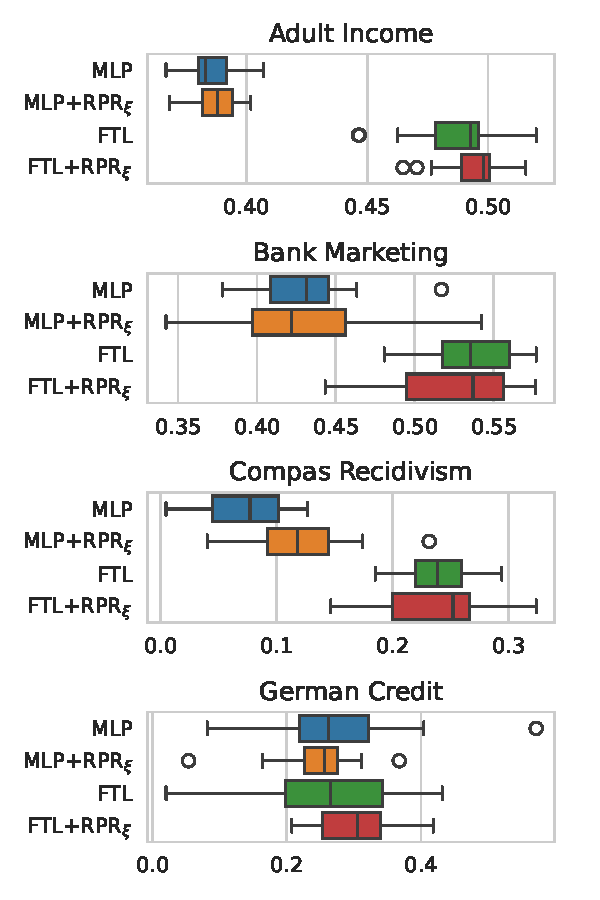
\includegraphics[width=1\linewidth]{images/boxplot_mcc_parity_rpr.pdf}
\end{subfigure}
\begin{subfigure}{.32\linewidth}
    \caption{Equal Opportunity}
    \label{fig:boxplot_mcc_opp_rpr}
    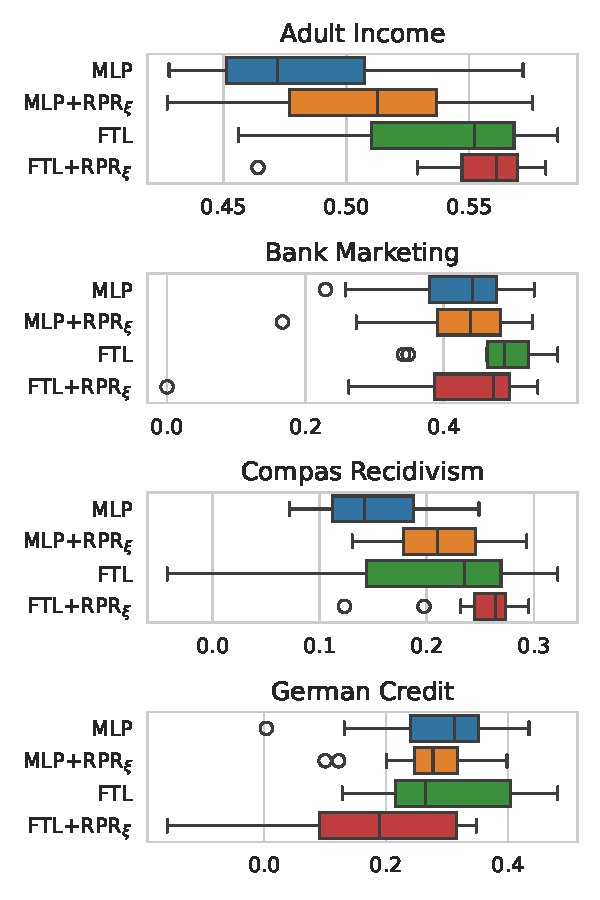
\includegraphics[width=1\linewidth]{images/boxplot_mcc_opportunity_rpr.pdf}
\end{subfigure}
\begin{subfigure}{.32\linewidth}
    \caption{Equalized Odds}
    \label{fig:boxplot_mcc_odds_rpr}
    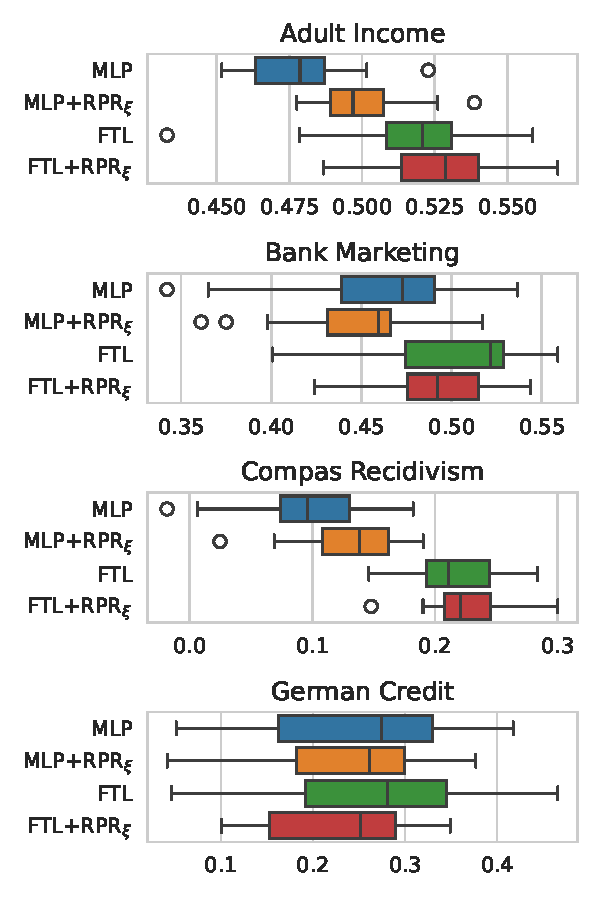
\includegraphics[width=1\linewidth]{images/boxplot_mcc_odds_rpr.pdf}
\end{subfigure}
\end{figure}

\begin{figure}[!ht]
\centering
\caption{Fitness values of RPR optimizing Accuracy and multiple fairness metrics.}\label{fig:boxplot_acc_rpr}
\begin{subfigure}{.32\linewidth}
    \caption{Statistical Parity}
    \label{fig:boxplot_acc_parity_rpr}
    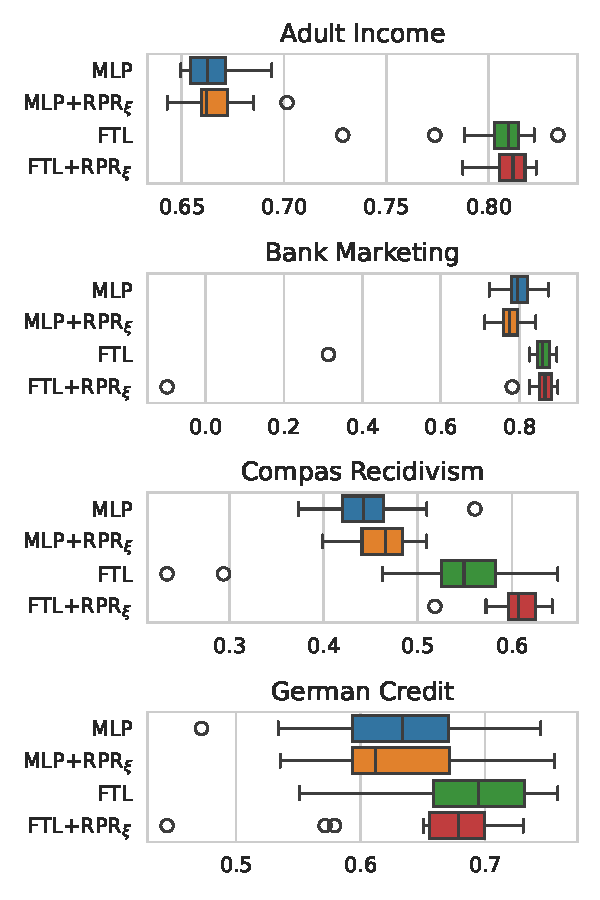
\includegraphics[width=1\linewidth]{images/boxplot_acc_parity_rpr.pdf}
\end{subfigure}
\begin{subfigure}{.32\linewidth}
    \caption{Equal Opportunity}
    \label{fig:boxplot_acc_opp_rpr}
    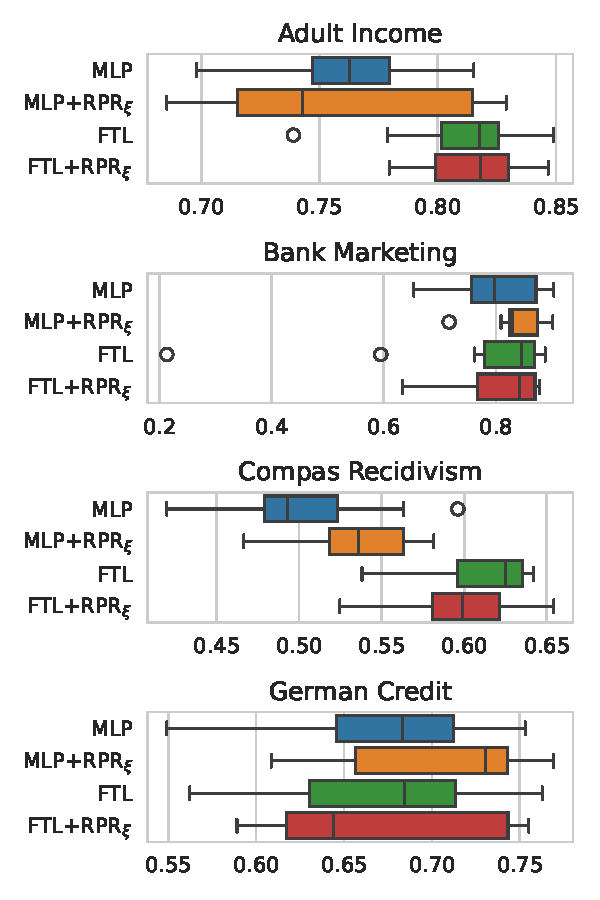
\includegraphics[width=1\linewidth]{images/boxplot_acc_opportunity_rpr.pdf}
\end{subfigure}
\begin{subfigure}{.32\linewidth}
    \caption{Equalized Odds}
    \label{fig:boxplot_acc_odds_rpr}
    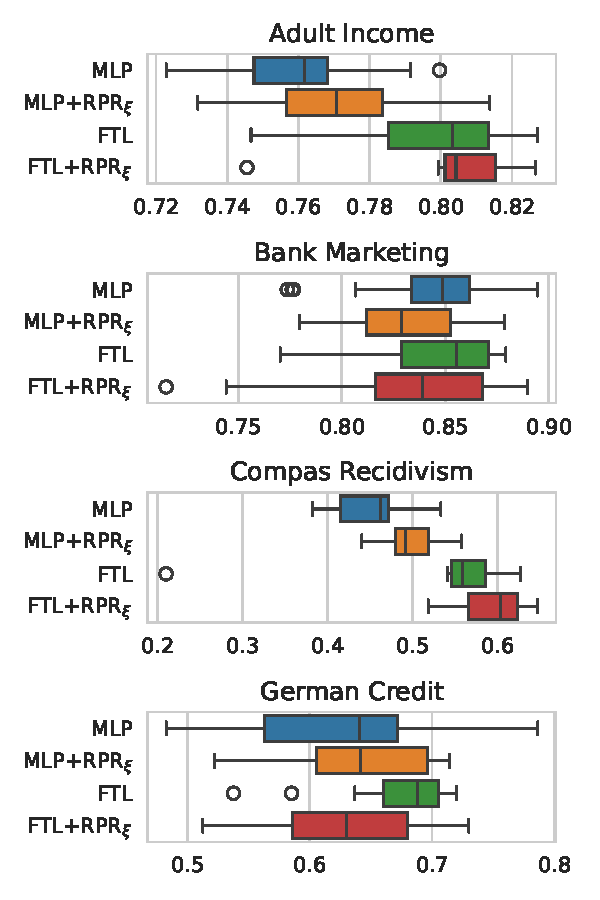
\includegraphics[width=1\linewidth]{images/boxplot_acc_odds_rpr.pdf}
\end{subfigure}
\end{figure}

Now we compare the effects of Redlining Penalty Regularizer on both MLP with standard cross entropy loss and fair transition loss. The MLP baseline here is the same presented on the last comparison (Table~\ref{tab:aso_compare_rpr_variations}), and the FTL model uses the same MLP architecture. The overall methodology remains the same, including $15$ runs with dataset resampling with $100$ trials to hyperparameter tuning each, according Table~\ref{tab:hyperparameters_rpr}. The FTL model without RPR is exactly that same presented at Chapter~\ref{chap:ftl} and on \cite{Canalli2024}, whose achieved state-of-art results. In order to provide a straightforward comparison we include only RPR$_\xi$, as it reaches the best results when compared with the others. The ASO results are available at Table~\ref{tab:aso_compare_rpr} and the box-plot comparison at Figure~\ref{fig:boxplot_mcc_rpr} and Figure~\ref{fig:boxplot_acc_rpr}.

As an additional resource to interpret these results we plot at Figure~\ref{fig:datasets_correlation} the correlations of each feature to the sensitive to each described correlation coefficient at each dataset. The correlation values are presented from highest value to the lower, to provide a non-ascendant visualization. Also, we omit the correlation of sensitive feature to it self (always $1.0$) and plot both the top $10$ correlations and the values to each feature, according the number of features at corresponding dataset. Note that Chatterjee's performs very differently when compared to the others, identifying more highly correlation values, demonstrating the functional relationship of many features with the sensitive and therefore theirs potential to be used as proxy features by the model. Another relevant perception is that the \textit{Bank dataset} presents considerably lower correlations, although still very high values than the others.  

\begin{figure}[!ht]
\centering
\caption{Sorted feature's correlation to the sensitive one according multiple correlation coefficients to all datasets.}\label{fig:datasets_correlation}
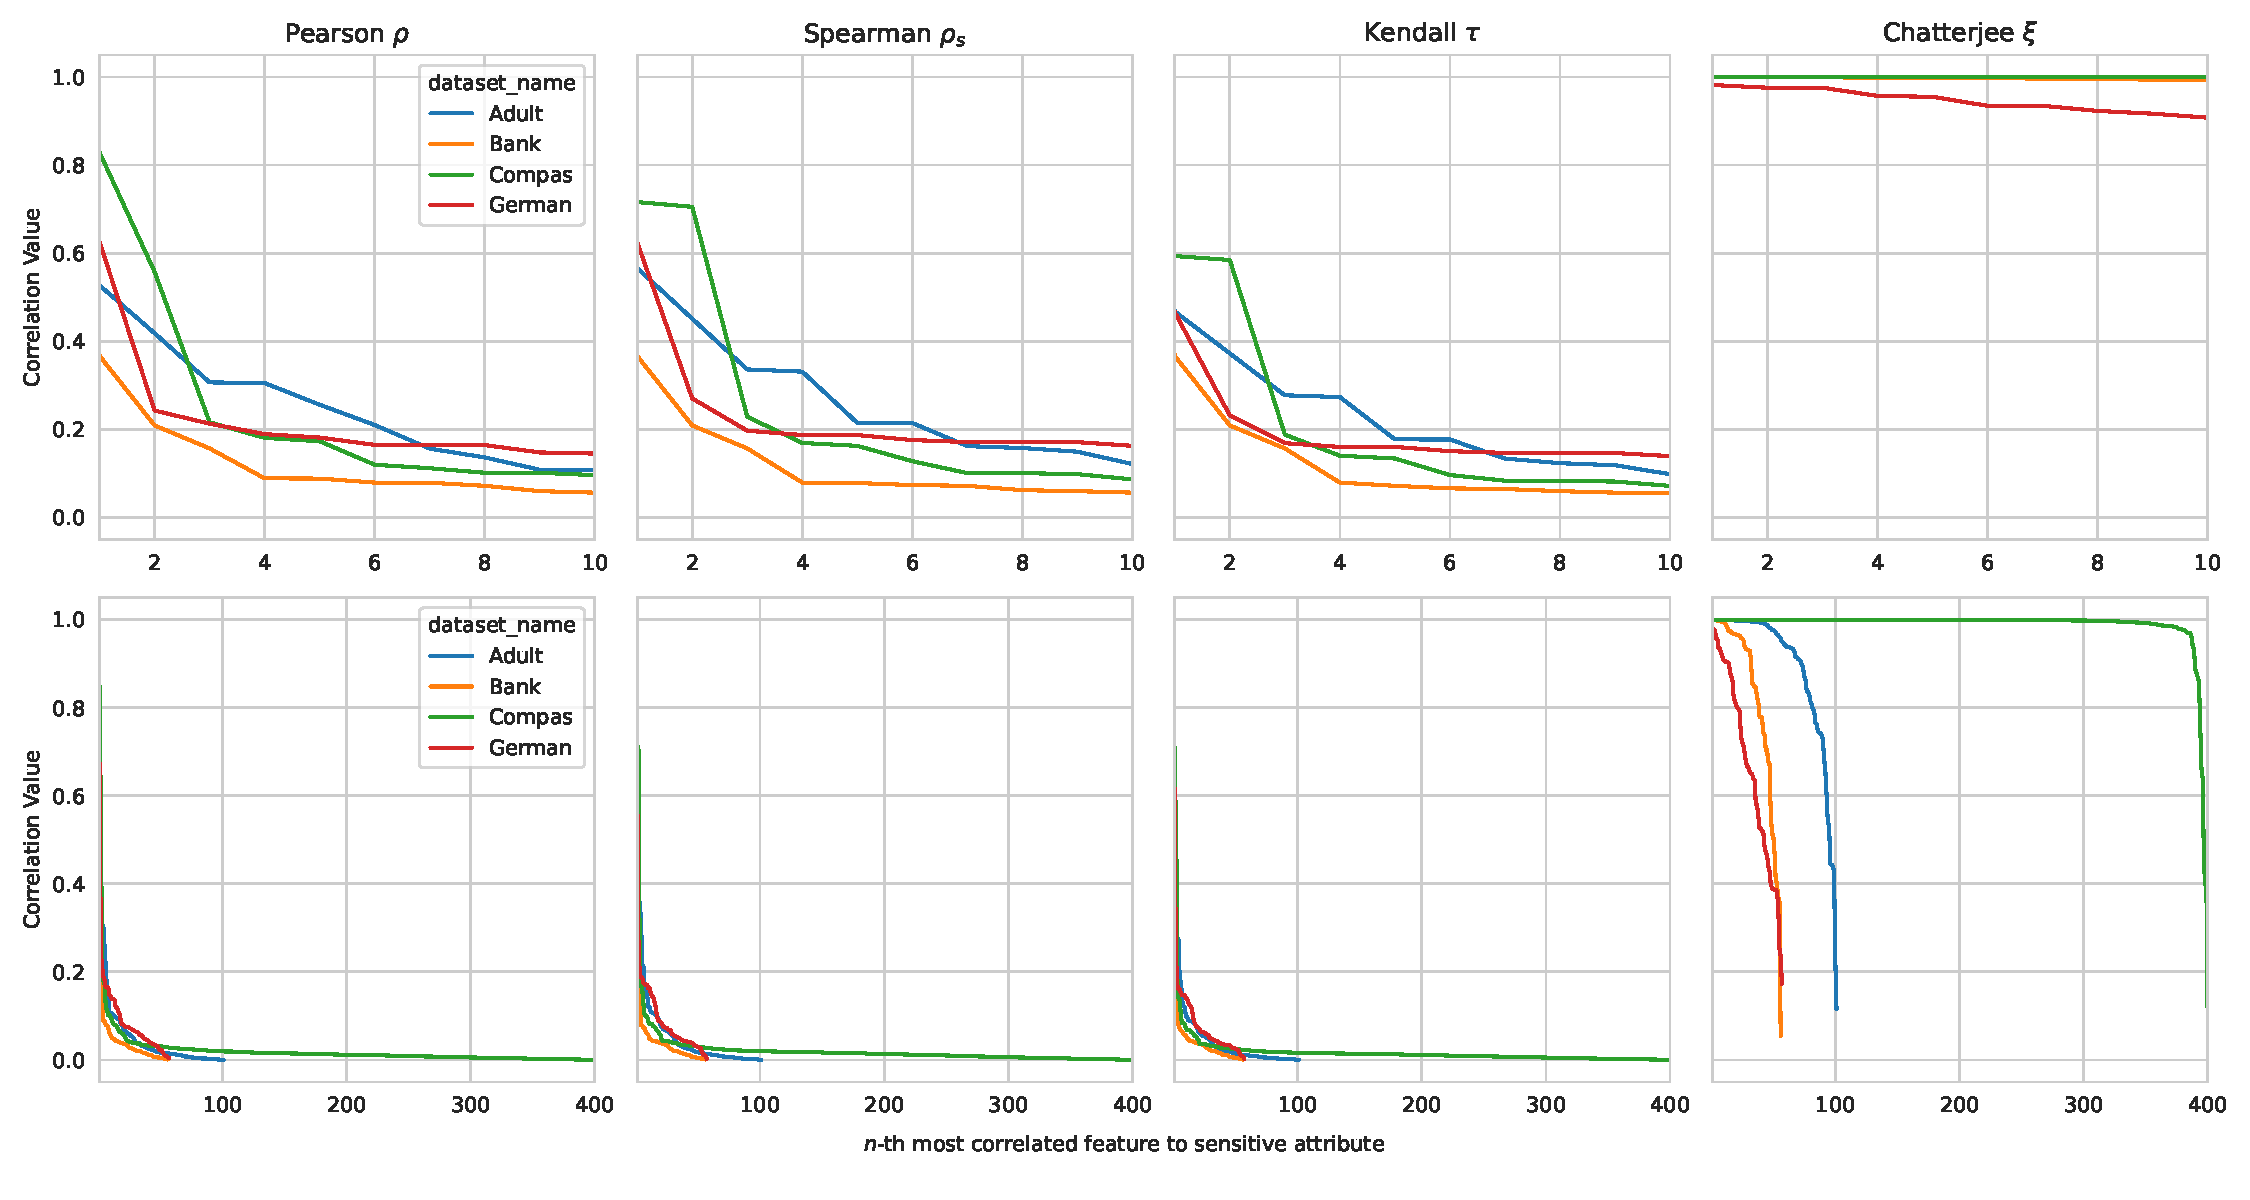
\includegraphics[width=1\linewidth]{images/dataset_correlation_plots.pdf}
\end{figure}

On Table~\ref{tab:aso_compare_rpr} RPR presents low ASO values in many scenarios, on which we can claim that it outperforms the corresponding model without penalty. It is clear that both MLP and FTL benefit with the use of RPR, whose results remains strongly better to most of optimization objectives. Here the main difference is the dataset. While to \textit{Adult} and \textit{COMPAS} the model with RPR consistently outperforms its counterparts, this not happens when the proposed technique is evaluated on \textit{Bank} and \textit{German} datasets. As referred before, \textit{German Credit} is a very small and simple dataset. In this condition the Pareto frontier is rapidly achieved, with no room left for improvement. This condition clear looking at at Figure~\ref{fig:boxplot_mcc_rpr} and Figure~\ref{fig:boxplot_acc_rpr}.  

Additionally, when comparing \textit{Bank}'s features correlations to sensitive at Figure~\ref{fig:datasets_correlation} we can argue that as it presents reduced redlining effect, the effectiveness of the proposed penalty strategy is also reduced. Analogously, the best RPR results are those assessed on \textit{COMPAS}, the dataset with the most aggressive redlining effect.

Thus, on those conditions where the dataset presents features with high potential to be learned as proxy to the sensitive feature by the model, Redlining Penalty Regularizer consistently outperforms the model without regularization. This happens to both MLP models, the one using standard cross entropy loss and with Fair Transition Loss. In this last scenario the state-of-art results described before are enhanced.

As done on the last chapter, we present performance and fairness results along with the fitness, in order to provide material to a trade-off analysis. Those metric values enable the reader to compare this results with different experimental setup and fitness objective from literature. Results corresponding each optimization scenario can be found on tables \ref{tab:complete_mcc_parity_rpr} to \ref{tab:complete_acc_odds_rpr}, presenting metric means and standard deviation values across multiple resample run. Best result of each metric within evaluation scenario are in bold, and standard deviation values are presented between parenthesis. Up arrow ($\uparrow$) indicates that the referred metric should be maximized while down arrow ($\downarrow$) that the metric should be minimized. To provide a visual resource to this comparison, the distribution of those metrics across multiple resample runs comparing the Redlining Penalty Regularization using Chatterjee's correlation (FTL) on baseline (MLP) and Fair Transition Loss (FTL) are presented in joint plot format in figures \ref{fig:complete_mcc_parity_rpr} to \ref{fig:complete_acc_odds_rpr}. Each joint plot is present within the corresponding table to a better comprehension.

\newpage

\begin{table}
    \centering
    \caption{Mean and standard deviation metric values optimizing MCC and Statistical Parity in comparison with Redlining Penalty Regularizer.}\label{tab:complete_mcc_parity_rpr}
    {\tiny\begin{tabular}{llrrr}
    \toprule
    Dataset & Method & $\uparrow\;$Fitness & $\uparrow\;$MCC & $\downarrow\;$Stat. Parity \\
    \midrule
    \multirow{8}{*}{\shortstack[l]{Adult\\ Income}} & FTL & $0.487 \; (\pm0.02)$ & $0.509 \; (\pm0.02)$ & $\textbf{0.022} \; (\pm0.02)$ \\
     & FTL+RPR$_{\xi}$ & $\textbf{0.494} \; (\pm0.01)$ & $0.517 \; (\pm0.02)$ & $0.023 \; (\pm0.02)$ \\
     & MLP & $0.386 \; (\pm0.01)$ & $0.576 \; (\pm0.01)$ & $0.191 \; (\pm0.01)$ \\
     & MLP+L2 & $0.385 \; (\pm0.01)$ & $0.576 \; (\pm0.01)$ & $0.190 \; (\pm0.01)$ \\
     & MLP+RPR$_{\rho_s}$ & $0.384 \; (\pm0.01)$ & $0.576 \; (\pm0.01)$ & $0.192 \; (\pm0.01)$ \\
     & MLP+RPR$_{\rho}$ & $0.393 \; (\pm0.01)$ & $\textbf{0.580} \; (\pm0.01)$ & $0.187 \; (\pm0.01)$ \\
     & MLP+RPR$_{\tau}$ & $0.386 \; (\pm0.01)$ & $0.577 \; (\pm0.01)$ & $0.191 \; (\pm0.01)$ \\
     & MLP+RPR$_{\xi}$ & $0.388 \; (\pm0.01)$ & $0.578 \; (\pm0.01)$ & $0.191 \; (\pm0.01)$ \\
    \midrule
    \multirow{8}{*}{\shortstack[l]{Bank\\ Marketing}} & FTL & $\textbf{0.534} \; (\pm0.03)$ & $\textbf{0.569} \; (\pm0.01)$ & $\textbf{0.035} \; (\pm0.03)$ \\
     & FTL+RPR$_{\xi}$ & $0.523 \; (\pm0.04)$ & $\textbf{0.569} \; (\pm0.01)$ & $0.046 \; (\pm0.04)$ \\
     & MLP & $0.429 \; (\pm0.03)$ & $0.521 \; (\pm0.02)$ & $0.092 \; (\pm0.02)$ \\
     & MLP+L2 & $0.412 \; (\pm0.04)$ & $0.521 \; (\pm0.02)$ & $0.110 \; (\pm0.03)$ \\
     & MLP+RPR$_{\rho_s}$ & $0.422 \; (\pm0.03)$ & $0.527 \; (\pm0.02)$ & $0.106 \; (\pm0.03)$ \\
     & MLP+RPR$_{\rho}$ & $0.424 \; (\pm0.03)$ & $0.523 \; (\pm0.01)$ & $0.100 \; (\pm0.03)$ \\
     & MLP+RPR$_{\tau}$ & $0.412 \; (\pm0.04)$ & $0.520 \; (\pm0.02)$ & $0.108 \; (\pm0.03)$ \\
     & MLP+RPR$_{\xi}$ & $0.426 \; (\pm0.05)$ & $0.528 \; (\pm0.02)$ & $0.102 \; (\pm0.04)$ \\
    \midrule
    \multirow{8}{*}{\shortstack[l]{COMPAS\\ Recidivism}} & FTL & $\textbf{0.239} \; (\pm0.03)$ & $0.276 \; (\pm0.03)$ & $\textbf{0.036} \; (\pm0.03)$ \\
     & FTL+RPR$_{\xi}$ & $0.236 \; (\pm0.05)$ & $0.294 \; (\pm0.03)$ & $0.058 \; (\pm0.04)$ \\
     & MLP & $0.074 \; (\pm0.03)$ & $0.283 \; (\pm0.02)$ & $0.209 \; (\pm0.04)$ \\
     & MLP+L2 & $0.089 \; (\pm0.04)$ & $0.291 \; (\pm0.02)$ & $0.202 \; (\pm0.04)$ \\
     & MLP+RPR$_{\rho_s}$ & $0.083 \; (\pm0.05)$ & $0.293 \; (\pm0.03)$ & $0.210 \; (\pm0.04)$ \\
     & MLP+RPR$_{\rho}$ & $0.087 \; (\pm0.05)$ & $0.282 \; (\pm0.03)$ & $0.195 \; (\pm0.04)$ \\
     & MLP+RPR$_{\tau}$ & $0.085 \; (\pm0.03)$ & $0.281 \; (\pm0.02)$ & $0.197 \; (\pm0.03)$ \\
     & MLP+RPR$_{\xi}$ & $0.121 \; (\pm0.05)$ & $\textbf{0.329} \; (\pm0.03)$ & $0.208 \; (\pm0.03)$ \\
    \midrule
    \multirow{8}{*}{\shortstack[l]{German\\ Credit}} & FTL & $0.256 \; (\pm0.12)$ & $0.355 \; (\pm0.08)$ & $0.099 \; (\pm0.06)$ \\
     & FTL+RPR$_{\xi}$ & $\textbf{0.302} \; (\pm0.06)$ & $0.371 \; (\pm0.05)$ & $0.069 \; (\pm0.05)$ \\
     & MLP & $0.266 \; (\pm0.10)$ & $0.329 \; (\pm0.09)$ & $\textbf{0.064} \; (\pm0.05)$ \\
     & MLP+L2 & $0.261 \; (\pm0.10)$ & $\textbf{0.374} \; (\pm0.09)$ & $0.113 \; (\pm0.07)$ \\
     & MLP+RPR$_{\rho_s}$ & $0.192 \; (\pm0.11)$ & $0.292 \; (\pm0.07)$ & $0.099 \; (\pm0.06)$ \\
     & MLP+RPR$_{\rho}$ & $0.255 \; (\pm0.07)$ & $0.341 \; (\pm0.07)$ & $0.087 \; (\pm0.04)$ \\
     & MLP+RPR$_{\tau}$ & $0.256 \; (\pm0.08)$ & $0.342 \; (\pm0.05)$ & $0.086 \; (\pm0.06)$ \\
     & MLP+RPR$_{\xi}$ & $0.246 \; (\pm0.07)$ & $0.329 \; (\pm0.05)$ & $0.084 \; (\pm0.06)$ \\
    \bottomrule
\end{tabular}}
\end{table}

\begin{figure}
\centering
\caption{Metric distribution optimizing MCC and Statistical Parity in comparison with Redlining Penalty Regularization across multiple resample runs. Corresponding values available at Table~\ref{tab:complete_mcc_parity_rpr}.}
\label{fig:complete_mcc_parity_rpr}
\begin{subfigure}{.45\linewidth}
    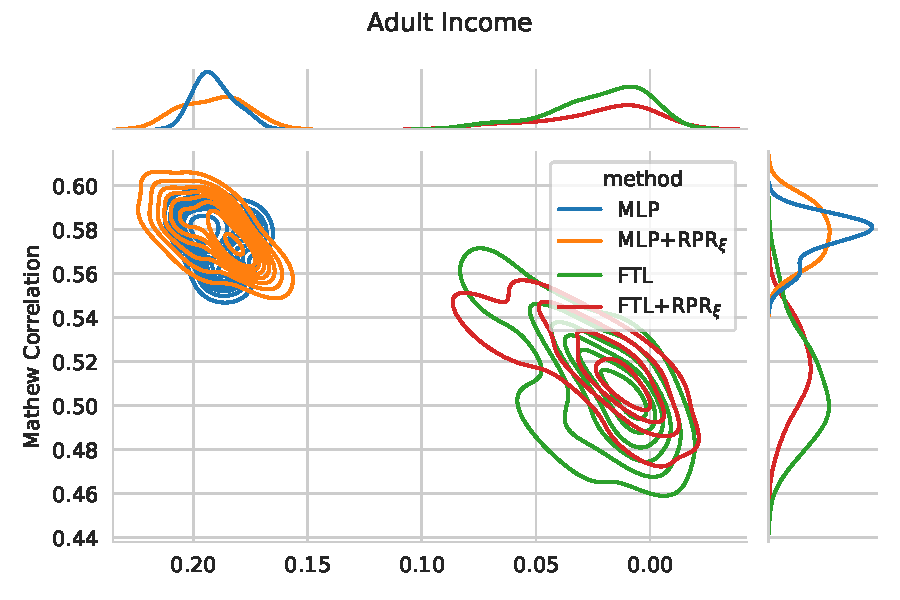
\includegraphics[width=1\linewidth]{images/pareto_mcc_parity_adult_rpr.pdf}
\end{subfigure}
\begin{subfigure}{.45\linewidth}
    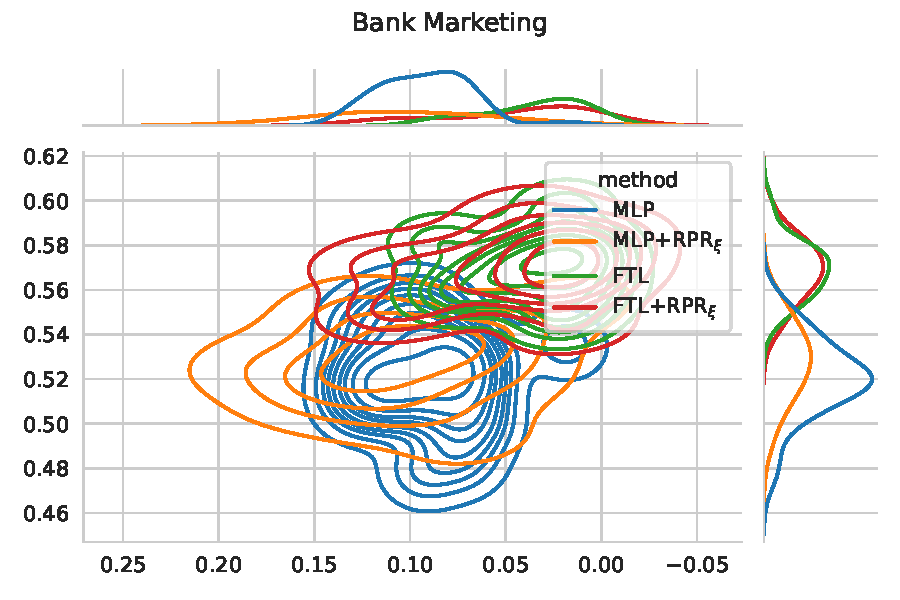
\includegraphics[width=1\linewidth]{images/pareto_mcc_parity_bank_rpr.pdf}
\end{subfigure}

\begin{subfigure}{.45\linewidth}
    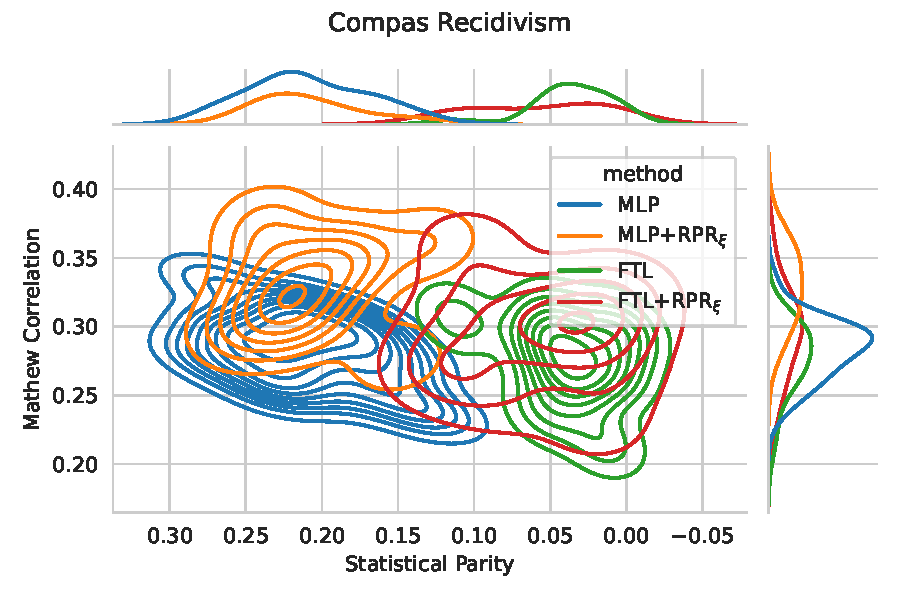
\includegraphics[width=1\linewidth]{images/pareto_mcc_parity_compas_rpr.pdf}
\end{subfigure}
\begin{subfigure}{.45\linewidth}
    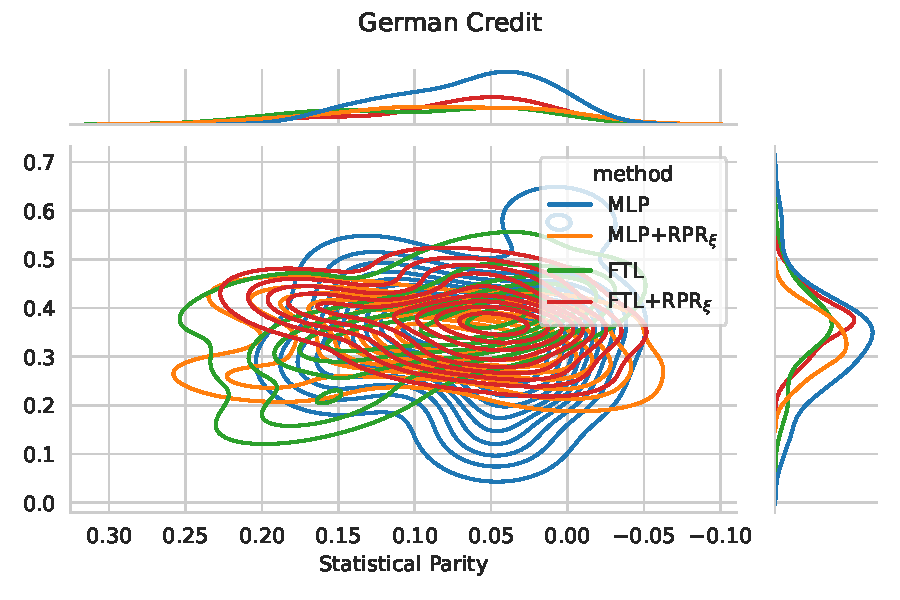
\includegraphics[width=1\linewidth]{images/pareto_mcc_parity_german_rpr.pdf}
\end{subfigure}
\end{figure}

 \begin{table}
    \centering
    \caption{Mean and standard deviation metric values optimizing MCC and Equal Opportunity in comparison with Redlining Penalty Regularizer.}\label{tab:complete_mcc_opportunity_rpr}
    {\tiny\begin{tabular}{llrrr}
    \toprule
    Dataset & Method & $\uparrow\;$Fitness & $\uparrow\;$MCC & $\downarrow\;$Eq. Opp. \\
    \midrule
    
    \multirow{8}{*}{\shortstack[l]{Adult\\ Income}} & FTL & $0.540 \; (\pm0.04)$ & $0.576 \; (\pm0.01)$ & $0.036 \; (\pm0.03)$ \\
     & FTL+RPR$_{\xi}$ & $\textbf{0.554} \; (\pm0.03)$ & $0.581 \; (\pm0.02)$ & $\textbf{0.027} \; (\pm0.02)$ \\
     & MLP & $0.480 \; (\pm0.04)$ & $\textbf{0.582} \; (\pm0.01)$ & $0.103 \; (\pm0.04)$ \\
     & MLP+L2 & $0.479 \; (\pm0.03)$ & $0.580 \; (\pm0.01)$ & $0.102 \; (\pm0.03)$ \\
     & MLP+RPR$_{\rho_s}$ & $0.493 \; (\pm0.04)$ & $0.578 \; (\pm0.01)$ & $0.085 \; (\pm0.04)$ \\
     & MLP+RPR$_{\rho}$ & $0.478 \; (\pm0.04)$ & $0.580 \; (\pm0.01)$ & $0.102 \; (\pm0.04)$ \\
     & MLP+RPR$_{\tau}$ & $0.488 \; (\pm0.04)$ & $0.580 \; (\pm0.01)$ & $0.092 \; (\pm0.03)$ \\
     & MLP+RPR$_{\xi}$ & $0.506 \; (\pm0.05)$ & $0.577 \; (\pm0.01)$ & $0.071 \; (\pm0.05)$ \\
    \midrule
    \multirow{8}{*}{\shortstack[l]{Bank\\ Marketing}} & FTL & $\textbf{0.483} \; (\pm0.07)$ & $\textbf{0.567} \; (\pm0.02)$ & $0.084 \; (\pm0.06)$ \\
     & FTL+RPR$_{\xi}$ & $0.416 \; (\pm0.14)$ & $0.519 \; (\pm0.15)$ & $0.104 \; (\pm0.08)$ \\
     & MLP & $0.420 \; (\pm0.08)$ & $0.524 \; (\pm0.02)$ & $0.104 \; (\pm0.08)$ \\
     & MLP+L2 & $0.438 \; (\pm0.06)$ & $0.514 \; (\pm0.02)$ & $0.076 \; (\pm0.06)$ \\
     & MLP+RPR$_{\rho_s}$ & $0.426 \; (\pm0.06)$ & $0.520 \; (\pm0.02)$ & $0.094 \; (\pm0.06)$ \\
     & MLP+RPR$_{\rho}$ & $0.452 \; (\pm0.05)$ & $0.527 \; (\pm0.02)$ & $\textbf{0.074} \; (\pm0.05)$ \\
     & MLP+RPR$_{\tau}$ & $0.417 \; (\pm0.08)$ & $0.526 \; (\pm0.02)$ & $0.109 \; (\pm0.07)$ \\
     & MLP+RPR$_{\xi}$ & $0.420 \; (\pm0.10)$ & $0.529 \; (\pm0.02)$ & $0.109 \; (\pm0.09)$ \\
    \midrule
    \multirow{8}{*}{\shortstack[l]{COMPAS\\ Recidivism}} & FTL & $0.195 \; (\pm0.11)$ & $0.281 \; (\pm0.03)$ & $0.086 \; (\pm0.09)$ \\
     & FTL+RPR$_{\xi}$ & $\textbf{0.251} \; (\pm0.04)$ & $0.309 \; (\pm0.03)$ & $\textbf{0.058} \; (\pm0.04)$ \\
     & MLP & $0.150 \; (\pm0.05)$ & $0.282 \; (\pm0.03)$ & $0.132 \; (\pm0.05)$ \\
     & MLP+L2 & $0.146 \; (\pm0.06)$ & $0.282 \; (\pm0.03)$ & $0.136 \; (\pm0.04)$ \\
     & MLP+RPR$_{\rho_s}$ & $0.179 \; (\pm0.04)$ & $0.303 \; (\pm0.02)$ & $0.124 \; (\pm0.03)$ \\
     & MLP+RPR$_{\rho}$ & $0.168 \; (\pm0.06)$ & $0.290 \; (\pm0.03)$ & $0.122 \; (\pm0.05)$ \\
     & MLP+RPR$_{\tau}$ & $0.146 \; (\pm0.05)$ & $0.289 \; (\pm0.03)$ & $0.143 \; (\pm0.04)$ \\
     & MLP+RPR$_{\xi}$ & $0.211 \; (\pm0.05)$ & $\textbf{0.325} \; (\pm0.02)$ & $0.114 \; (\pm0.04)$ \\
    \midrule
    \multirow{8}{*}{\shortstack[l]{German\\ Credit}} & FTL & $\textbf{0.293} \; (\pm0.12)$ & $\textbf{0.368} \; (\pm0.10)$ & $0.074 \; (\pm0.05)$ \\
     & FTL+RPR$_{\xi}$ & $0.166 \; (\pm0.16)$ & $0.284 \; (\pm0.14)$ & $0.117 \; (\pm0.07)$ \\
     & MLP & $0.290 \; (\pm0.09)$ & $0.355 \; (\pm0.07)$ & $0.065 \; (\pm0.06)$ \\
     & MLP+L2 & $0.249 \; (\pm0.08)$ & $0.309 \; (\pm0.07)$ & $0.060 \; (\pm0.04)$ \\
     & MLP+RPR$_{\rho_s}$ & $0.319 \; (\pm0.05)$ & $0.367 \; (\pm0.07)$ & $\textbf{0.048} \; (\pm0.04)$ \\
     & MLP+RPR$_{\rho}$ & $0.229 \; (\pm0.13)$ & $0.297 \; (\pm0.10)$ & $0.068 \; (\pm0.04)$ \\
     & MLP+RPR$_{\tau}$ & $0.277 \; (\pm0.08)$ & $0.329 \; (\pm0.06)$ & $0.053 \; (\pm0.04)$ \\
     & MLP+RPR$_{\xi}$ & $0.275 \; (\pm0.09)$ & $0.341 \; (\pm0.06)$ & $0.066 \; (\pm0.05)$ \\
     \bottomrule
\end{tabular}}
\end{table}

\begin{figure}
\centering
\caption{Metric distribution optimizing MCC and Equal Opportunity in comparison with Redlining Penalty Regularization across multiple resample runs. Corresponding values available at Table~\ref{tab:complete_mcc_opportunity_rpr}.}
\label{fig:complete_mcc_opportunity_rpr}
\begin{subfigure}{.45\linewidth}
    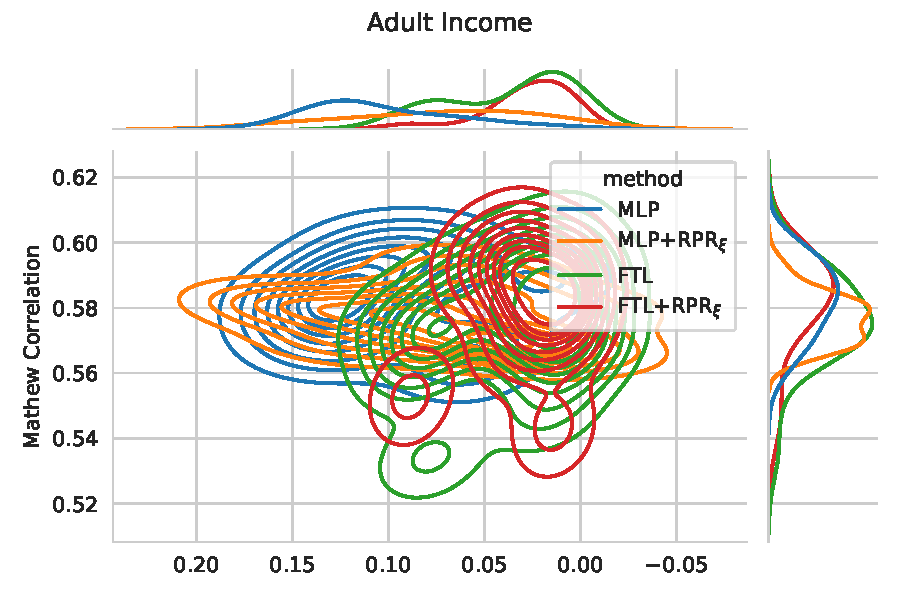
\includegraphics[width=1\linewidth]{images/pareto_mcc_opportunity_adult_rpr.pdf}
\end{subfigure}
\begin{subfigure}{.45\linewidth}
    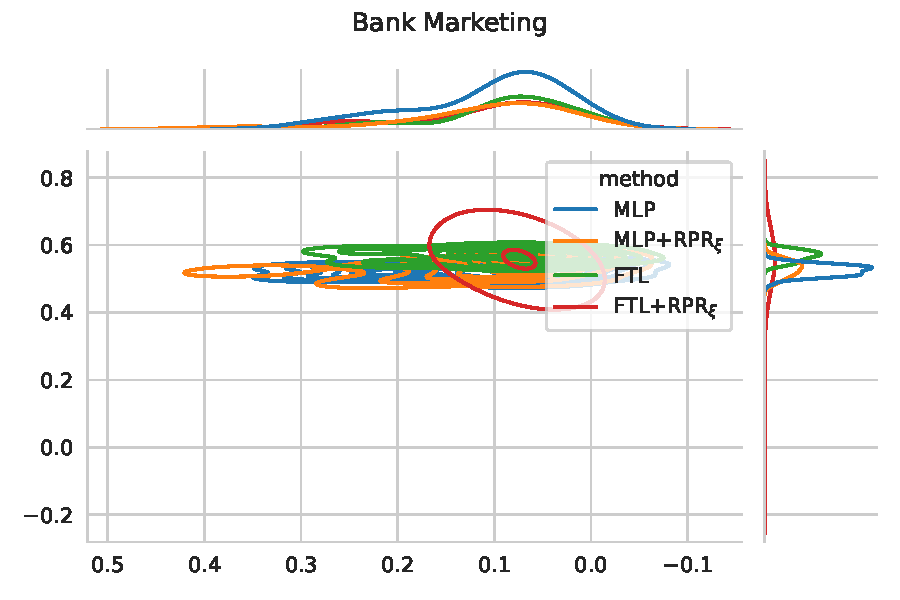
\includegraphics[width=1\linewidth]{images/pareto_mcc_opportunity_bank_rpr.pdf}
\end{subfigure}

\begin{subfigure}{.45\linewidth}
    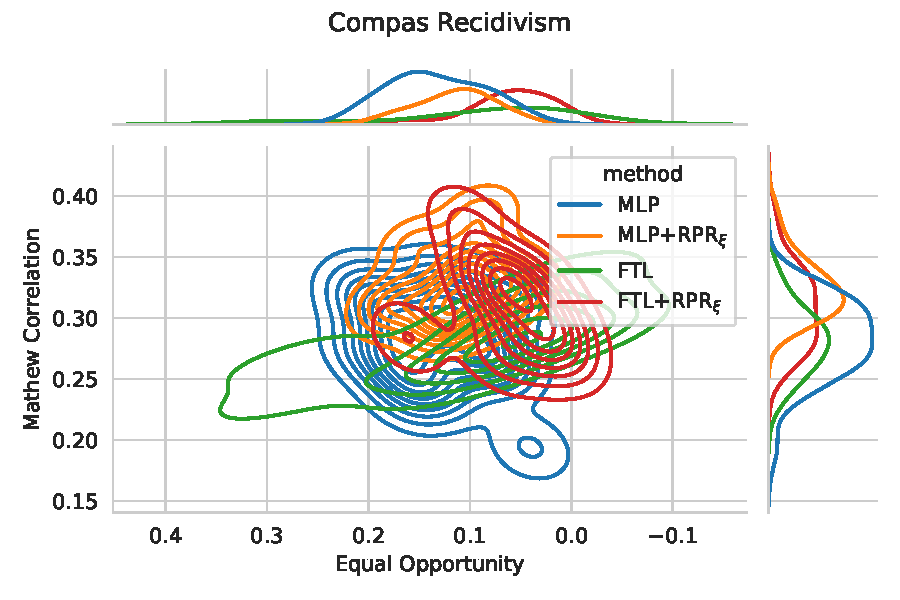
\includegraphics[width=1\linewidth]{images/pareto_mcc_opportunity_compas_rpr.pdf}
\end{subfigure}
\begin{subfigure}{.45\linewidth}
    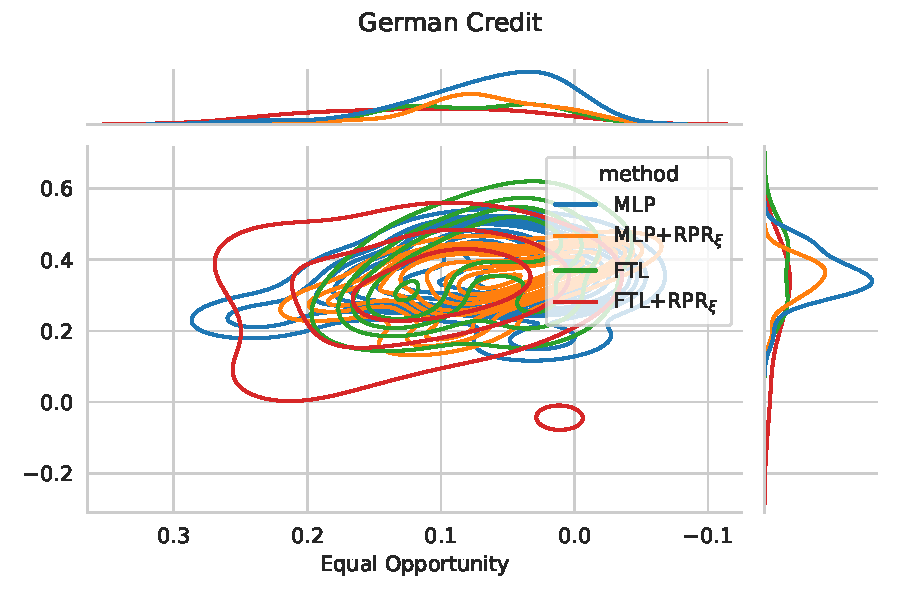
\includegraphics[width=1\linewidth]{images/pareto_mcc_opportunity_german_rpr.pdf}
\end{subfigure}
\end{figure}


 \begin{table}
    \centering
    \caption{Mean and standard deviation metric values optimizing MCC and Equalized Odds in comparison with Redlining Penalty Regularizer.}\label{tab:complete_mcc_odds_rpr}
    {\tiny\begin{tabular}{llrrr}
    \toprule
    Dataset & Method & $\uparrow\;$Fitness & $\uparrow\;$MCC & $\downarrow\;$Eq. Odds \\
    \midrule
    
    \multirow{8}{*}{\shortstack[l]{Adult\\ Income}} & FTL & $0.515 \; (\pm0.03)$ & $0.572 \; (\pm0.02)$ & $0.057 \; (\pm0.02)$ \\
     & FTL+RPR$_{\xi}$ & $\textbf{0.526} \; (\pm0.02)$ & $0.575 \; (\pm0.01)$ & $\textbf{0.048} \; (\pm0.02)$ \\
     & MLP & $0.478 \; (\pm0.02)$ & $0.575 \; (\pm0.01)$ & $0.097 \; (\pm0.02)$ \\
     & MLP+L2 & $0.484 \; (\pm0.01)$ & $0.577 \; (\pm0.01)$ & $0.093 \; (\pm0.01)$ \\
     & MLP+RPR$_{\rho_s}$ & $0.492 \; (\pm0.02)$ & $\textbf{0.578} \; (\pm0.01)$ & $0.085 \; (\pm0.02)$ \\
     & MLP+RPR$_{\rho}$ & $0.489 \; (\pm0.02)$ & $0.575 \; (\pm0.01)$ & $0.087 \; (\pm0.02)$ \\
     & MLP+RPR$_{\tau}$ & $0.487 \; (\pm0.02)$ & $\textbf{0.578} \; (\pm0.01)$ & $0.091 \; (\pm0.02)$ \\
     & MLP+RPR$_{\xi}$ & $0.500 \; (\pm0.02)$ & $\textbf{0.578} \; (\pm0.01)$ & $0.078 \; (\pm0.02)$ \\
    \midrule
    \multirow{8}{*}{\shortstack[l]{Bank\\ Marketing}} & FTL & $\textbf{0.495} \; (\pm0.05)$ & $\textbf{0.574} \; (\pm0.01)$ & $0.078 \; (\pm0.05)$ \\
     & FTL+RPR$_{\xi}$ & $0.490 \; (\pm0.03)$ & $0.571 \; (\pm0.01)$ & $0.081 \; (\pm0.03)$ \\
     & MLP & $0.461 \; (\pm0.05)$ & $0.522 \; (\pm0.02)$ & $\textbf{0.061} \; (\pm0.04)$ \\
     & MLP+L2 & $0.461 \; (\pm0.03)$ & $0.525 \; (\pm0.02)$ & $0.065 \; (\pm0.03)$ \\
     & MLP+RPR$_{\rho_s}$ & $0.468 \; (\pm0.04)$ & $0.529 \; (\pm0.02)$ & $\textbf{0.061} \; (\pm0.03)$ \\
     & MLP+RPR$_{\rho}$ & $0.442 \; (\pm0.05)$ & $0.522 \; (\pm0.02)$ & $0.080 \; (\pm0.03)$ \\
     & MLP+RPR$_{\tau}$ & $0.434 \; (\pm0.05)$ & $0.519 \; (\pm0.01)$ & $0.085 \; (\pm0.05)$ \\
     & MLP+RPR$_{\xi}$ & $0.446 \; (\pm0.04)$ & $0.539 \; (\pm0.02)$ & $0.093 \; (\pm0.04)$ \\
    \midrule
    \multirow{8}{*}{\shortstack[l]{COMPAS\\ Recidivism}} & FTL & $0.216 \; (\pm0.04)$ & $0.288 \; (\pm0.02)$ & $0.072 \; (\pm0.04)$ \\
     & FTL+RPR$_{\xi}$ & $\textbf{0.225} \; (\pm0.04)$ & $0.282 \; (\pm0.03)$ & $\textbf{0.056} \; (\pm0.03)$ \\
     & MLP & $0.098 \; (\pm0.05)$ & $0.283 \; (\pm0.03)$ & $0.185 \; (\pm0.03)$ \\
     & MLP+L2 & $0.097 \; (\pm0.04)$ & $0.281 \; (\pm0.03)$ & $0.185 \; (\pm0.04)$ \\
     & MLP+RPR$_{\rho_s}$ & $0.096 \; (\pm0.05)$ & $0.282 \; (\pm0.03)$ & $0.185 \; (\pm0.03)$ \\
     & MLP+RPR$_{\rho}$ & $0.119 \; (\pm0.05)$ & $0.292 \; (\pm0.03)$ & $0.174 \; (\pm0.03)$ \\
     & MLP+RPR$_{\tau}$ & $0.124 \; (\pm0.04)$ & $\textbf{0.310} \; (\pm0.02)$ & $0.185 \; (\pm0.03)$ \\
     & MLP+RPR$_{\xi}$ & $0.129 \; (\pm0.05)$ & $0.303 \; (\pm0.02)$ & $0.174 \; (\pm0.03)$ \\
    \midrule
    \multirow{8}{*}{\shortstack[l]{German\\ Credit}} & FTL & $\textbf{0.278} \; (\pm0.12)$ & $\textbf{0.383} \; (\pm0.08)$ & $0.105 \; (\pm0.06)$ \\
     & FTL+RPR$_{\xi}$ & $0.228 \; (\pm0.08)$ & $0.337 \; (\pm0.07)$ & $0.109 \; (\pm0.06)$ \\
     & MLP & $0.249 \; (\pm0.10)$ & $0.352 \; (\pm0.08)$ & $0.102 \; (\pm0.06)$ \\
     & MLP+L2 & $0.214 \; (\pm0.11)$ & $0.297 \; (\pm0.10)$ & $\textbf{0.084} \; (\pm0.05)$ \\
     & MLP+RPR$_{\rho_s}$ & $0.219 \; (\pm0.09)$ & $0.352 \; (\pm0.07)$ & $0.133 \; (\pm0.05)$ \\
     & MLP+RPR$_{\rho}$ & $0.228 \; (\pm0.11)$ & $0.342 \; (\pm0.06)$ & $0.114 \; (\pm0.09)$ \\
     & MLP+RPR$_{\tau}$ & $0.247 \; (\pm0.06)$ & $0.341 \; (\pm0.06)$ & $0.094 \; (\pm0.05)$ \\
     & MLP+RPR$_{\xi}$ & $0.231 \; (\pm0.10)$ & $0.332 \; (\pm0.07)$ & $0.102 \; (\pm0.06)$ \\
     \bottomrule
\end{tabular}}
\end{table}

\begin{figure}
\centering
\caption{Metric distribution optimizing MCC and Equalized Odds in comparison with Redlining Penalty Regularization across multiple resample runs. Corresponding values available at Table~\ref{tab:complete_mcc_odds_rpr}.}
\label{fig:complete_mcc_odds_rpr}
\begin{subfigure}{.45\linewidth}
    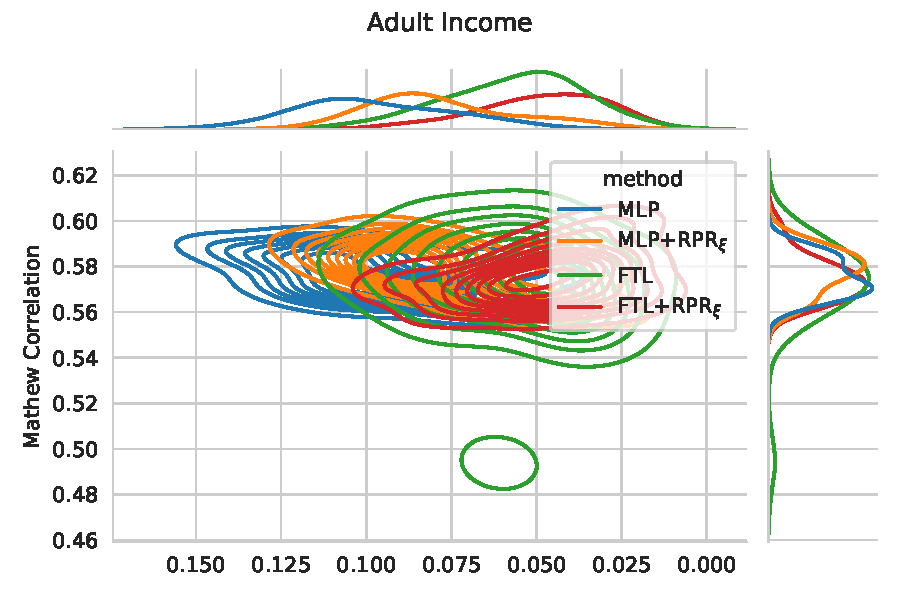
\includegraphics[width=1\linewidth]{images/pareto_mcc_odds_adult_rpr.pdf}
\end{subfigure}
\begin{subfigure}{.45\linewidth}
    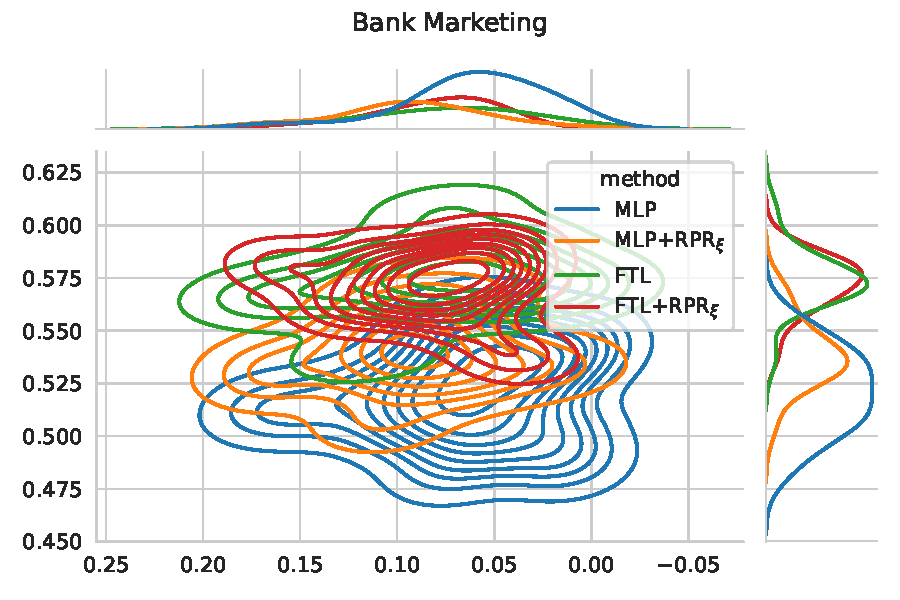
\includegraphics[width=1\linewidth]{images/pareto_mcc_odds_bank_rpr.pdf}
\end{subfigure}

\begin{subfigure}{.45\linewidth}
    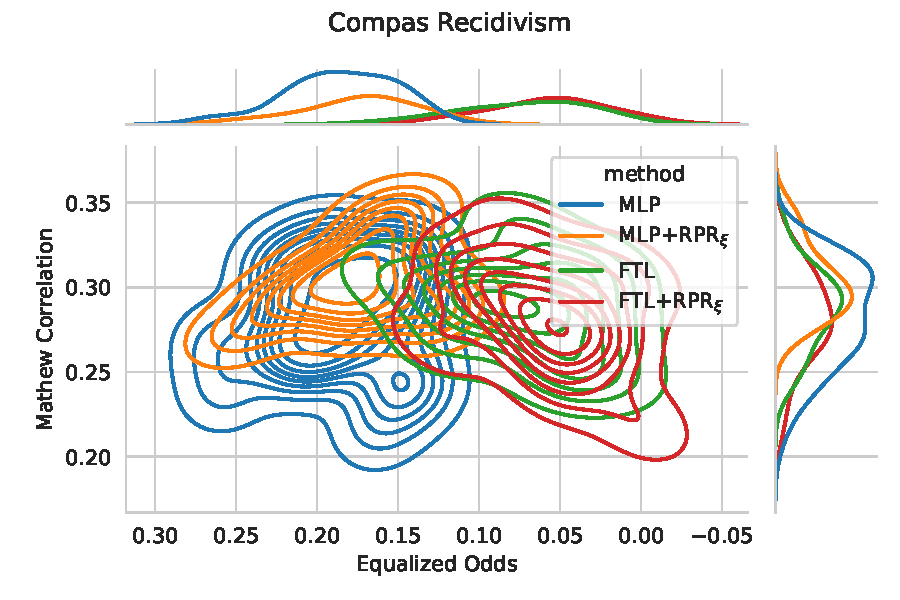
\includegraphics[width=1\linewidth]{images/pareto_mcc_odds_compas_rpr.pdf}
\end{subfigure}
\begin{subfigure}{.45\linewidth}
    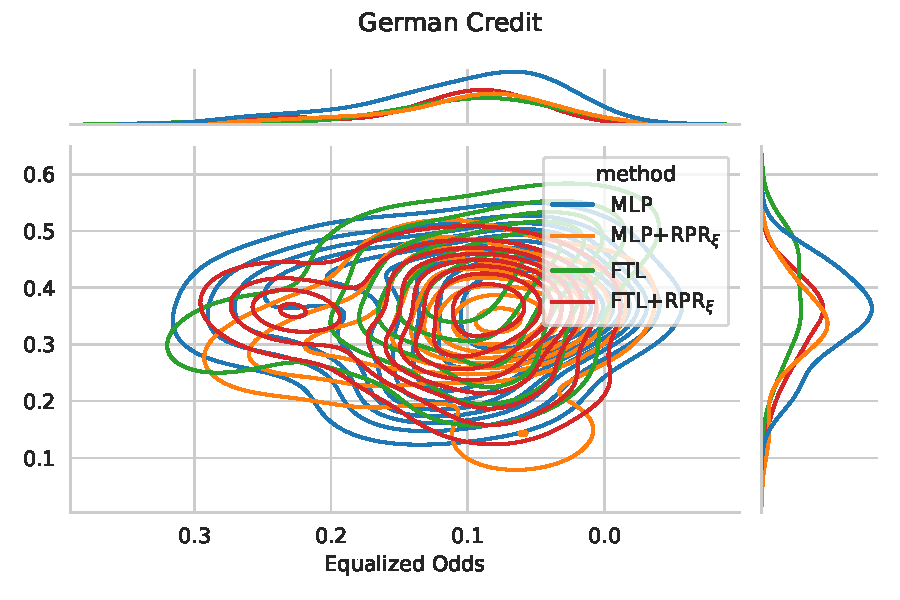
\includegraphics[width=1\linewidth]{images/pareto_mcc_odds_german_rpr.pdf}
\end{subfigure}
\end{figure}

 \begin{table}
    \centering
    \caption{Mean and standard deviation metric values optimizing Accuracy and Statistical Parity in comparison with Redlining Penalty Regularizer.}\label{tab:complete_acc_parity_rpr}
   {\tiny \begin{tabular}{llrrr}
    \toprule
    Dataset & Method & $\uparrow\;$Fitness & $\uparrow\;$Accuracy & $\downarrow\;$Stat. Parity \\
    \midrule
    
    \multirow{8}{*}{\shortstack[l]{Adult\\ Income}} & FTL & $0.806 \; (\pm0.02)$ & $0.827 \; (\pm0.01)$ & $0.022 \; (\pm0.02)$ \\
     & FTL+RPR$_{\xi}$ & $\textbf{0.811} \; (\pm0.01)$ & $0.825 \; (\pm0.01)$ & $\textbf{0.015} \; (\pm0.01)$ \\
     & MLP & $0.664 \; (\pm0.01)$ & $0.850 \; (\pm0.00)$ & $0.185 \; (\pm0.01)$ \\
     & MLP+L2 & $0.660 \; (\pm0.01)$ & $\textbf{0.851} \; (\pm0.00)$ & $0.191 \; (\pm0.01)$ \\
     & MLP+RPR$_{\rho_s}$ & $0.663 \; (\pm0.01)$ & $0.848 \; (\pm0.00)$ & $0.186 \; (\pm0.01)$ \\
     & MLP+RPR$_{\rho}$ & $0.657 \; (\pm0.01)$ & $0.849 \; (\pm0.00)$ & $0.192 \; (\pm0.01)$ \\
     & MLP+RPR$_{\tau}$ & $0.659 \; (\pm0.01)$ & $0.849 \; (\pm0.00)$ & $0.190 \; (\pm0.01)$ \\
     & MLP+RPR$_{\xi}$ & $0.666 \; (\pm0.01)$ & $0.850 \; (\pm0.00)$ & $0.183 \; (\pm0.02)$ \\
    \midrule
    \multirow{8}{*}{\shortstack[l]{Bank\\ Marketing}} & FTL & $\textbf{0.828} \; (\pm0.14)$ & $0.887 \; (\pm0.01)$ & $\textbf{0.059} \; (\pm0.14)$ \\
     & FTL+RPR$_{\xi}$ & $0.800 \; (\pm0.25)$ & $0.897 \; (\pm0.01)$ & $0.096 \; (\pm0.24)$ \\
     & MLP & $0.799 \; (\pm0.03)$ & $0.902 \; (\pm0.00)$ & $0.103 \; (\pm0.03)$ \\
     & MLP+L2 & $0.796 \; (\pm0.03)$ & $0.902 \; (\pm0.00)$ & $0.106 \; (\pm0.03)$ \\
     & MLP+RPR$_{\rho_s}$ & $0.790 \; (\pm0.03)$ & $0.902 \; (\pm0.00)$ & $0.113 \; (\pm0.03)$ \\
     & MLP+RPR$_{\rho}$ & $0.799 \; (\pm0.03)$ & $0.902 \; (\pm0.00)$ & $0.103 \; (\pm0.03)$ \\
     & MLP+RPR$_{\tau}$ & $0.802 \; (\pm0.05)$ & $0.901 \; (\pm0.00)$ & $0.099 \; (\pm0.05)$ \\
     & MLP+RPR$_{\xi}$ & $0.777 \; (\pm0.03)$ & $\textbf{0.905} \; (\pm0.00)$ & $0.127 \; (\pm0.04)$ \\
    \midrule
    \multirow{8}{*}{\shortstack[l]{COMPAS\\ Recidivism}} & FTL & $0.520 \; (\pm0.12)$ & $0.619 \; (\pm0.04)$ & $0.100 \; (\pm0.11)$ \\
     & FTL+RPR$_{\xi}$ & $\textbf{0.606} \; (\pm0.03)$ & $0.651 \; (\pm0.01)$ & $\textbf{0.045} \; (\pm0.03)$ \\
     & MLP & $0.439 \; (\pm0.04)$ & $0.646 \; (\pm0.01)$ & $0.207 \; (\pm0.04)$ \\
     & MLP+L2 & $0.449 \; (\pm0.04)$ & $0.650 \; (\pm0.01)$ & $0.202 \; (\pm0.04)$ \\
     & MLP+RPR$_{\rho_s}$ & $0.462 \; (\pm0.04)$ & $0.651 \; (\pm0.01)$ & $0.189 \; (\pm0.04)$ \\
     & MLP+RPR$_{\rho}$ & $0.449 \; (\pm0.03)$ & $0.652 \; (\pm0.01)$ & $0.203 \; (\pm0.03)$ \\
     & MLP+RPR$_{\tau}$ & $0.457 \; (\pm0.03)$ & $0.646 \; (\pm0.01)$ & $0.189 \; (\pm0.03)$ \\
     & MLP+RPR$_{\xi}$ & $0.462 \; (\pm0.03)$ & $\textbf{0.659} \; (\pm0.01)$ & $0.197 \; (\pm0.03)$ \\
    \midrule
    \multirow{8}{*}{\shortstack[l]{German\\ Credit}} & FTL & $\textbf{0.684} \; (\pm0.07)$ & $0.723 \; (\pm0.03)$ & $\textbf{0.040} \; (\pm0.05)$ \\
     & FTL+RPR$_{\xi}$ & $0.655 \; (\pm0.07)$ & $0.725 \; (\pm0.03)$ & $0.070 \; (\pm0.06)$ \\
     & MLP & $0.628 \; (\pm0.06)$ & $0.742 \; (\pm0.03)$ & $0.114 \; (\pm0.06)$ \\
     & MLP+L2 & $0.653 \; (\pm0.08)$ & $0.741 \; (\pm0.03)$ & $0.088 \; (\pm0.07)$ \\
     & MLP+RPR$_{\rho_s}$ & $0.644 \; (\pm0.05)$ & $0.742 \; (\pm0.03)$ & $0.098 \; (\pm0.04)$ \\
     & MLP+RPR$_{\rho}$ & $0.669 \; (\pm0.06)$ & $\textbf{0.763} \; (\pm0.02)$ & $0.094 \; (\pm0.05)$ \\
     & MLP+RPR$_{\tau}$ & $0.650 \; (\pm0.06)$ & $0.747 \; (\pm0.03)$ & $0.097 \; (\pm0.05)$ \\
     & MLP+RPR$_{\xi}$ & $0.631 \; (\pm0.07)$ & $0.733 \; (\pm0.02)$ & $0.102 \; (\pm0.06)$ \\
     \bottomrule
\end{tabular}}
\end{table}

\begin{figure}
\centering
\caption{Metric distribution optimizing Acc. and Statistical Parity in comparison with Redlining Penalty Regularization across multiple resample runs. Corresponding values available at Table~\ref{tab:complete_acc_parity_rpr}.}
\label{fig:complete_acc_parity_rpr}
\begin{subfigure}{.45\linewidth}
    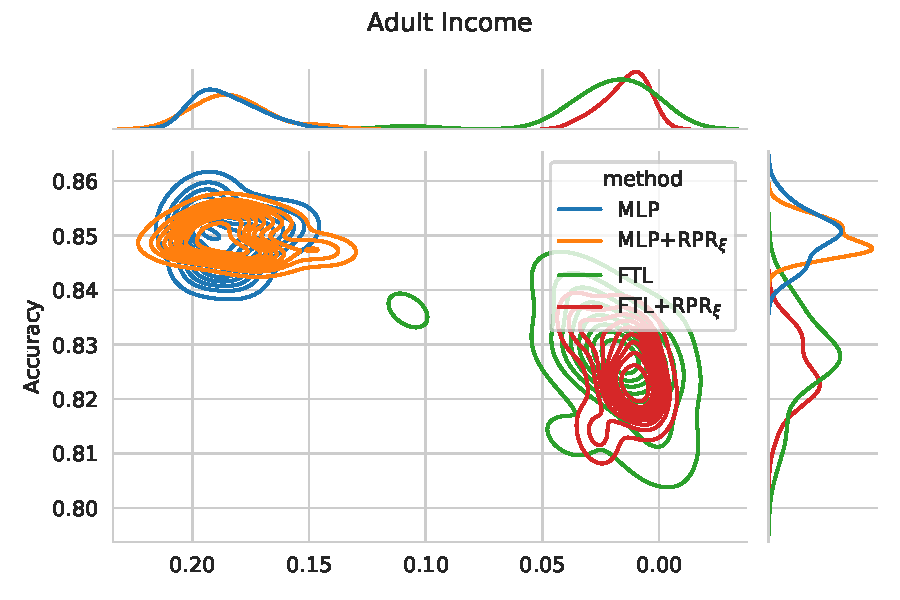
\includegraphics[width=1\linewidth]{images/pareto_acc_parity_adult_rpr.pdf}
\end{subfigure}
\begin{subfigure}{.45\linewidth}
    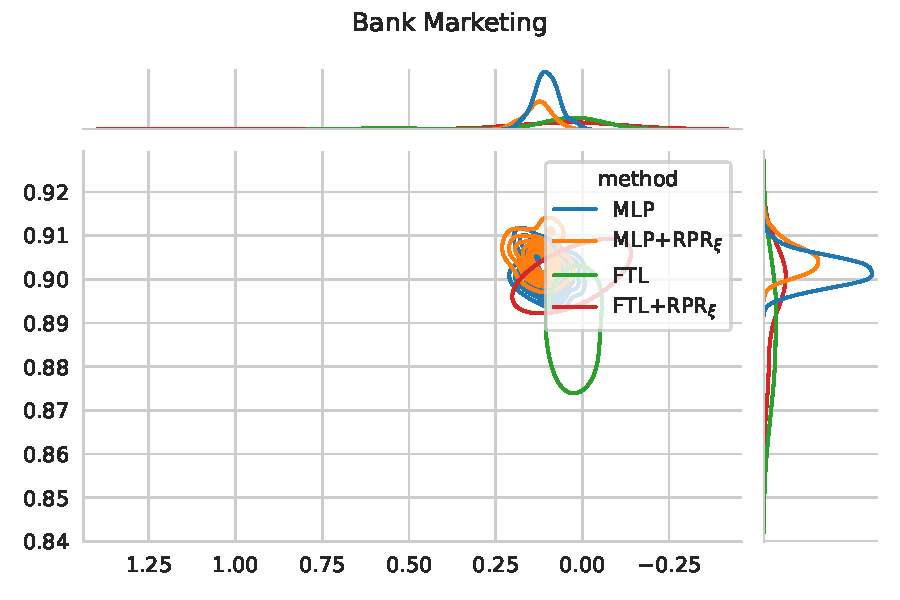
\includegraphics[width=1\linewidth]{images/pareto_acc_parity_bank_rpr.pdf}
\end{subfigure}

\begin{subfigure}{.45\linewidth}
    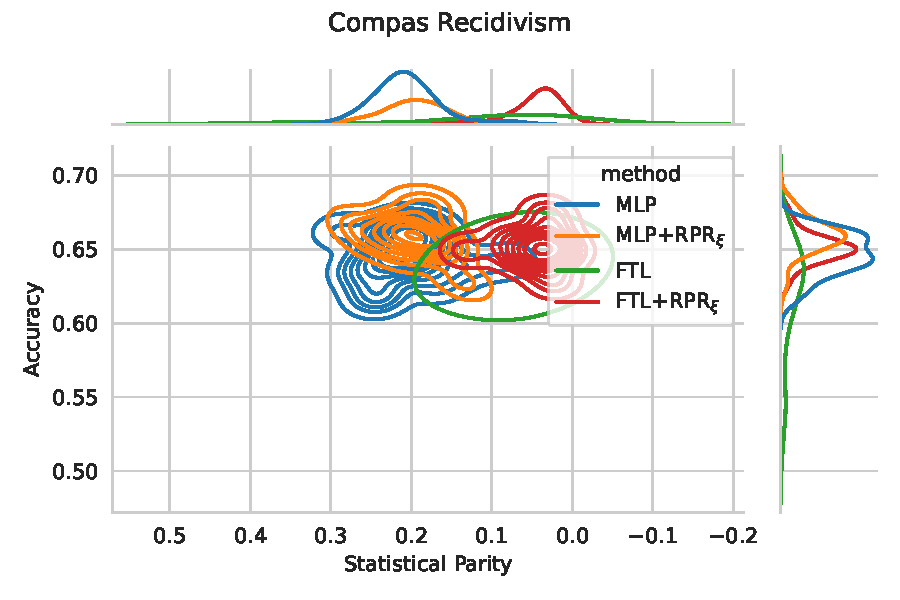
\includegraphics[width=1\linewidth]{images/pareto_acc_parity_compas_rpr.pdf}
\end{subfigure}
\begin{subfigure}{.45\linewidth}
    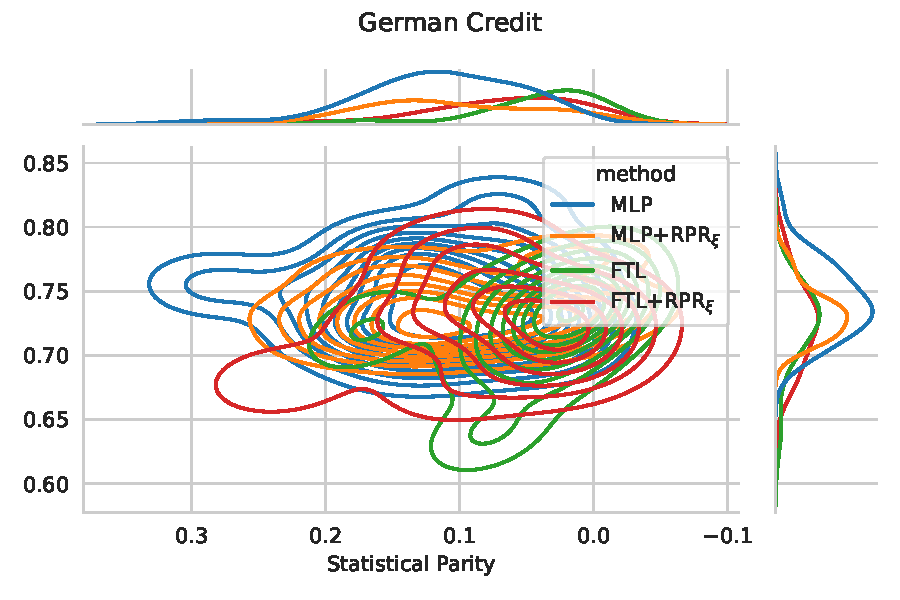
\includegraphics[width=1\linewidth]{images/pareto_acc_parity_german_rpr.pdf}
\end{subfigure}
\end{figure}

\begin{table}
    \centering
    \caption{Mean and standard deviation metric values optimizing Accuracy and Equal Opportunity in comparison with Redlining Penalty Regularizer.}\label{tab:complete_acc_opportunity_rpr}
    {\tiny \begin{tabular}{llrrr}
    \toprule
    Dataset & Method & $\uparrow\;$Fitness & $\uparrow\;$Accuracy & $\downarrow\;$Eq. Opp. \\
    \midrule
        
    \multirow{8}{*}{\shortstack[l]{Adult\\ Income}} & FTL & $0.812 \; (\pm0.03)$ & $0.845 \; (\pm0.01)$ & $0.034 \; (\pm0.02)$ \\
     & FTL+RPR$_{\xi}$ & $\textbf{0.815} \; (\pm0.02)$ & $0.847 \; (\pm0.00)$ & $\textbf{0.031} \; (\pm0.02)$ \\
     & MLP & $0.758 \; (\pm0.04)$ & $0.848 \; (\pm0.00)$ & $0.090 \; (\pm0.04)$ \\
     & MLP+L2 & $0.750 \; (\pm0.04)$ & $\textbf{0.850} \; (\pm0.00)$ & $0.100 \; (\pm0.04)$ \\
     & MLP+RPR$_{\rho_s}$ & $0.748 \; (\pm0.03)$ & $0.849 \; (\pm0.00)$ & $0.101 \; (\pm0.03)$ \\
     & MLP+RPR$_{\rho}$ & $0.750 \; (\pm0.04)$ & $0.848 \; (\pm0.00)$ & $0.098 \; (\pm0.04)$ \\
     & MLP+RPR$_{\tau}$ & $0.751 \; (\pm0.03)$ & $0.849 \; (\pm0.00)$ & $0.098 \; (\pm0.03)$ \\
     & MLP+RPR$_{\xi}$ & $0.757 \; (\pm0.05)$ & $0.849 \; (\pm0.00)$ & $0.091 \; (\pm0.05)$ \\
    \midrule
    \multirow{8}{*}{\shortstack[l]{Bank\\ Marketing}} & FTL & $0.781 \; (\pm0.17)$ & $0.883 \; (\pm0.02)$ & $0.102 \; (\pm0.17)$ \\
     & FTL+RPR$_{\xi}$ & $0.802 \; (\pm0.08)$ & $0.892 \; (\pm0.01)$ & $0.090 \; (\pm0.09)$ \\
     & MLP & $0.803 \; (\pm0.07)$ & $0.902 \; (\pm0.00)$ & $0.099 \; (\pm0.07)$ \\
     & MLP+L2 & $0.791 \; (\pm0.08)$ & $\textbf{0.903} \; (\pm0.00)$ & $0.112 \; (\pm0.07)$ \\
     & MLP+RPR$_{\rho_s}$ & $0.824 \; (\pm0.06)$ & $0.902 \; (\pm0.00)$ & $0.078 \; (\pm0.06)$ \\
     & MLP+RPR$_{\rho}$ & $0.798 \; (\pm0.07)$ & $0.901 \; (\pm0.00)$ & $0.103 \; (\pm0.07)$ \\
     & MLP+RPR$_{\tau}$ & $0.822 \; (\pm0.07)$ & $0.901 \; (\pm0.00)$ & $0.079 \; (\pm0.07)$ \\
     & MLP+RPR$_{\xi}$ & $\textbf{0.839} \; (\pm0.05)$ & $\textbf{0.903} \; (\pm0.00)$ & $\textbf{0.063} \; (\pm0.04)$ \\
    \midrule
    \multirow{8}{*}{\shortstack[l]{COMPAS\\ Recidivism}} & FTL & $\textbf{0.614} \; (\pm0.03)$ & $0.645 \; (\pm0.03)$ & $\textbf{0.031} \; (\pm0.02)$ \\
     & FTL+RPR$_{\xi}$ & $0.598 \; (\pm0.03)$ & $0.639 \; (\pm0.02)$ & $0.041 \; (\pm0.03)$ \\
     & MLP & $0.498 \; (\pm0.04)$ & $0.646 \; (\pm0.01)$ & $0.148 \; (\pm0.04)$ \\
     & MLP+L2 & $0.519 \; (\pm0.04)$ & $0.647 \; (\pm0.02)$ & $0.128 \; (\pm0.03)$ \\
     & MLP+RPR$_{\rho_s}$ & $0.520 \; (\pm0.03)$ & $0.651 \; (\pm0.01)$ & $0.131 \; (\pm0.03)$ \\
     & MLP+RPR$_{\rho}$ & $0.503 \; (\pm0.06)$ & $0.649 \; (\pm0.01)$ & $0.146 \; (\pm0.05)$ \\
     & MLP+RPR$_{\tau}$ & $0.506 \; (\pm0.04)$ & $0.647 \; (\pm0.01)$ & $0.141 \; (\pm0.04)$ \\
     & MLP+RPR$_{\xi}$ & $0.536 \; (\pm0.03)$ & $\textbf{0.663} \; (\pm0.01)$ & $0.127 \; (\pm0.03)$ \\
    \midrule
    \multirow{8}{*}{\shortstack[l]{German\\ Credit}} & FTL & $0.676 \; (\pm0.06)$ & $\textbf{0.751} \; (\pm0.02)$ & $0.075 \; (\pm0.06)$ \\
     & FTL+RPR$_{\xi}$ & $0.665 \; (\pm0.06)$ & $0.736 \; (\pm0.03)$ & $0.071 \; (\pm0.05)$ \\
     & MLP & $0.673 \; (\pm0.06)$ & $0.739 \; (\pm0.03)$ & $0.066 \; (\pm0.05)$ \\
     & MLP+L2 & $0.652 \; (\pm0.04)$ & $0.736 \; (\pm0.03)$ & $0.084 \; (\pm0.05)$ \\
     & MLP+RPR$_{\rho_s}$ & $0.667 \; (\pm0.06)$ & $0.739 \; (\pm0.03)$ & $0.072 \; (\pm0.05)$ \\
     & MLP+RPR$_{\rho}$ & $0.687 \; (\pm0.04)$ & $0.749 \; (\pm0.04)$ & $0.062 \; (\pm0.03)$ \\
     & MLP+RPR$_{\tau}$ & $\textbf{0.702} \; (\pm0.04)$ & $0.736 \; (\pm0.02)$ & $\textbf{0.034} \; (\pm0.03)$ \\
     & MLP+RPR$_{\xi}$ & $\textbf{0.702} \; (\pm0.05)$ & $0.750 \; (\pm0.02)$ & $0.048 \; (\pm0.04)$ \\
     \bottomrule
\end{tabular} }
\end{table}

\begin{figure}
\centering
\caption{Metric distribution optimizing Acc. and Equal Opportunity in comparison with Redlining Penalty Regularization across multiple resample runs. Corresponding values available at Table~\ref{tab:complete_acc_opportunity_rpr}.}
\label{fig:complete_mcc_apportunity_rpr}
\begin{subfigure}{.45\linewidth}
    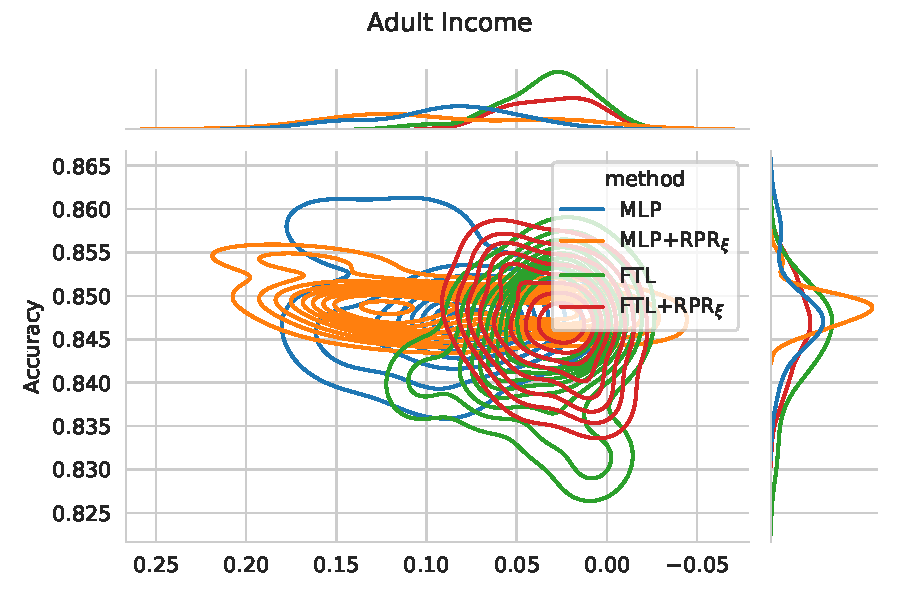
\includegraphics[width=1\linewidth]{images/pareto_acc_opportunity_adult_rpr.pdf}
\end{subfigure}
\begin{subfigure}{.45\linewidth}
    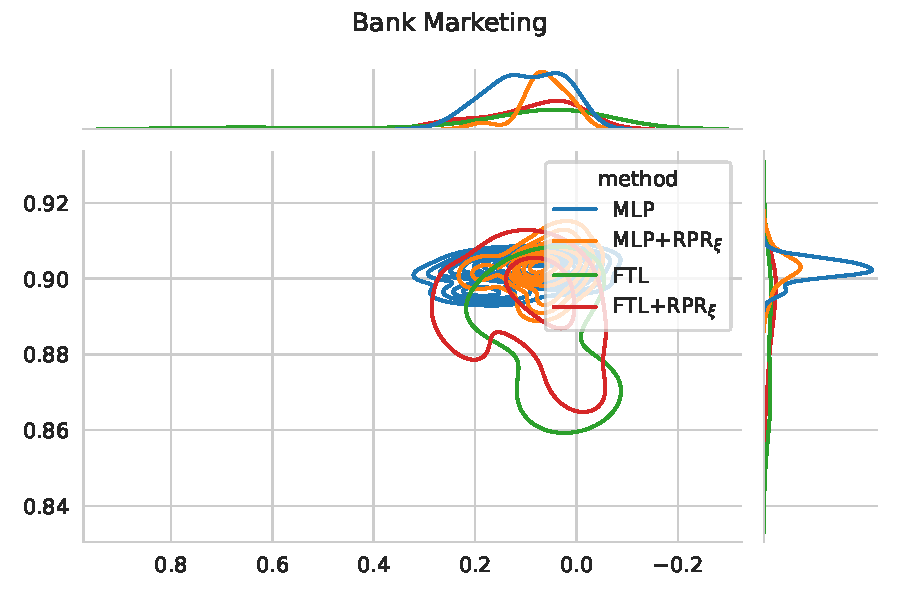
\includegraphics[width=1\linewidth]{images/pareto_acc_opportunity_bank_rpr.pdf}
\end{subfigure}

\begin{subfigure}{.45\linewidth}
    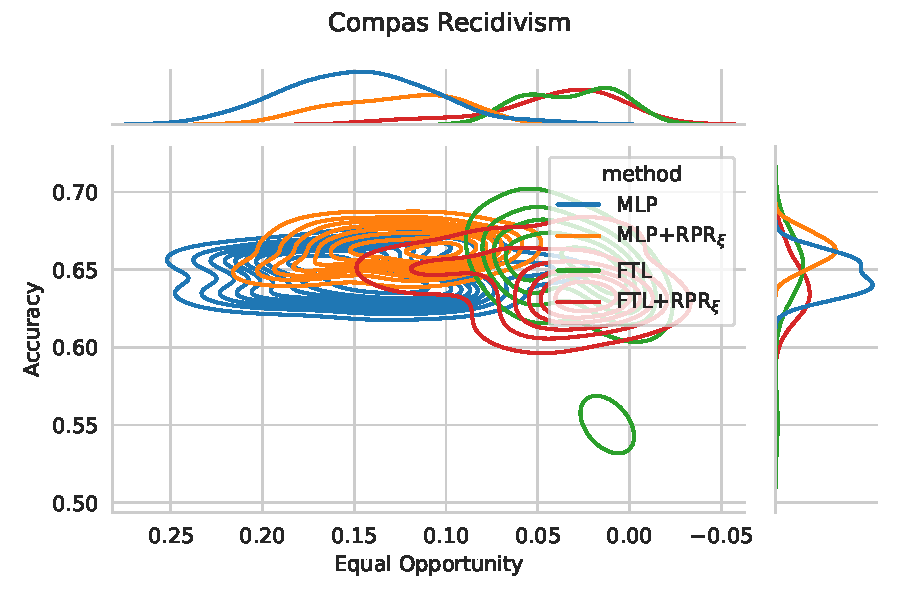
\includegraphics[width=1\linewidth]{images/pareto_acc_opportunity_compas_rpr.pdf}
\end{subfigure}
\begin{subfigure}{.45\linewidth}
    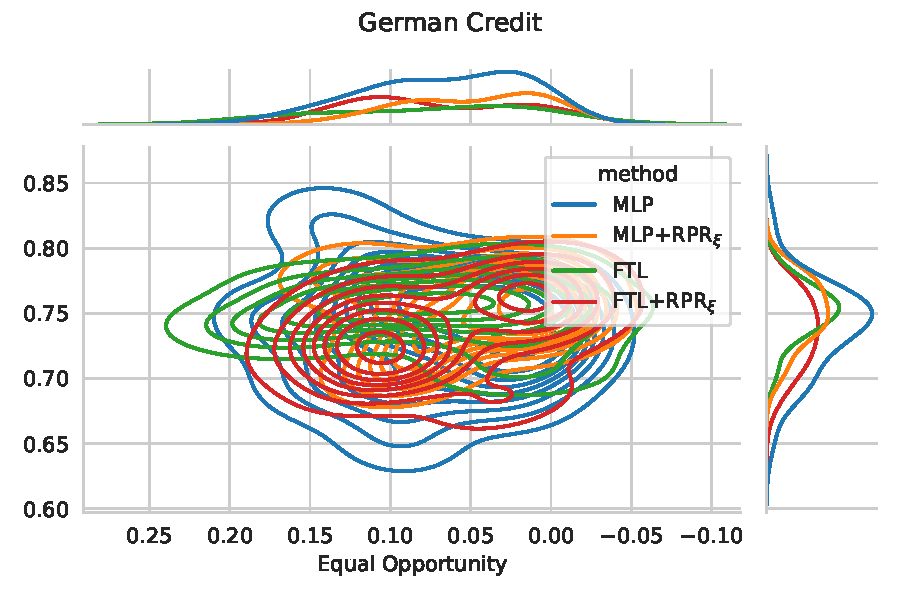
\includegraphics[width=1\linewidth]{images/pareto_acc_opportunity_german_rpr.pdf}
\end{subfigure}
\end{figure}

 \begin{table}
    \centering
    \caption{Mean and standard deviation metric values optimizing Accuracy and Equalized Odds in comparison with Redlining Penalty Regularizer.}\label{tab:complete_acc_odds_rpr}
    {\tiny \begin{tabular}{llrrr}
    \toprule
    Dataset & Method & $\uparrow\;$Fitness & $\uparrow\;$Accuracy & $\downarrow\;$Eq. Odds \\
    \midrule
        
    \multirow{8}{*}{\shortstack[l]{Adult\\ Income}} & FTL & $0.798 \; (\pm0.02)$ & $0.841 \; (\pm0.01)$ & $0.043 \; (\pm0.02)$ \\
     & FTL+RPR$_{\xi}$ & $\textbf{0.805} \; (\pm0.02)$ & $0.843 \; (\pm0.01)$ & $\textbf{0.038} \; (\pm0.02)$ \\
     & MLP & $0.760 \; (\pm0.02)$ & $\textbf{0.849} \; (\pm0.00)$ & $0.089 \; (\pm0.02)$ \\
     & MLP+L2 & $0.762 \; (\pm0.02)$ & $\textbf{0.849} \; (\pm0.00)$ & $0.086 \; (\pm0.02)$ \\
     & MLP+RPR$_{\rho_s}$ & $0.772 \; (\pm0.02)$ & $\textbf{0.849} \; (\pm0.00)$ & $0.076 \; (\pm0.02)$ \\
     & MLP+RPR$_{\rho}$ & $0.759 \; (\pm0.02)$ & $\textbf{0.849} \; (\pm0.00)$ & $0.090 \; (\pm0.02)$ \\
     & MLP+RPR$_{\tau}$ & $0.753 \; (\pm0.03)$ & $\textbf{0.849} \; (\pm0.00)$ & $0.096 \; (\pm0.02)$ \\
     & MLP+RPR$_{\xi}$ & $0.772 \; (\pm0.02)$ & $\textbf{0.849} \; (\pm0.00)$ & $0.077 \; (\pm0.02)$ \\
    \midrule
    \multirow{8}{*}{\shortstack[l]{Bank\\ Marketing}} & FTL & $\textbf{0.846} \; (\pm0.03)$ & $0.890 \; (\pm0.01)$ & $\textbf{0.044} \; (\pm0.04)$ \\
     & FTL+RPR$_{\xi}$ & $0.831 \; (\pm0.05)$ & $0.892 \; (\pm0.01)$ & $0.061 \; (\pm0.05)$ \\
     & MLP & $0.845 \; (\pm0.03)$ & $0.901 \; (\pm0.00)$ & $0.057 \; (\pm0.03)$ \\
     & MLP+L2 & $0.821 \; (\pm0.04)$ & $\textbf{0.903} \; (\pm0.00)$ & $0.082 \; (\pm0.04)$ \\
     & MLP+RPR$_{\rho_s}$ & $0.838 \; (\pm0.04)$ & $\textbf{0.903} \; (\pm0.00)$ & $0.065 \; (\pm0.04)$ \\
     & MLP+RPR$_{\rho}$ & $0.828 \; (\pm0.05)$ & $0.902 \; (\pm0.00)$ & $0.073 \; (\pm0.05)$ \\
     & MLP+RPR$_{\tau}$ & $0.822 \; (\pm0.04)$ & $0.902 \; (\pm0.00)$ & $0.079 \; (\pm0.04)$ \\
     & MLP+RPR$_{\xi}$ & $0.830 \; (\pm0.03)$ & $0.902 \; (\pm0.00)$ & $0.072 \; (\pm0.03)$ \\
    \midrule
    \multirow{8}{*}{\shortstack[l]{COMPAS\\ Recidivism}} & FTL & $0.545 \; (\pm0.10)$ & $0.631 \; (\pm0.05)$ & $0.086 \; (\pm0.08)$ \\
     & FTL+RPR$_{\xi}$ & $\textbf{0.594} \; (\pm0.04)$ & $0.647 \; (\pm0.02)$ & $\textbf{0.053} \; (\pm0.04)$ \\
     & MLP & $0.449 \; (\pm0.04)$ & $0.649 \; (\pm0.01)$ & $0.200 \; (\pm0.03)$ \\
     & MLP+L2 & $0.452 \; (\pm0.04)$ & $0.649 \; (\pm0.01)$ & $0.197 \; (\pm0.04)$ \\
     & MLP+RPR$_{\rho_s}$ & $0.464 \; (\pm0.03)$ & $0.650 \; (\pm0.01)$ & $0.186 \; (\pm0.03)$ \\
     & MLP+RPR$_{\rho}$ & $0.449 \; (\pm0.05)$ & $0.650 \; (\pm0.01)$ & $0.201 \; (\pm0.04)$ \\
     & MLP+RPR$_{\tau}$ & $0.463 \; (\pm0.05)$ & $0.650 \; (\pm0.01)$ & $0.187 \; (\pm0.05)$ \\
     & MLP+RPR$_{\xi}$ & $0.497 \; (\pm0.04)$ & $\textbf{0.667} \; (\pm0.01)$ & $0.170 \; (\pm0.03)$ \\
    \midrule
    \multirow{8}{*}{\shortstack[l]{German\\ Credit}} & FTL & $0.669 \; (\pm0.05)$ & $0.712 \; (\pm0.02)$ & $\textbf{0.043} \; (\pm0.07)$ \\
     & FTL+RPR$_{\xi}$ & $0.631 \; (\pm0.06)$ & $0.721 \; (\pm0.03)$ & $0.090 \; (\pm0.08)$ \\
     & MLP & $0.619 \; (\pm0.07)$ & $0.740 \; (\pm0.03)$ & $0.121 \; (\pm0.07)$ \\
     & MLP+L2 & $\textbf{0.675} \; (\pm0.05)$ & $\textbf{0.750} \; (\pm0.02)$ & $0.075 \; (\pm0.04)$ \\
     & MLP+RPR$_{\rho_s}$ & $0.647 \; (\pm0.06)$ & $0.742 \; (\pm0.03)$ & $0.096 \; (\pm0.05)$ \\
     & MLP+RPR$_{\rho}$ & $0.641 \; (\pm0.04)$ & $0.734 \; (\pm0.03)$ & $0.093 \; (\pm0.04)$ \\
     & MLP+RPR$_{\tau}$ & $0.647 \; (\pm0.07)$ & $0.748 \; (\pm0.03)$ & $0.101 \; (\pm0.07)$ \\
     & MLP+RPR$_{\xi}$ & $0.640 \; (\pm0.06)$ & $0.748 \; (\pm0.02)$ & $0.107 \; (\pm0.06)$ \\
     \bottomrule
\end{tabular}}
\end{table}

\begin{figure}
\centering
\caption{Metric distribution optimizing Acc. and Equalized Odds in comparison with Redlining Penalty Regularization across multiple resample runs. Corresponding values available at Table~\ref{tab:complete_acc_odds_rpr}.}
\label{fig:complete_acc_odds_rpr}
\begin{subfigure}{.45\linewidth}
    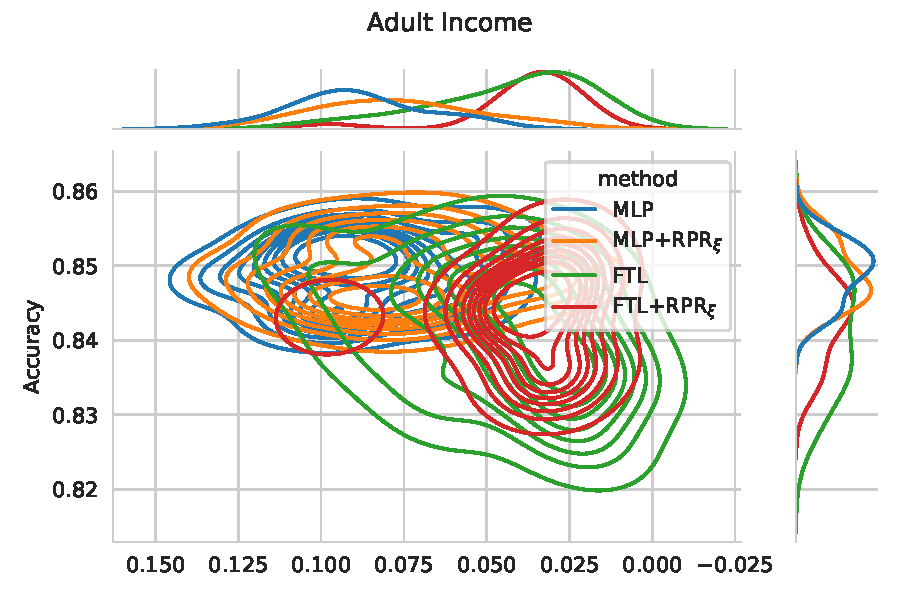
\includegraphics[width=1\linewidth]{images/pareto_acc_odds_adult_rpr.pdf}
\end{subfigure}
\begin{subfigure}{.45\linewidth}
    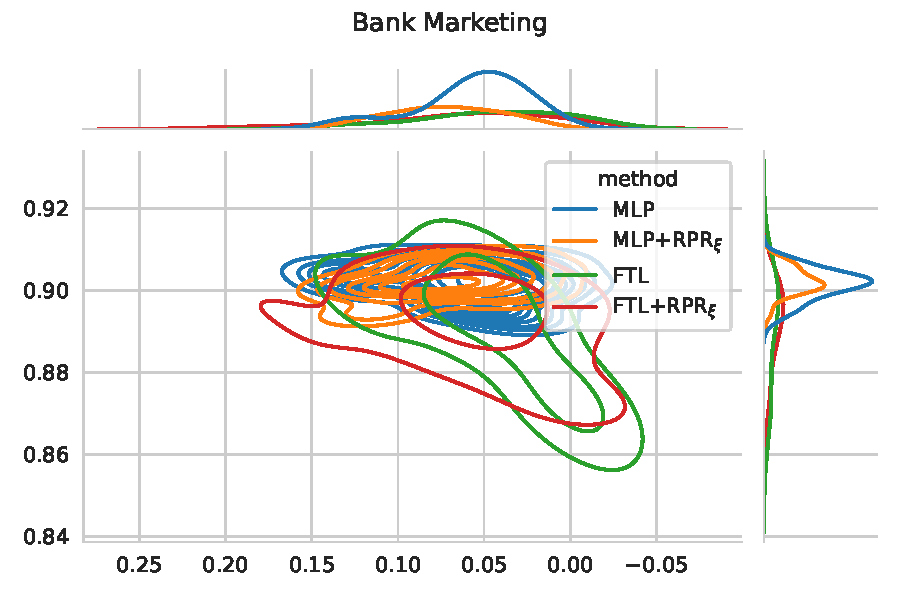
\includegraphics[width=1\linewidth]{images/pareto_acc_odds_bank_rpr.pdf}
\end{subfigure}

\begin{subfigure}{.45\linewidth}
    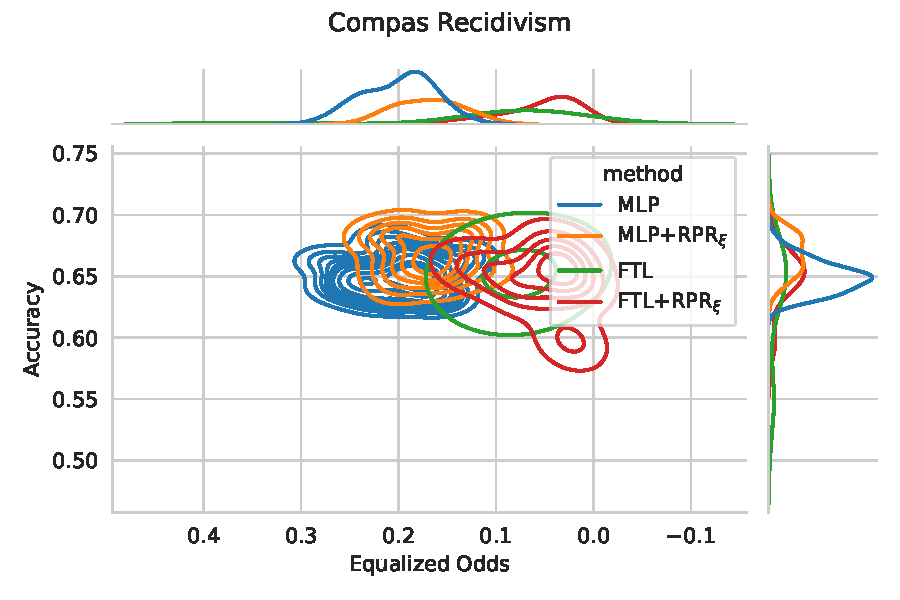
\includegraphics[width=1\linewidth]{images/pareto_acc_odds_compas_rpr.pdf}
\end{subfigure}
\begin{subfigure}{.45\linewidth}
    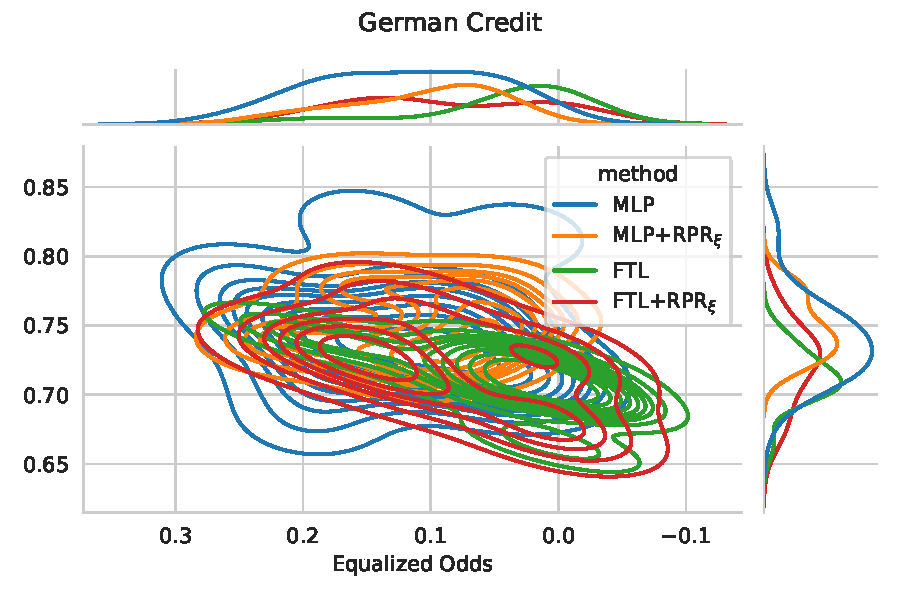
\includegraphics[width=1\linewidth]{images/pareto_acc_odds_german_rpr.pdf}
\end{subfigure}
\end{figure}

  \chapter{Conclusions}\label{chap:conclusions}


%\section{Considerations on the proposal}

In this work we introduced Fair Transition Loss, a novel approach to fair classification that estimates the influence of historical and societal biases on outcome probabilities for distinct social groups delineated by a sensitive feature. Drawing inspiration from label noise robustness, we represented these disparities on model's positive and negative outcomes probabilities to each social group using transition matrices, therefore incorporating this information onto the loss function to promote fairness. The proposed method hyperarameters were chosen by a Multi-Objective Optimization approach combining both fairness and model performance with a linear scalarization, defined in such a way that it is suitable to optimize a wide range of fairness and performance metrics.

Also, the present study proposed a novel regularization approach to fair classification named Redlining Penalty Regularization, which uses feature's correlation coefficient to the sensitive attribute to proportionately penalize model's dependency on it. Our empirical evaluation demonstrated that this approach effectively mitigate unfairness while keeping predictive performance, with benefits corresponding to redlining level on dataset. The proposed approach can be used on both standard neural networks and those trained with Fair Transition Loss to reduce bias while keeping predictive performance.

\section{Results and contributions}

Our experimental evaluation indicates that Fair Transition Loss consistently outperforms its competitors in most optimization scenarios. Even in those cases that the proposed method isn't the outright leader, it performs at least as well as evaluated alternatives, standing as the only model to keep competitive results in all scenarios. Therefore, this novel approach can significantly mitigate bias while keeping model performance, specially when optimizing balanced performance metrics like MCC. The proposed technique particularly stands out in setups where hyperparameter tuning procedures constitutes the prediction pipeline.

Furthermore, our results indicates that the Redlining Penalty Regularization approach effectively mitigates redlining effect on multiple datasets within various objective metrics when applied to both standard MLP and MLP trained with Fair Transition Loss. Also, our analysis indicates that the effectiveness of the referred approach is proportional to redlining level present on data, the higher the redlining the higher the performance-fairness trade-off improvement.

Thus, we summarize some contributions of the present study:

\begin{enumerate}[(i)]
    \item a novel loss correction approach inspired by label noise techniques to fair classification problems;
    \item a discussion of recent studies that lies between fairness and noise on machine learning;
    \item a multi-objective hyperparameter tuning approach do tackle the performance-fairness trade-off using a simple linear scalarization setup;
    \item a solid comparison of classic and state-of-art fair classification approaches using the Almost Stochastic Order as significance test;
    \item state-of-art results on various benchmarked datasets to fair classification using the proposed loss correction approach;
    \item a novel regularization approach that proportionately penalizes model's dependency on sensitive feature proxies according their correlations;
    \item improved results using the proposed regularization approach on standard MLPs to fair classification.
    \item improved state-of-art results using both the loss correction and regularization approaches to fair classification.
\end{enumerate}

\section{Research directions}

Here we outline some research direction insights, derived from proposed method's drawbacks and issues uncharted by this study:

\begin{enumerate}[(i)]
    \item explore approaches to estimating or initializing transition matrices to reduce computational costs required by hyperparameter optimization techniques;
    \item evaluate Fair Transition Loss within different neural network architectures, such as Deep Neural Networks;
    \item evaluate Fair Transition Loss on different data domains, such as image, audio and natural language;
    \item evaluate Fair Transition Loss optimization under non-linear scalarization setups, such as the Chebyshev scalarization scheme proposed by~\cite{Wei2022};
    \item evaluate Fair Transition Loss within different multi-objective optimization schemes, such as the Fair Hyperparameter Tuning techniques proposed by~\cite{Cruz2021};
    \item investigate whether Fair Transition Loss can effectively address multi-class fair classification problems and handle multiple sensitive attributes, as theoretically possible;
    \item evaluate Redlining Penalty Regularization within different neural network architectures, such as Deep Neural Networks;
    \item evaluate Redlining Penalty Regularization on different data domains, such as image, audio and natural language;
    \item evaluate Redlining Penalty Regularization combined with multiple pre-processing, in-processing and post-processing fair classification approaches.
    
\end{enumerate}



 
  %\chapter{Proposta}
  %\section{Ruído e Injustiça}
  %\section{Função de custo de transição para aprendizado justo}
  %\section{Correlação e preditores indiretos}
  %\section{Regularização}
  %\section{Ajuste de hiperparâmetros e matrizes de transição}

  %\chapter{Resultados e discussão}
  %\section{Significância para redes profundas}
  %\section{Estudo comparativo da função de custo de transição}
  %\section{Estudo comparativo com regularização}

  %\chapter{Conclusões}
  


  %\chapter{Conclusões}

  \backmatter
  \bibliographystyle{coppe-unsrt}
  \bibliography{thesis}

  %\appendix
  \include{appendix}
\end{document}
%% 
%%
%% End of file `example.tex'.
